% power_diode_fundamentals.tex
% Fundamentals of semiconductor devices: the power diode.
% English version of power_diode_fundamentals_it.tex (same structure, same labels, same equations).
% One document that collects and harmonises three notes of this folder (research/power_semiconductor_devices/diode):
%   power_diode/power_diode.tex                        PIN structure, bands, conduction, reverse recovery, technologies (IT)
%   charge_control_model/charge_control.tex            ambipolar equation and charge-control model (IT)
%   lauritzen_ma_datasheet_conversion/....tex          Lauritzen-Ma model and conversion of datasheet data (EN, IT)
% The three notes stay where they are; Appendix C lists the correspondence of the symbols and what was corrected.
% pwr-control template (AAA_template_latex_settings). Numbers and figures:
%   power_diode_fundamentals_calc.py  ->  power_diode_fundamentals_values.tex (macros \pd...), figures/fig_*.pdf
%   ../lauritzen_ma_datasheet_conversion/lm_conversion_calc.py  ->  lm_conversion_values.tex (macros \lm...),
%   figures/fig_*.pdf of that folder: this document reads them from there, without copying them
% Compile, from this folder: pdflatex power_diode_fundamentals.tex  (three times, for contents and references)
% Rev. 00 - November 2026 - first issue
\documentclass[10pt,a4paper]{scrartcl}
\input{../../../../AAA_template_latex_settings/settings}
% the document sits four levels below the repository root: logo path of settings.tex corrected here
\rhead{\includegraphics[height=0.75cm]{../../../../AAA_template_latex_settings/pwr-control_logo_doc.png}}
\rfoot{\small Rev.~00}
\geometry{left=2.0cm, right=2.0cm}\setlength{\headwidth}{\textwidth}
\usepackage[european resistors, american inductors]{circuitikz}
\usetikzlibrary{patterns}
\usepackage[T1]{fontenc}\usepackage{lmodern}   % T1 and Latin Modern: in the PDF accented letters and underscores are real characters (text search and copy) and no font is a bitmap
\sisetup{per-mode=symbol,range-phrase={\text{--}},range-units=single}
\setlist{nosep}
\setlength{\parindent}{0pt}
\setlength{\parskip}{3pt}
\allowdisplaybreaks
\widowpenalty=10000 \clubpenalty=10000 \makeatletter\@clubpenalty=\clubpenalty\makeatother \displaywidowpenalty=10000   % no single line alone at the top or at the bottom of a page, nor before a displayed formula
\captionsetup{font=small,labelfont=bf}
\RedeclareSectionCommand[tocnumwidth=2.2em]{section}   % contents: room for two-digit section numbers
\RedeclareSectionCommand[tocindent=2.2em,tocnumwidth=3.0em]{subsection}
\renewcommand{\topfraction}{0.9}
\renewcommand{\bottomfraction}{0.9}
\renewcommand{\textfraction}{0.05}
\renewcommand{\floatpagefraction}{0.8}

% --- numbers (generated by the two scripts) ---
% generated by power_diode_fundamentals_calc.py: do not edit by hand
\newcommand{\pdVt}{25.85}
\newcommand{\pdMun}{1400}
\newcommand{\pdMup}{450}
\newcommand{\pdMusum}{1850}
\newcommand{\pdDn}{36}
\newcommand{\pdDp}{12}
\newcommand{\pdDa}{18}
\newcommand{\pdDaOne}{17.6}
\newcommand{\pdBratio}{3.1}
\newcommand{\pdBmob}{0.51}
\newcommand{\pdOneMinusBsq}{0.74}
\newcommand{\pdSigmaRatio}{1.32}
\newcommand{\pdEpsR}{11.7}
\newcommand{\pdEpsFcm}{1.04}
\newcommand{\pdLaOne}{42}
\newcommand{\pdLaTen}{133}
\newcommand{\pdVmAsymCoef}{1.35}
\newcommand{\pdVmHandCoef}{1.18}
\newcommand{\pdThreePiEight}{1.18}
\newcommand{\pdDaHotA}{12}
\newcommand{\pdDaHotB}{11}
\newcommand{\pdNiDoubleLo}{8}
\newcommand{\pdNiDoubleHi}{15}
\newcommand{\pdNiRatio}{540}
\newcommand{\pdEgZero}{1.2}
\newcommand{\pdTcVjLo}{0.60}
\newcommand{\pdTcLo}{2.3}
\newcommand{\pdTcVjHi}{0.82}
\newcommand{\pdTcHi}{1.5}
\newcommand{\pdTauAugerLo}{263}
\newcommand{\pdTauAugerHi}{2.6}
\newcommand{\pdBlkNdA}{2\times10^{13}}
\newcommand{\pdBlkEcA}{1.84}
\newcommand{\pdBlkVA}{5500}
\newcommand{\pdBlkWA}{596}
\newcommand{\pdBlkRA}{13.29}
\newcommand{\pdBlkDropA}{1329}
\newcommand{\pdBlkNdB}{5\times10^{13}}
\newcommand{\pdBlkEcB}{2.07}
\newcommand{\pdBlkVB}{2760}
\newcommand{\pdBlkWB}{267}
\newcommand{\pdBlkRB}{2.38}
\newcommand{\pdBlkDropB}{238}
\newcommand{\pdBlkNdC}{1\times10^{14}}
\newcommand{\pdBlkEcC}{2.25}
\newcommand{\pdBlkVC}{1640}
\newcommand{\pdBlkWC}{146}
\newcommand{\pdBlkRC}{0.65}
\newcommand{\pdBlkDropC}{65}
\newcommand{\pdBlkNdD}{2\times10^{14}}
\newcommand{\pdBlkEcD}{2.46}
\newcommand{\pdBlkVD}{980}
\newcommand{\pdBlkWD}{80}
\newcommand{\pdBlkRD}{0.18}
\newcommand{\pdBlkDropD}{18}
\newcommand{\pdBlkCoefV}{5.2\times10^{13}}
\newcommand{\pdBlkCoefW}{2.6\times10^{10}}
\newcommand{\pdTgtV}{2}
\newcommand{\pdTgtNd}{7.7\times10^{13}}
\newcommand{\pdTgtW}{183}
\newcommand{\pdTgtR}{1.1}
\newcommand{\pdTgtDrop}{110}
\newcommand{\pdPtNd}{3\times10^{13}}
\newcommand{\pdPtW}{120}
\newcommand{\pdPtSavePct}{34}
\newcommand{\pdPtEc}{1.94}
\newcommand{\pdExVbr}{1480}
\newcommand{\pdDynPLo}{6.2\times10^{13}}
\newcommand{\pdDynPctLo}{62}
\newcommand{\pdDynJLo}{100}
\newcommand{\pdDynVbrLo}{1140}
\newcommand{\pdDynPHi}{1.9\times10^{14}}
\newcommand{\pdDynPctHi}{187}
\newcommand{\pdDynJHi}{300}
\newcommand{\pdDynVbrHi}{750}
\newcommand{\pdVbi}{0.77}
\newcommand{\pdVbiTwo}{0.30}
\newcommand{\pdScV}{600}
\newcommand{\pdScWZero}{3.2}
\newcommand{\pdScW}{88}
\newcommand{\pdScCjZero}{3.3}
\newcommand{\pdScCj}{120}
\newcommand{\pdScQc}{0.14}
\newcommand{\pdExVrt}{770}
\newcommand{\pdScQcPct}{0.14}
\newcommand{\pdJgenUa}{14}
\newcommand{\pdExW}{100}
\newcommand{\pdExNd}{1\times10^{14}}
\newcommand{\pdExJ}{100}
\newcommand{\pdExRuni}{0.45}
\newcommand{\pdExDropUni}{45}
\newcommand{\pdExNa}{1\times10^{19}}
\newcommand{\pdHem}{2\times10^{-14}}
\newcommand{\pdExRho}{45}
\newcommand{\pdLpOne}{34}
\newcommand{\pdJsShockley}{5.5\times10^{-10}}
\newcommand{\pdHiOnsetV}{0.48}
\newcommand{\pdHiOnsetJ}{50}
\newcommand{\pdExSlowTau}{10}
\newcommand{\pdExSlowLa}{133}
\newcommand{\pdExSlowBeta}{0.38}
\newcommand{\pdExSlowPbar}{6.2\times10^{17}}
\newcommand{\pdExSlowPl}{7.0\times10^{17}}
\newcommand{\pdExSlowPr}{6.1\times10^{17}}
\newcommand{\pdExSlowPmin}{6.0\times10^{17}}
\newcommand{\pdExSlowQs}{1000}
\newcommand{\pdExSlowSigRatio}{8250}
\newcommand{\pdExSlowVmFlat}{5}
\newcommand{\pdExSlowVm}{7}
\newcommand{\pdExSlowVmOhm}{5}
\newcommand{\pdExSlowVmDem}{2}
\newcommand{\pdExSlowVmThin}{7}
\newcommand{\pdExSlowVjOne}{0.70}
\newcommand{\pdExSlowVjTwo}{0.23}
\newcommand{\pdExSlowVf}{0.94}
\newcommand{\pdExSlowTmStat}{0.05}
\newcommand{\pdExSlowEmQs}{171}
\newcommand{\pdExSlowEmTauEff}{1.71}
\newcommand{\pdExSlowEmTauPct}{17}
\newcommand{\pdExSlowEmPct}{83}
\newcommand{\pdExSlowEmVf}{0.88}
\newcommand{\pdExSlowEmVm}{37}
\newcommand{\pdExSlowEmPl}{1.3\times10^{17}}
\newcommand{\pdExSlowEmPr}{9.2\times10^{16}}
\newcommand{\pdExSlowEmPbar}{1.1\times10^{17}}
\newcommand{\pdExSlowEmSlopeVj}{1.07}
\newcommand{\pdExSlowEmSlopeVf}{1.67}
\newcommand{\pdExSlowQflOne}{0.93}
\newcommand{\pdExSlowTauAuger}{7}
\newcommand{\pdExMidTau}{1}
\newcommand{\pdExMidLa}{42}
\newcommand{\pdExMidBeta}{1.19}
\newcommand{\pdExMidPbar}{6.2\times10^{16}}
\newcommand{\pdExMidPl}{1.2\times10^{17}}
\newcommand{\pdExMidPr}{5.8\times10^{16}}
\newcommand{\pdExMidPmin}{4.5\times10^{16}}
\newcommand{\pdExMidQs}{100}
\newcommand{\pdExMidSigRatio}{820}
\newcommand{\pdExMidVmFlat}{54}
\newcommand{\pdExMidVm}{69}
\newcommand{\pdExMidVmOhm}{59}
\newcommand{\pdExMidVmDem}{10}
\newcommand{\pdExMidVmThin}{73}
\newcommand{\pdExMidVjOne}{0.66}
\newcommand{\pdExMidVjTwo}{0.16}
\newcommand{\pdExMidVf}{0.89}
\newcommand{\pdExMidTmStat}{0.43}
\newcommand{\pdExMidEmQs}{71}
\newcommand{\pdExMidEmTauEff}{0.71}
\newcommand{\pdExMidEmTauPct}{71}
\newcommand{\pdExMidEmPct}{29}
\newcommand{\pdExMidEmVf}{0.90}
\newcommand{\pdExMidEmVm}{91}
\newcommand{\pdExMidEmPl}{8.5\times10^{16}}
\newcommand{\pdExMidEmPr}{4.3\times10^{16}}
\newcommand{\pdExMidEmPbar}{4.4\times10^{16}}
\newcommand{\pdExMidEmSlopeVj}{1.57}
\newcommand{\pdExMidEmSlopeVf}{2.24}
\newcommand{\pdExMidQflOne}{0.84}
\newcommand{\pdExMidTauAuger}{676}
\newcommand{\pdExFastTau}{0.3}
\newcommand{\pdExFastLa}{23}
\newcommand{\pdExFastBeta}{2.18}
\newcommand{\pdExFastPbar}{1.9\times10^{16}}
\newcommand{\pdExFastPl}{6.2\times10^{16}}
\newcommand{\pdExFastPr}{2.1\times10^{16}}
\newcommand{\pdExFastPmin}{8.1\times10^{15}}
\newcommand{\pdExFastQs}{30}
\newcommand{\pdExFastSigRatio}{250}
\newcommand{\pdExFastVmFlat}{180}
\newcommand{\pdExFastVm}{265}
\newcommand{\pdExFastVmOhm}{251}
\newcommand{\pdExFastVmDem}{14}
\newcommand{\pdExFastVmThin}{245}
\newcommand{\pdExFastVjOne}{0.64}
\newcommand{\pdExFastVjTwo}{0.14}
\newcommand{\pdExFastVf}{1.05}
\newcommand{\pdExFastTmStat}{1.23}
\newcommand{\pdExFastEmQs}{27}
\newcommand{\pdExFastEmTauEff}{0.27}
\newcommand{\pdExFastEmTauPct}{89}
\newcommand{\pdExFastEmPct}{11}
\newcommand{\pdExFastEmVf}{1.07}
\newcommand{\pdExFastEmVm}{290}
\newcommand{\pdExFastEmPl}{5.4\times10^{16}}
\newcommand{\pdExFastEmPr}{2.0\times10^{16}}
\newcommand{\pdExFastEmPbar}{1.7\times10^{16}}
\newcommand{\pdExFastEmSlopeVj}{1.83}
\newcommand{\pdExFastEmSlopeVf}{2.71}
\newcommand{\pdExFastQflOne}{0.81}
\newcommand{\pdExFastTauAuger}{7506}
\newcommand{\pdVmHalfVt}{0.48}
\newcommand{\pdVmHalfMv}{12}
\newcommand{\pdVmThinErrHalfPct}{3}
\newcommand{\pdVmAsymErrHalfPct}{360}
\newcommand{\pdVmHandErrHalfPct}{302}
\newcommand{\pdVmThinSgnHalf}{+3}
\newcommand{\pdVmAsymSgnHalf}{+360}
\newcommand{\pdVmHandSgnHalf}{+302}
\newcommand{\pdVmFlatLowHalfPct}{24}
\newcommand{\pdVmOneVt}{1.87}
\newcommand{\pdVmOneMv}{48}
\newcommand{\pdVmThinErrOnePct}{7}
\newcommand{\pdVmAsymErrOnePct}{96}
\newcommand{\pdVmHandErrOnePct}{72}
\newcommand{\pdVmThinSgnOne}{+7}
\newcommand{\pdVmAsymSgnOne}{+96}
\newcommand{\pdVmHandSgnOne}{+72}
\newcommand{\pdVmFlatLowOnePct}{21}
\newcommand{\pdVmTwoVt}{8.30}
\newcommand{\pdVmTwoMv}{215}
\newcommand{\pdVmThinErrTwoPct}{4}
\newcommand{\pdVmAsymErrTwoPct}{20}
\newcommand{\pdVmHandErrTwoPct}{5}
\newcommand{\pdVmThinSgnTwo}{-4}
\newcommand{\pdVmAsymSgnTwo}{+20}
\newcommand{\pdVmHandSgnTwo}{+5}
\newcommand{\pdVmFlatLowTwoPct}{29}
\newcommand{\pdVmThreeVt}{25.5}
\newcommand{\pdVmThreeMv}{661}
\newcommand{\pdVmThinErrThreePct}{30}
\newcommand{\pdVmAsymErrThreePct}{6}
\newcommand{\pdVmHandErrThreePct}{7}
\newcommand{\pdVmThinSgnThree}{-30}
\newcommand{\pdVmAsymSgnThree}{+6}
\newcommand{\pdVmHandSgnThree}{-7}
\newcommand{\pdVmFlatLowThreePct}{48}
\newcommand{\pdVmFourVt}{72.1}
\newcommand{\pdVmFourMv}{1865}
\newcommand{\pdVmThinErrFourPct}{56}
\newcommand{\pdVmAsymErrFourPct}{2}
\newcommand{\pdVmHandErrFourPct}{11}
\newcommand{\pdVmThinSgnFour}{-56}
\newcommand{\pdVmAsymSgnFour}{+2}
\newcommand{\pdVmHandSgnFour}{-11}
\newcommand{\pdVmFlatLowFourPct}{67}
\newcommand{\pdVmFlatLowPct}{26}
\newcommand{\pdDemberLimit}{0.58}
\newcommand{\pdVfMinBeta}{0.95}
\newcommand{\pdVfMinTau}{1.6}
\newcommand{\pdVfMin}{0.89}
\newcommand{\pdVfFlatLo}{0.7}
\newcommand{\pdVfFlatHi}{1.3}
\newcommand{\pdExMidSigma}{18}
\newcommand{\pdRelaxFs}{60}
\newcommand{\pdDebyeNm}{12}
\newcommand{\pdRelaxPs}{50}
\newcommand{\pdExTmPar}{470}
\newcommand{\pdExTmMode}{580}
\newcommand{\pdEmJLo}{10}
\newcommand{\pdEmJLoTauEff}{0.95}
\newcommand{\pdEmJLoPct}{5}
\newcommand{\pdEmJMid}{100}
\newcommand{\pdEmJMidTauEff}{0.71}
\newcommand{\pdEmJMidPct}{29}
\newcommand{\pdEmJHi}{300}
\newcommand{\pdEmJHiTauEff}{0.53}
\newcommand{\pdEmJHiPct}{47}
\newcommand{\pdTsOne}{0.69}
\newcommand{\pdTsFour}{1.61}
\newcommand{\pdRampFracFast}{91}
\newcommand{\pdRampLamFast}{0.2}
\newcommand{\pdRampFracMid}{63}
\newcommand{\pdRampLamMid}{1.0}
\newcommand{\pdRampFracSlow}{20}
\newcommand{\pdRampLamSlow}{5.0}
\newcommand{\pdRampYFast}{0.51}
\newcommand{\pdRampQrrFast}{64}
\newcommand{\pdRampIrrIfFast}{2.53}
\newcommand{\pdRampYMid}{0.84}
\newcommand{\pdRampQrrMid}{35}
\newcommand{\pdRampIrrIfMid}{0.84}
\newcommand{\pdRampYSlow}{1.00}
\newcommand{\pdRampQrrSlow}{10}
\newcommand{\pdRampIrrIfSlow}{0.20}
\newcommand{\pdTmModeRatioPct}{22}
\newcommand{\pdTmAsymFactor}{2.5}
\newcommand{\pdDistTaQuarter}{0.95}
\newcommand{\pdDistTmQuarter}{0.051}
\newcommand{\pdDistTmGeomQuarter}{2.47}
\newcommand{\pdDistSQuarter}{0.10}
\newcommand{\pdDistTauFitQuarter}{1.00}
\newcommand{\pdDistTmFitQuarter}{0.051}
\newcommand{\pdDistWidthQuarter}{1.56}
\newcommand{\pdTmPeakPosQuarter}{0.50}
\newcommand{\pdTmBlockSymQuarter}{0.99}
\newcommand{\pdTmBlockAsymQuarter}{2.5}
\newcommand{\pdDistTaHalf}{0.84}
\newcommand{\pdDistTmHalf}{0.189}
\newcommand{\pdDistTmGeomHalf}{2.26}
\newcommand{\pdDistSHalf}{0.36}
\newcommand{\pdDistTauFitHalf}{0.99}
\newcommand{\pdDistTmFitHalf}{0.176}
\newcommand{\pdDistWidthHalf}{1.45}
\newcommand{\pdTmPeakPosHalf}{0.45}
\newcommand{\pdTmBlockSymHalf}{0.97}
\newcommand{\pdTmBlockAsymHalf}{2.3}
\newcommand{\pdDistTaOne}{0.65}
\newcommand{\pdDistTmOne}{0.540}
\newcommand{\pdDistTmGeomOne}{1.62}
\newcommand{\pdDistSOne}{0.86}
\newcommand{\pdDistTauFitOne}{0.93}
\newcommand{\pdDistTmFitOne}{0.398}
\newcommand{\pdDistWidthOne}{1.09}
\newcommand{\pdTmPeakPosOne}{0.23}
\newcommand{\pdTmBlockSymOne}{0.87}
\newcommand{\pdTmBlockAsymOne}{1.6}
\newcommand{\pdDistTaOneHalf}{0.56}
\newcommand{\pdDistTmOneHalf}{0.782}
\newcommand{\pdDistTmGeomOneHalf}{1.04}
\newcommand{\pdDistSOneHalf}{1.04}
\newcommand{\pdDistTauFitOneHalf}{0.85}
\newcommand{\pdDistTmFitOneHalf}{0.442}
\newcommand{\pdDistWidthOneHalf}{0.77}
\newcommand{\pdTmPeakPosOneHalf}{-0.13}
\newcommand{\pdDistTaTwo}{0.53}
\newcommand{\pdDistTmTwo}{0.901}
\newcommand{\pdDistTmGeomTwo}{0.68}
\newcommand{\pdDistSTwo}{1.06}
\newcommand{\pdDistTauFitTwo}{0.80}
\newcommand{\pdDistTmFitTwo}{0.426}
\newcommand{\pdDistWidthTwo}{0.57}
\newcommand{\pdTmPeakPosTwo}{-0.42}
\newcommand{\pdDistTaThree}{0.50}
\newcommand{\pdDistTmThree}{0.981}
\newcommand{\pdDistTmGeomThree}{0.33}
\newcommand{\pdDistSThree}{1.03}
\newcommand{\pdDistTauFitThree}{0.76}
\newcommand{\pdDistTmFitThree}{0.393}
\newcommand{\pdDistWidthThree}{0.36}
\newcommand{\pdTmPeakPosThree}{-0.66}
\newcommand{\pdDistSmax}{1.06}
\newcommand{\pdDistSmaxBeta}{1.9}
\newcommand{\pdDistSoneBeta}{1.3}
\newcommand{\pdDistSmaxSym}{1.11}
\newcommand{\pdDistSmaxBetaSym}{2.4}
\newcommand{\pdDistSoneBetaSym}{1.7}
\newcommand{\pdTmPeakZeroBeta}{1.3}
\newcommand{\pdTmTailCoef}{1.1}
\newcommand{\pdTmTailFactor}{3.3}
\newcommand{\pdTmTailCoefSym}{0.41}
\newcommand{\pdTmTailAngle}{1.90}
\newcommand{\pdAWblock}{336}
\newcommand{\pdAWtail}{294}
\newcommand{\pdAWlawPct}{2}
\newcommand{\pdBWblock}{33}
\newcommand{\pdBWtail}{29}
\newcommand{\pdBWlawPct}{2}
\newcommand{\pdADistBeta}{1.57}
\newcommand{\pdADistTau}{45}
\newcommand{\pdADistW}{730}
\newcommand{\pdADistWmm}{0.7}
\newcommand{\pdADistBetaHi}{2.48}
\newcommand{\pdADistTauHi}{49}
\newcommand{\pdADistWHi}{1210}
\newcommand{\pdADistWmmHi}{1.2}
\newcommand{\pdADistLoBeta}{1.3}
\newcommand{\pdADistLoW}{590}
\newcommand{\pdADistLoWmm}{0.6}
\newcommand{\pdADistLoPct}{2.4}
\newcommand{\pdADistMaxPct}{0.7}
\newcommand{\pdADistInfPct}{2.3}
\newcommand{\pdADistTol}{2.4}
\newcommand{\pdADistTauLo}{43}
\newcommand{\pdADistTauInf}{50}
\newcommand{\pdBDistSmax}{1.33}
\newcommand{\pdBDistSmaxBeta}{1.6}
\newcommand{\pdBDistSmaxSym}{1.40}
\newcommand{\pdBDistSmaxBetaSym}{2.0}
\newcommand{\pdAVpkCjPeriod}{1.0}
\newcommand{\pdAVpkCj}{850}
\newcommand{\pdAVpkCjSim}{840}
\newcommand{\pdAVpkCjRatio}{2.9}
\newcommand{\pdBVpkCjPeriod}{28}
\newcommand{\pdBVpkCj}{3060}
\newcommand{\pdBVpkCjSim}{3010}
\newcommand{\pdBVpkCjRatio}{3.0}
\newcommand{\pdALongSlopeFive}{6}
\newcommand{\pdALongSlopeThree}{11}
\newcommand{\pdATenXi}{3.3}
\newcommand{\pdATenIrrPct}{4}
\newcommand{\pdATenQrrPct}{6}
\newcommand{\pdSwErecIdeal}{7.2}
\newcommand{\pdSwErecDiode}{5.3}
\newcommand{\pdSwK}{0.73}
\newcommand{\pdSwEonExtra}{6.7}
\newcommand{\pdSwEonLoad}{4.8}
\newcommand{\pdSwEonQa}{1.9}
\newcommand{\pdSwRatio}{1.3}
\newcommand{\pdSwLs}{50}
\newcommand{\pdSwOvSoft}{36}
\newcommand{\pdSwOvSnap}{200}
\newcommand{\pdSwSnapS}{0.5}
\newcommand{\pdSwOvIdeal}{440}
\newcommand{\pdExVmTau}{73}
\newcommand{\pdOcvdSlope}{52}
\newcommand{\pdSiUniR}{0.30}
\newcommand{\pdSiUniDrop}{30}
\newcommand{\pdSiUniW}{101}

% generated by lm_conversion_calc.py: do not edit by hand
\newcommand{\lmKLine}{1.879}
\newcommand{\lmKTen}{2.303}
\newcommand{\lmKQuarter}{1.386}
\newcommand{\lmKLineHalf}{0.94}
\newcommand{\lmKLineLossPct}{6}
\newcommand{\lmKTenGainPct}{15}
\newcommand{\lmKSpread}{0.92}
\newcommand{\lmTEndTaus}{3.9}
\newcommand{\lmPEndPct}{2}
\newcommand{\lmTailFrac}{0.98}
\newcommand{\lmSofStretchThree}{1.74}
\newcommand{\lmFDefTwo}{13.5}
\newcommand{\lmQDefLoTwo}{17.4}
\newcommand{\lmQDefHiTwo}{23.1}
\newcommand{\lmFDefThree}{5.0}
\newcommand{\lmQDefLoThree}{6.6}
\newcommand{\lmQDefHiThree}{8.8}
\newcommand{\lmFDefFour}{1.8}
\newcommand{\lmQDefLoFour}{2.4}
\newcommand{\lmQDefHiFour}{3.3}
\newcommand{\lmFDefFive}{0.7}
\newcommand{\lmQDefLoFive}{0.9}
\newcommand{\lmQDefHiFive}{1.2}
\newcommand{\lmXLong}{3}
\newcommand{\lmQfracRhoLo}{48}
\newcommand{\lmSofRhoLo}{0.50}
\newcommand{\lmQfracRhoMid}{44}
\newcommand{\lmSofRhoMid}{1.08}
\newcommand{\lmQfracRhoHi}{38}
\newcommand{\lmSofRhoHi}{2.00}
\newcommand{\lmTenthErrTwo}{0.6}
\newcommand{\lmTenthErrFour}{3.1}
\newcommand{\lmRatioLoOne}{0.08}
\newcommand{\lmRatioHiOne}{0.21}
\newcommand{\lmRatioOneHalf}{0.21}
\newcommand{\lmRatioOneOne}{0.17}
\newcommand{\lmRatioOneTwo}{0.12}
\newcommand{\lmRatioOneFour}{0.08}
\newcommand{\lmRatioLoFive}{0.12}
\newcommand{\lmRatioHiFive}{0.36}
\newcommand{\lmRatioFiveHalf}{0.36}
\newcommand{\lmRatioFiveOne}{0.28}
\newcommand{\lmRatioFiveTwo}{0.20}
\newcommand{\lmRatioFiveFour}{0.12}
\newcommand{\lmSensTrrQHalf}{3.0}
\newcommand{\lmSensTrrIHalf}{5.0}
\newcommand{\lmSensTrrAHalf}{2.0}
\newcommand{\lmSensTauQHalf}{0.60}
\newcommand{\lmSensTauIHalf}{0.20}
\newcommand{\lmSensTauAHalf}{0.40}
\newcommand{\lmSensTmQHalf}{3.6}
\newcommand{\lmSensTmIHalf}{6.2}
\newcommand{\lmSensTmAHalf}{2.6}
\newcommand{\lmSensTrrQOne}{2.0}
\newcommand{\lmSensTrrIOne}{3.0}
\newcommand{\lmSensTrrAOne}{1.0}
\newcommand{\lmSensTauQOne}{0.67}
\newcommand{\lmSensTauIOne}{0.33}
\newcommand{\lmSensTauAOne}{0.33}
\newcommand{\lmSensTmQOne}{2.7}
\newcommand{\lmSensTmIOne}{4.3}
\newcommand{\lmSensTmAOne}{1.7}
\newcommand{\lmSensTrrQTwo}{1.5}
\newcommand{\lmSensTrrITwo}{2.0}
\newcommand{\lmSensTrrATwo}{0.5}
\newcommand{\lmSensTauQTwo}{0.75}
\newcommand{\lmSensTauITwo}{0.50}
\newcommand{\lmSensTauATwo}{0.25}
\newcommand{\lmSensTmQTwo}{2.3}
\newcommand{\lmSensTmITwo}{3.5}
\newcommand{\lmSensTmATwo}{1.3}
\newcommand{\lmAIf}{1000}
\newcommand{\lmASlope}{5}
\newcommand{\lmAIrr}{125}
\newcommand{\lmAQrr}{3200}
\newcommand{\lmAVr}{100}
\newcommand{\lmAT}{150}
\newcommand{\lmAVrrm}{4500}
\newcommand{\lmAVrrmKv}{4.5}
\newcommand{\lmAIrrmMa}{50}
\newcommand{\lmATa}{25.0}
\newcommand{\lmAQtri}{1563}
\newcommand{\lmAQtriPct}{49}
\newcommand{\lmAQoverI}{25.6}
\newcommand{\lmATaHalf}{12.5}
\newcommand{\lmATrr}{13.1}
\newcommand{\lmAS}{1.05}
\newcommand{\lmATau}{38.2}
\newcommand{\lmATm}{19.9}
\newcommand{\lmATauL}{38.1}
\newcommand{\lmATmL}{20.0}
\newcommand{\lmARho}{0.34}
\newcommand{\lmATmOverTau}{0.52}
\newcommand{\lmASoftLong}{1.05}
\newcommand{\lmAIrrOverIf}{0.125}
\newcommand{\lmALam}{5.24}
\newcommand{\lmAX}{5.89}
\newcommand{\lmAF}{0.997}
\newcommand{\lmATone}{225}
\newcommand{\lmATzero}{200}
\newcommand{\lmAIter}{7}
\newcommand{\lmATauLErr}{-0.2}
\newcommand{\lmATmLErr}{+0.1}
\newcommand{\lmAIrrBackL}{124.7}
\newcommand{\lmAQrrBackL}{3187}
\newcommand{\lmAIrrBackLErr}{-0.3}
\newcommand{\lmAQrrBackLErr}{-0.4}
\newcommand{\lmAQzero}{7246}
\newcommand{\lmAQzeroPct}{44}
\newcommand{\lmAQstat}{38169}
\newcommand{\lmATrrNinetyEight}{13.4}
\newcommand{\lmATauNinetyEight}{38.4}
\newcommand{\lmATmNinetyEight}{20.5}
\newcommand{\lmAExpIa}{0.99}
\newcommand{\lmAExpQa}{0.98}
\newcommand{\lmAExpIf}{0.01}
\newcommand{\lmAExpQf}{0.02}
\newcommand{\lmANumErr}{6\times10^{-9}}
\newcommand{\lmAIsSecOne}{2.2\times10^{-8}}
\newcommand{\lmARsSecOne}{0.560}
\newcommand{\lmAIsTanOne}{2.8\times10^{-8}}
\newcommand{\lmARsTanOne}{0.564}
\newcommand{\lmAIsSecTwo}{2.5\times10^{-3}}
\newcommand{\lmARsSecTwo}{0.520}
\newcommand{\lmAIsTanTwo}{3.2\times10^{-3}}
\newcommand{\lmARsTanTwo}{0.527}
\newcommand{\lmAVt}{36.46}
\newcommand{\lmAVto}{0.85}
\newcommand{\lmARt}{0.60}
\newcommand{\lmAIone}{500}
\newcommand{\lmAItwo}{1500}
\newcommand{\lmAN}{2}
\newcommand{\lmANmaxSec}{15.0}
\newcommand{\lmANmaxTan}{16.5}
\newcommand{\lmASlopeJct}{0.073}
\newcommand{\lmAVfLine}{1.45}
\newcommand{\lmAVlow}{0.82}
\newcommand{\lmAVlowLine}{0.91}
\newcommand{\lmAVlowDiff}{85}
\newcommand{\lmAVlowOne}{0.87}
\newcommand{\lmAIsStar}{3.8\times10^{-3}}
\newcommand{\lmAIsFactor}{1.52}
\newcommand{\lmAIsOffsetMv}{31}
\newcommand{\lmARr}{90}
\newcommand{\lmADcm}{12}
\newcommand{\lmALdiff}{214}
\newcommand{\lmAWpar}{536}
\newcommand{\lmAWmode}{486}
\newcommand{\lmAWstat}{565}
\newcommand{\lmADoverL}{1.32}
\newcommand{\lmATrrLine}{49.6}
\newcommand{\lmATrrTen}{55.2}
\newcommand{\lmATrrTri}{51.2}
\newcommand{\lmAStretch}{2.21}
\newcommand{\lmASLine}{0.98}
\newcommand{\lmASlopeRatio}{0.52}
\newcommand{\lmAQoverIf}{3.20}
\newcommand{\lmATauIfRatio}{11.9}
\newcommand{\lmAIrrFast}{1914}
\newcommand{\lmAQrrFast}{25069}
\newcommand{\lmAL}{20.0}
\newcommand{\lmAVpk}{291}
\newcommand{\lmAErec}{320}
\newcommand{\lmAOvFactor}{2.91}
\newcommand{\lmASensTauQ}{+0.68}
\newcommand{\lmASensTauI}{-0.35}
\newcommand{\lmASensTauA}{-0.32}
\newcommand{\lmASensTauF}{-0.01}
\newcommand{\lmASensTmQ}{+2.62}
\newcommand{\lmASensTmI}{-4.25}
\newcommand{\lmASensTmA}{+1.62}
\newcommand{\lmASensTmF}{+0.01}
\newcommand{\lmASensTrrQ}{+1.95}
\newcommand{\lmASensTrrI}{-2.91}
\newcommand{\lmASensTrrA}{+0.95}
\newcommand{\lmASensTrrF}{+0.00}
\newcommand{\lmAFiveTau}{-1.6}
\newcommand{\lmAFiveTm}{-19}
\newcommand{\lmAFiveTrr}{-14}
\newcommand{\lmACj}{20}
\newcommand{\lmARsn}{10}
\newcommand{\lmACsn}{470}
\newcommand{\lmACsnUf}{0.47}
\newcommand{\lmARsnCsn}{4.7}
\newcommand{\lmASimSlope}{5.04}
\newcommand{\lmASimSlopeErr}{+0.79}
\newcommand{\lmASimIrrCf}{125.97}
\newcommand{\lmASimIrrDif}{125.84}
\newcommand{\lmASimIrrTerm}{126.12}
\newcommand{\lmASimIrrDifErr}{-0.11}
\newcommand{\lmASimIrrTermErr}{+0.11}
\newcommand{\lmASimQCf}{3192}
\newcommand{\lmASimQDif}{3195}
\newcommand{\lmASimQTerm}{3195}
\newcommand{\lmASimQDifErr}{+0.10}
\newcommand{\lmASimQTermErr}{+0.11}
\newcommand{\lmAQc}{0.31}
\newcommand{\lmAQcPct}{0.01}
\newcommand{\lmASimTrrCf}{49.61}
\newcommand{\lmASimTrr}{49.62}
\newcommand{\lmASimTrrErr}{+0.02}
\newcommand{\lmASimVpk}{289}
\newcommand{\lmASimEd}{310}
\newcommand{\lmASimEr}{15}
\newcommand{\lmASimEsum}{325}
\newcommand{\lmASimEcf}{322}
\newcommand{\lmASimEc}{2.4}
\newcommand{\lmASimEbal}{325}
\newcommand{\lmASimEbalErr}{+0.1}
\newcommand{\lmASimOv}{2.89}
\newcommand{\lmAAwayALo}{0.5}
\newcommand{\lmAAwayIrrALo}{12.5}
\newcommand{\lmAAwayQrrALo}{321}
\newcommand{\lmAAwayXALo}{53.06}
\newcommand{\lmAAwayDsALo}{1604}
\newcommand{\lmAAwayRatioALo}{0.20}
\newcommand{\lmAAwayIcALo}{28.0}
\newcommand{\lmAAwayTauALo}{85.3}
\newcommand{\lmAAwayTmALo}{44.7}
\newcommand{\lmAAwayALoB}{2.5}
\newcommand{\lmAAwayIrrALoB}{62.7}
\newcommand{\lmAAwayQrrALoB}{1607}
\newcommand{\lmAAwayXALoB}{11.14}
\newcommand{\lmAAwayDsALoB}{2599}
\newcommand{\lmAAwayRatioALoB}{0.62}
\newcommand{\lmAAwayIcALoB}{79.7}
\newcommand{\lmAAwayTauALoB}{48.6}
\newcommand{\lmAAwayTmALoB}{25.4}
\newcommand{\lmAAwayARef}{5}
\newcommand{\lmAAwayIrrARef}{125}
\newcommand{\lmAAwayQrrARef}{3200}
\newcommand{\lmAAwayXARef}{5.89}
\newcommand{\lmAAwayDsARef}{3200}
\newcommand{\lmAAwayRatioARef}{1.00}
\newcommand{\lmAAwayIcARef}{125}
\newcommand{\lmAAwayTauARef}{38.2}
\newcommand{\lmAAwayTmARef}{19.9}
\newcommand{\lmAAwayAHiB}{10}
\newcommand{\lmAAwayIrrAHiB}{241}
\newcommand{\lmAAwayQrrAHiB}{6060}
\newcommand{\lmAAwayXAHiB}{3.25}
\newcommand{\lmAAwayDsAHiB}{3940}
\newcommand{\lmAAwayRatioAHiB}{1.54}
\newcommand{\lmAAwayIcAHiB}{196}
\newcommand{\lmAAwayTauAHiB}{30.3}
\newcommand{\lmAAwayTmAHiB}{15.6}
\newcommand{\lmAAwayAHi}{50}
\newcommand{\lmAAwayIrrAHi}{753}
\newcommand{\lmAAwayQrrAHi}{15542}
\newcommand{\lmAAwayXAHi}{0.92}
\newcommand{\lmAAwayDsAHi}{6385}
\newcommand{\lmAAwayRatioAHi}{2.43}
\newcommand{\lmAAwayIcAHi}{558}
\newcommand{\lmAAwayTauAHi}{20.0}
\newcommand{\lmAAwayTmAHi}{8.3}
\newcommand{\lmAAwayFLo}{500}
\newcommand{\lmAAwayIrrFLo}{120}
\newcommand{\lmAAwayQrrFLo}{3030}
\newcommand{\lmAAwayFRef}{1000}
\newcommand{\lmAAwayIrrFRef}{125}
\newcommand{\lmAAwayQrrFRef}{3200}
\newcommand{\lmAAwayFHi}{2000}
\newcommand{\lmAAwayIrrFHi}{125}
\newcommand{\lmAAwayQrrFHi}{3213}
\newcommand{\lmAQexp}{0.30}
\newcommand{\lmAQrangeLo}{0.5}
\newcommand{\lmAQrangeHi}{50}
\newcommand{\lmATauExpCurve}{0.35}
\newcommand{\lmATtwo}{100}
\newcommand{\lmAKt}{0.882}
\newcommand{\lmATauTtwo}{33.7}
\newcommand{\lmATmTtwo}{17.6}
\newcommand{\lmAIrrTtwo}{110}
\newcommand{\lmAQrrTtwo}{2494}
\newcommand{\lmAIrrTtwoPct}{12}
\newcommand{\lmAQrrTtwoPct}{22}
\newcommand{\lmASineLongMs}{10}
\newcommand{\lmASineLongIpk}{15.9}
\newcommand{\lmASineLongWt}{0.012}
\newcommand{\lmASineLongErr}{-0.01}
\newcommand{\lmASineShortMs}{1}
\newcommand{\lmASineShortIpk}{1.59}
\newcommand{\lmASineShortWt}{0.120}
\newcommand{\lmASineShortErr}{-0.80}
\newcommand{\lmALongIrr}{125.3}
\newcommand{\lmBIf}{100}
\newcommand{\lmBSlope}{1000}
\newcommand{\lmBIrr}{80}
\newcommand{\lmBQrr}{12}
\newcommand{\lmBVr}{600}
\newcommand{\lmBT}{125}
\newcommand{\lmBVrrm}{1200}
\newcommand{\lmBVrrmKv}{1.2}
\newcommand{\lmBIrrmMa}{1}
\newcommand{\lmBTa}{80}
\newcommand{\lmBQtri}{3.2}
\newcommand{\lmBQtriPct}{27}
\newcommand{\lmBQoverI}{150}
\newcommand{\lmBTaHalf}{40}
\newcommand{\lmBTrr}{110}
\newcommand{\lmBS}{2.75}
\newcommand{\lmBTau}{278}
\newcommand{\lmBTm}{182}
\newcommand{\lmBTauL}{190}
\newcommand{\lmBTmL}{261}
\newcommand{\lmBRho}{0.40}
\newcommand{\lmBTmOverTau}{0.66}
\newcommand{\lmBSoftLong}{1.31}
\newcommand{\lmBIrrOverIf}{0.80}
\newcommand{\lmBLam}{0.36}
\newcommand{\lmBX}{0.65}
\newcommand{\lmBF}{0.477}
\newcommand{\lmBTone}{180}
\newcommand{\lmBTzero}{100}
\newcommand{\lmBIter}{35}
\newcommand{\lmBTauLErr}{-31.6}
\newcommand{\lmBTmLErr}{+43.4}
\newcommand{\lmBIrrBackL}{42.1}
\newcommand{\lmBQrrBackL}{5.5}
\newcommand{\lmBIrrBackLErr}{-47.3}
\newcommand{\lmBQrrBackLErr}{-54.0}
\newcommand{\lmBQzero}{23.3}
\newcommand{\lmBQzeroPct}{51}
\newcommand{\lmBQstat}{27.8}
\newcommand{\lmBTrrNinetyEight}{112}
\newcommand{\lmBTauNinetyEight}{282}
\newcommand{\lmBTmNinetyEight}{187}
\newcommand{\lmBExpIa}{0.42}
\newcommand{\lmBExpQa}{0.27}
\newcommand{\lmBExpIf}{0.58}
\newcommand{\lmBExpQf}{0.73}
\newcommand{\lmBNumErr}{8\times10^{-9}}
\newcommand{\lmBVt}{34.31}
\newcommand{\lmBN}{1.68}
\newcommand{\lmBRs}{7.2}
\newcommand{\lmBIs}{7.5\times10^{-7}}
\newcommand{\lmBNvt}{57.7}
\newcommand{\lmBIfOne}{25}
\newcommand{\lmBVfOne}{1.18}
\newcommand{\lmBIfTwo}{50}
\newcommand{\lmBVfTwo}{1.40}
\newcommand{\lmBIfThree}{100}
\newcommand{\lmBVfThree}{1.80}
\newcommand{\lmBVto}{1.00}
\newcommand{\lmBRt}{8}
\newcommand{\lmBIsStar}{1.2\times10^{-6}}
\newcommand{\lmBIsFactor}{1.66}
\newcommand{\lmBIsOffsetMv}{29}
\newcommand{\lmBRr}{1.2}
\newcommand{\lmBDcm}{13}
\newcommand{\lmBLdiff}{19}
\newcommand{\lmBWpar}{53}
\newcommand{\lmBWmode}{48}
\newcommand{\lmBWstat}{57}
\newcommand{\lmBDoverL}{1.50}
\newcommand{\lmBTrrLine}{287}
\newcommand{\lmBTrrTen}{333}
\newcommand{\lmBTrrTri}{300}
\newcommand{\lmBStretch}{4.17}
\newcommand{\lmBSLine}{2.58}
\newcommand{\lmBSlopeRatio}{1.37}
\newcommand{\lmBQoverIf}{120}
\newcommand{\lmBTauIfRatio}{2.3}
\newcommand{\lmBIrrFast}{152}
\newcommand{\lmBQrrFast}{16.8}
\newcommand{\lmBL}{0.60}
\newcommand{\lmBVpk}{1036}
\newcommand{\lmBErec}{7.2}
\newcommand{\lmBOvFactor}{1.73}
\newcommand{\lmBSensTauQ}{+0.95}
\newcommand{\lmBSensTauI}{-0.47}
\newcommand{\lmBSensTauA}{-0.05}
\newcommand{\lmBSensTauF}{-0.42}
\newcommand{\lmBSensTmQ}{+1.64}
\newcommand{\lmBSensTmI}{-2.55}
\newcommand{\lmBSensTmA}{+0.64}
\newcommand{\lmBSensTmF}{+0.27}
\newcommand{\lmBSensTrrQ}{+1.36}
\newcommand{\lmBSensTrrI}{-1.73}
\newcommand{\lmBSensTrrA}{+0.36}
\newcommand{\lmBSensTrrF}{+0.00}
\newcommand{\lmBFiveTau}{-2.2}
\newcommand{\lmBFiveTm}{-12}
\newcommand{\lmBFiveTrr}{-8}
\newcommand{\lmBCj}{1}
\newcommand{\lmBRsn}{5.6}
\newcommand{\lmBCsn}{22}
\newcommand{\lmBCsnUf}{0.02}
\newcommand{\lmBRsnCsn}{123}
\newcommand{\lmBSimSlope}{1001}
\newcommand{\lmBSimSlopeErr}{+0.11}
\newcommand{\lmBSimIrrCf}{80.04}
\newcommand{\lmBSimIrrDif}{79.69}
\newcommand{\lmBSimIrrTerm}{81.25}
\newcommand{\lmBSimIrrDifErr}{-0.43}
\newcommand{\lmBSimIrrTermErr}{+1.51}
\newcommand{\lmBSimQCf}{11.83}
\newcommand{\lmBSimQDif}{11.83}
\newcommand{\lmBSimQTerm}{11.86}
\newcommand{\lmBSimQDifErr}{+0.00}
\newcommand{\lmBSimQTermErr}{+0.31}
\newcommand{\lmBQc}{0.040}
\newcommand{\lmBQcPct}{0.33}
\newcommand{\lmBSimTrrCf}{286.6}
\newcommand{\lmBSimTrr}{285.0}
\newcommand{\lmBSimTrrErr}{-0.57}
\newcommand{\lmBSimVpk}{927}
\newcommand{\lmBSimEd}{4.75}
\newcommand{\lmBSimEr}{6.45}
\newcommand{\lmBSimEsum}{11.21}
\newcommand{\lmBSimEcf}{7.20}
\newcommand{\lmBSimEc}{3.96}
\newcommand{\lmBSimEbal}{11.16}
\newcommand{\lmBSimEbalErr}{+0.4}
\newcommand{\lmBSimOv}{1.54}
\newcommand{\lmBAwayALo}{500}
\newcommand{\lmBAwayIrrALo}{56.7}
\newcommand{\lmBAwayQrrALo}{9.5}
\newcommand{\lmBAwayXALo}{1.13}
\newcommand{\lmBAwayARef}{1000}
\newcommand{\lmBAwayIrrARef}{80.0}
\newcommand{\lmBAwayQrrARef}{12.0}
\newcommand{\lmBAwayXARef}{0.65}
\newcommand{\lmBAwayAHi}{2000}
\newcommand{\lmBAwayIrrAHi}{102}
\newcommand{\lmBAwayQrrAHi}{13.9}
\newcommand{\lmBAwayXAHi}{0.36}
\newcommand{\lmBAwayFLo}{50}
\newcommand{\lmBAwayIrrFLo}{51.2}
\newcommand{\lmBAwayQrrFLo}{6.9}
\newcommand{\lmBAwayFRef}{100}
\newcommand{\lmBAwayIrrFRef}{80.0}
\newcommand{\lmBAwayQrrFRef}{12.0}
\newcommand{\lmBAwayFHi}{200}
\newcommand{\lmBAwayIrrFHi}{113}
\newcommand{\lmBAwayQrrFHi}{18.9}
\newcommand{\lmBTtwo}{25}
\newcommand{\lmBIrrTtwo}{55}
\newcommand{\lmBQrrTtwo}{6}
\newcommand{\lmBTrrTtwo}{82}
\newcommand{\lmBTauTtwo}{175}
\newcommand{\lmBTmTtwo}{153}
\newcommand{\lmBTauTtwoPct}{37}
\newcommand{\lmBTmTtwoPct}{16}
\newcommand{\lmBTauExp}{1.6}
\newcommand{\lmBKt}{0.749}
\newcommand{\lmBStepIf}{0.5}
\newcommand{\lmBStepIr}{1}
\newcommand{\lmBStepIrec}{0.25}
\newcommand{\lmBStepIzero}{0.76}
\newcommand{\lmBStepTs}{0}
\newcommand{\lmBStepTrr}{123}
\newcommand{\lmBStepQ}{84}
\newcommand{\lmBStepRatio}{0.5}
\newcommand{\lmBStepIfTwo}{2}
\newcommand{\lmBStepTsTwo}{165}
\newcommand{\lmBStepTrrTwo}{318}
\newcommand{\lmFigRho}{0.35}
\newcommand{\lmFigLam}{2.2}


% --- shorthand ---
\newcommand{\IF}{I_\mathrm{F}}
\newcommand{\IR}{I_\mathrm{R}}
\newcommand{\VR}{V_\mathrm{R}}
\newcommand{\VF}{V_\mathrm{F}}
\newcommand{\Irr}{I_\mathrm{rr}}
\newcommand{\Qrr}{Q_\mathrm{rr}}
\newcommand{\trr}{t_\mathrm{rr}}
\newcommand{\ta}{t_\mathrm{a}}
\newcommand{\tb}{t_\mathrm{b}}
\newcommand{\ts}{t_\mathrm{s}}
\newcommand{\taurr}{\tau_\mathrm{rr}}
\newcommand{\TM}{T_\mathrm{M}}
\newcommand{\Tone}{T_1}
\newcommand{\qE}{q_\mathrm{E}}
\newcommand{\qM}{q_\mathrm{M}}
\newcommand{\idif}{i_\mathrm{dif}}
\newcommand{\vj}{v_\mathrm{j}}
\newcommand{\vjo}{v_\mathrm{j1}}
\newcommand{\vjt}{v_\mathrm{j2}}
\newcommand{\IS}{I_\mathrm{S}}
\newcommand{\RS}{R_\mathrm{S}}
\newcommand{\Rr}{R_\mathrm{r}}
\newcommand{\VT}{V_\mathrm{T}}
\newcommand{\VTo}{V_\mathrm{T0}}
\newcommand{\rT}{r_\mathrm{T}}
\newcommand{\Cj}{C_\mathrm{j}}
\newcommand{\Cjo}{C_\mathrm{j0}}
\newcommand{\Csn}{C_\mathrm{sn}}
\newcommand{\Rsn}{R_\mathrm{sn}}
\newcommand{\Vrrm}{V_\mathrm{RRM}}
\newcommand{\Irrm}{I_\mathrm{RRM}}
\newcommand{\Vrm}{V_\mathrm{RM}}
\newcommand{\Tj}{T_\mathrm{j}}
\newcommand{\diff}{\mathrm{d}}
\newcommand{\us}{\si{\micro\second}}
\newcommand{\Aus}{\si{\ampere\per\micro\second}}
\newcommand{\uC}{\si{\micro\coulomb}}
% symbols of the device physics
\newcommand{\Nem}{N}                          % emission coefficient (N of SPICE and of the component diode_rr)
\newcommand{\Ls}{L_\sigma}                    % commutation inductance
\newcommand{\Ef}{\mathcal{E}}                 % electric field (E is left to the energies)
\newcommand{\Ec}{\mathcal{E}_\mathrm{c}}      % critical field
\newcommand{\ND}{N_\mathrm{D}}
\newcommand{\NA}{N_\mathrm{A}}
\newcommand{\nint}{n_\mathrm{i}}
\newcommand{\wB}{w_\mathrm{B}}
\newcommand{\wsc}{w_\mathrm{sc}}
\newcommand{\Da}{D_\mathrm{a}}
\newcommand{\La}{L_\mathrm{a}}
\newcommand{\Dn}{D_\mathrm{n}}
\newcommand{\Dp}{D_\mathrm{p}}
\newcommand{\mun}{\mu_\mathrm{n}}
\newcommand{\mup}{\mu_\mathrm{p}}
\newcommand{\Jn}{J_\mathrm{n}}
\newcommand{\Jp}{J_\mathrm{p}}
\newcommand{\VM}{V_\mathrm{M}}
\newcommand{\Vbi}{V_\mathrm{bi}}
\newcommand{\Vbr}{V_\mathrm{BR}}
\newcommand{\Vdc}{V_\mathrm{DC}}
\newcommand{\QF}{Q_\mathrm{F}}
\newcommand{\kB}{k_\mathrm{B}}
\newcommand{\EFn}{E_\mathrm{Fn}}
\newcommand{\EFp}{E_\mathrm{Fp}}
\newcommand{\Erec}{E_\mathrm{rec}}
\newcommand{\Pp}{p\textsuperscript{+}}
\newcommand{\Nm}{n\textsuperscript{--}}
\newcommand{\Np}{n\textsuperscript{+}}
\newcommand{\cmc}{\si{\centi\metre^{-3}}}
\newcommand{\Acm}{\si{\ampere\per\centi\metre\squared}}
\newcommand{\Ocm}{\si{\ohm\centi\metre\squared}}
\newcommand{\dpar}[2]{\frac{\partial #1}{\partial #2}}
\newcommand{\dparq}[2]{\frac{\partial^2 #1}{\partial #2^2}}

% =============================================================
%  DOCUMENT DATA (title page: AAA_template_latex_settings/titlepage.tex)
% =============================================================
\newcommand{\DocCategory}{Technical Note}
\newcommand{\DocField}{Power Electronics and Control Systems}
\newcommand{\DocTitle}{%
	{\fontsize{20}{24}\selectfont\bfseries Fundamentals of Semiconductor Devices} \\[16pt]
	{\fontsize{16}{20}\selectfont\bfseries The Power Diode}
}
\newcommand{\DocSubtitle}{From the physics of the junction to the reverse recovery: PIN structure, conduction in high injection, charge-control model, Lauritzen--Ma model and conversion of datasheet data into its parameters}
\newcommand{\DocAuthor}{Davide Bagnara}
\newcommand{\DocRevision}{00}
\newcommand{\DocDate}{November 2026}
\newcommand{\DocAbstract}{%
This document collects in a single treatment, with one notation, three notes on the power diode: the physics of the PIN structure, the derivation of the charge-control model from the continuity equation, and the Lauritzen--Ma model with the conversion of datasheet data into its parameters. The first part recalls the semiconductor physics that is needed (bands, Fermi level and quasi-Fermi levels, transport, lifetime) and the p--n junction, explains why a high-voltage diode has a lightly doped base, and treats the conduction in high injection: ambipolar diffusion equation, catenary profile, stored charge, drop on the modulated base in exact form, forward voltage and recombination in the emitters. The second part treats the dynamics of the charge: the reverse recovery and its datasheet quantities, the charge-control equation, the two-charge model of Lauritzen and Ma and its exact solution on a current ramp, with the peak reverse current in closed form. The third part treats the inverse problem, from the datasheet point to the parameters of the model, with the limits of the conversion and two worked examples checked in a simulated commutation cell. The fourth part links the theory to the device technologies and to the behaviour of the diode in the converter. Where the source notes overlapped, the subject is treated once; where they were imprecise or incomplete, the necessary steps and theoretical clarifications have been added, and they are listed in an appendix. The companion Python scripts reproduce every number and every plot.
}
\newcommand{\RevisionHistory}{%
	00 & November 2026 & First issue. Collects and harmonises the notes \texttt{power\_diode}, \texttt{charge\_control\_model} and \texttt{lauritzen\_ma\_datasheet\_conversion}. & \DocAuthor \\
}
\newcommand{\MetaLabelA}{Project Repository}
\newcommand{\MetaValueAUrl}{https://github.com/pwr-control/repositories-documentation.git}
\newcommand{\MetaValueALabel}{repositories-documentation.git}
\newcommand{\MetaLabelB}{Calculation}
\newcommand{\MetaValueB}{Python 3 (\texttt{power\_diode\_fundamentals\_calc.py}, \texttt{lm\_conversion\_calc.py})}

\begin{document}
\input{../../../../AAA_template_latex_settings/titlepage}
\tableofcontents
\newpage

%=====================================================================
\section{Scope and structure}
\label{sec:scope}
The power diode is the simplest of the bipolar devices, and almost everything needed to understand the others (IGBT, thyristor) is already met here: a lightly doped base that sustains the voltage, a plasma of electrons and holes that makes it conductive, and a stored charge that has to be removed at every turn-off. This document gives a single treatment of it, from solid-state physics to the circuit model and the datasheet data.

The document collects and harmonises three notes of this repository, all in the folder {\def\UrlBreaks{\do\/\do\_}\path{research/power_semiconductor_devices/diode}}:
\begin{itemize}
\item \texttt{power\_diode} (in Italian): PIN structure, bands and Fermi level, forward conduction, reverse recovery, device technologies;
\item \texttt{charge\_control\_model} (in Italian): from the ambipolar continuity equation to the charge-control model;
\item \texttt{lauritzen\_ma\_datasheet\_conversion}: the Lauritzen--Ma diode model and the rules for the conversion of datasheet data.
\end{itemize}
The three notes used different symbols for the same quantities and in part treated the same subjects. Here there is a single notation (Sec.~\ref{sec:nomenclature}), each subject is treated once, and, where needed, steps and theoretical clarifications have been added: the link between the quasi-Fermi levels and the terminal voltage of a PIN structure, the drop on the modulated base in exact form, the minimum of the forward voltage, the recombination in the emitters as the origin of the non-constant lifetime, the exact delay of a distributed base on a current ramp, the effect of a capacitance on the peak reverse voltage. Appendix~\ref{app:origin} lists the correspondence of the symbols with the source notes and what was corrected.

The document has four parts.
\begin{itemize}
\item \emph{Part~I, device physics} (Secs.~\ref{sec:physics}--\ref{sec:conduction}): review of semiconductor physics, the p--n junction, the PIN structure and the design of the base for the blocking state, the conduction in high injection.
\item \emph{Part~II, charge dynamics and reverse recovery} (Secs.~\ref{sec:datasheet}--\ref{sec:direct}): the reverse recovery and the datasheet quantities, the charge-control model, the two-charge model of Lauritzen and Ma \cite{lauritzen1991}, its solution on a current ramp and the relations with the datasheet quantities.
\item \emph{Part~III, from the datasheet to the model} (Secs.~\ref{sec:inverse}--\ref{sec:procedure}): the conversion of the recovery, conduction and blocking-state data into the parameters of the model, what the model cannot reproduce, the comparison with other parameter sets and simulators, two worked examples and the procedure.
\item \emph{Part~IV, technology and application} (Secs.~\ref{sec:technology}--\ref{sec:summary}): the device technologies read with the results of the previous parts, the diode in the converter and a summary.
\end{itemize}
The relations of Part~I and of Part~II follow from the semiconductor equations with stated assumptions; those on the Lauritzen--Ma model follow from the equations of the model, and nothing is fitted. The numbers of Part~I are computed for silicon at \SI{300}{\kelvin} with rounded data, stated where they appear. The two diodes of the worked examples (Sec.~\ref{sec:examples}) are assumed: round values typical of a rectifier diode and of a fast diode, not the data of a product. The references marked [M] are quoted from memory (see the bibliography).

Two neighbouring notes remain separate: the Fermi level as electrochemical potential, in {\def\UrlBreaks{\do\/\do\_}\path{research/power_semiconductor_devices/physics/solid_state}}, and the recovered charge of a rectifier diode at the slow slope of a transformer-fed bridge, in \path{research/diode-stack} (Sec.~6 of that note).

\subsection*{The results in short}
\begin{enumerate}
\item \emph{Blocking state.} With the critical-field law $\Ec \propto \ND^{1/8}$ the breakdown voltage of a non-punch-through base goes as $\ND^{-3/4}$ and its width as $\ND^{-7/8}$, \eqref{eq:nptlaw}. The resistance of the base without injection then grows as $\Vbr^{5/2}$: \SI{\pdBlkRC}{\ohm\centi\metre\squared} at \SI{\pdBlkVC}{\volt} and \SI{\pdBlkRA}{\ohm\centi\metre\squared} at \SI{\pdBlkVA}{\volt} (Table~\ref{tab:blocking}). A high-voltage diode is usable only thanks to conductivity modulation.
\item \emph{Plasma.} In high injection electrons and holes have the same concentration, which obeys the ambipolar diffusion equation \eqref{eq:diffusion}. With ideal emitters the static profile is the catenary \eqref{eq:catenary}, and the stored charge is $\QF = \tau\,\IF$ exactly, \eqref{eq:qf}: the mean concentration is $\tau J/(q\wB)$, two or three decades above the doping.
\item \emph{Drop on the base.} With ideal emitters the drop on the modulated base, $\VM$, does not depend on the current. Its exact expression is \eqref{eq:vm}; for a thin base it is $2\VT\,(d/\La)^2$, \eqref{eq:vmthin}, and for a wide base it grows as $e^{d/\La}$. The flat-profile estimate $\wB^2/[(\mun+\mup)\tau]$ is only the ohmic part of the thin-base limit: in silicon it is lower by \SI{\pdVmFlatLowPct}{\percent} for $d \ll \La$ and by \SI{\pdVmFlatLowThreePct}{\percent} for $d = 3\La$.
\item \emph{Forward voltage.} The terminal voltage is $\VF = \vjo + \VM + \vjt$, and the sum of the two junction voltages is $\VT\ln[p(-d)\,p(d)/\nint^2]$, \eqref{eq:vj12}: this is why, as long as the recombination in the emitters is negligible, the emission coefficient of a power diode is $\Nem = 2$. At a fixed current $\VF$ has a minimum for $d \approx \La$ (Fig.~\ref{fig:vm}b): a longer lifetime no longer lowers the voltage and only adds charge.
\item \emph{Emitters.} The recombination in the emitters grows with the square of the edge concentration. The effective lifetime $Q/i$ therefore falls as the current grows (Sec.~\ref{sec:emitter}): this is the physical origin of the recovery curves that a model with a constant lifetime cannot follow.
\item \emph{Charge control.} The equation $\diff Q/\diff t = i - Q/\tau$, \eqref{eq:cc}, is exact with ideal emitters and linear recombination. It gives the storage time $\ts = \tau\ln(1+\IF/\IR)$ and the charge present at the current zero on a ramp, $a\tau^2\,(1-e^{-\IF/(a\tau)})$, \eqref{eq:qzero}; it gives neither the tail nor the softness.
\item \emph{Two charges.} On a current ramp of slope $a$ the Lauritzen--Ma model gives a triangle followed by an exponential tail (Fig.~\ref{fig:waveform}). The tail has the time constant $\taurr = \tau\TM/(\tau+\TM)$, and the recovered charge is $\Qrr = \Irr^2/(2a) + \Irr\,\taurr$ for any length of the ramp. So the datasheet point gives $\taurr = \Qrr/\Irr - \Irr/(2a)$ with no approximation, \eqref{eq:taurr}.
\item \emph{Peak.} The peak reverse current is $\Irr = a\,(\tau-\taurr)\,\bigl(1-e^{-\Tone/\tau}\bigr)$, where $\Tone = (\IF+\Irr)/a$ is the length of the ramp from the forward current $\IF$ to the peak, \eqref{eq:peak}. It has a closed form with the Lambert function, \eqref{eq:lambert}. On a long ramp, $\Tone \geq 5\tau$, the bracket is one: the peak no longer depends on the forward current and the conversion is the closed form $\tau = \taurr + \Irr/a$, $\TM = \tau\,\taurr\,a/\Irr$, \eqref{eq:longinv}.
\item \emph{Conversion.} For any ramp the exact $\tau$ is the limit of the iteration $\tau \leftarrow \taurr + (\Irr/a)\big/\bigl(1-e^{-\Tone/\tau}\bigr)$, which starts from the closed form and always converges, \eqref{eq:iter}. The closed form alone is within \SI{1}{\percent} when the datasheet has $\Irr/\IF$ below about \numrange{0.1}{0.2}, depending on the softness (Table~\ref{tab:valid}); for a fast diode tested with $\Irr$ close to $\IF$ it is wrong by tens of percent.
\item \emph{Role of the two parameters.} On a long ramp $\tau$ sets the size of the recovery, $\Qrr = a\,(\tau^2-\taurr^2)/2$, and the ratio $\TM/\tau$ sets its shape: the softness is $s = 2\TM/\tau$, \eqref{eq:softlong}. The lifetime is a robust result of the conversion and the transit time is a fragile one (Sec.~\ref{sec:sens}). Both are effective parameters: for a base that is wide against the diffusion length the conversion returns about three quarters of the lifetime, and a transit time that no longer says anything about the base width (Table~\ref{tab:distributed}).
\item \emph{Recovery time.} It depends on its definition. For the exponential tail the fall time is $\tb = \kappa\,\taurr$ with $\kappa = \lmKLine$ for the straight line through \SI{90}{\percent} and \SI{25}{\percent} of the peak, \num{\lmKTen} for the instant at \SI{10}{\percent}, and 2 for the triangle of equal charge (Table~\ref{tab:kappa}); the usual triangle formulas are this last case (Sec.~\ref{sec:triangle}).
\item \emph{Limits.} Until the junction blocks the model is linear. Its $\Irr$ and $\Qrr$ are therefore homogeneous functions of degree one of the pair $(a, \IF)$, \eqref{eq:euler}, and on a long ramp they grow in proportion to the slope. A datasheet curve of the charge against the slope is much flatter, so one parameter set meets it at one point only: the parameters have to be extracted at the slope of the application (Sec.~\ref{sec:slope}).
\item \emph{Circuit.} In an inductive commutation in which the same inductance sets the slope, the energy dissipated in the diode after the current zero is $\VR\,\Qrr$ and, without capacitance, the peak reverse voltage is $\VR\,(1+2/s)$ (Sec.~\ref{sec:energy}). A small capacitance in parallel with the diode, alone, does not lower the peak but raises it: up to twice if it is constant, up to about three times with the junction capacitance alone, \eqref{eq:vpkcj}; it is the resistance of a snubber that lowers it. In a switching leg, where the slope is set by the switch, the overvoltage set by the tail is $2\Ls a/s$ and the recovery weighs mostly on the turn-on losses of the switch (Secs.~\ref{sec:switchingleg} and~\ref{sec:converter}).
\end{enumerate}

%=====================================================================
\section{Nomenclature}
\label{sec:nomenclature}
Subscripts are upright. The electric field is $\Ef$, to leave $E$ to the energies. The emission coefficient is $\Nem$, as in SPICE and in the component \texttt{diode\_rr} of the pwr-control library, to leave $n$ to the electron concentration. The instantaneous current and voltage of the diode are $i$ and $v$, positive in the forward direction; $J = i/A$ is the current density.

{\small
\begin{longtable}{@{}>{$}l<{$}>{\raggedright\arraybackslash}p{5.9cm}>{$}l<{$}>{\raggedright\arraybackslash}p{5.85cm}@{}}
\multicolumn{4}{@{}l}{\normalsize\emph{Device and carriers}} \\*[3pt]
\toprule
n,\ p & concentrations of electrons and holes; in the base in high injection $n \simeq p$ & \nint & intrinsic concentration \\
\ND,\ \NA,\ N_\mathrm{E} & doping of the \Nm{} base, of the \Pp{} emitter and of a generic emitter & \wB,\ d & base width and its half, $d = \wB/2$ \\
x & coordinate in the base: \Pp\Nm{} junction at $x=-d$, \Nm\Np{} junction at $x=+d$ & A & active area \\
\Ef,\ \Ec & electric field and critical field & \wsc,\ w & width of the space charge region; its value at breakdown in an NPT base, \eqref{eq:npt} \\
\varepsilon & permittivity of silicon, $\num{\pdEpsR}\,\varepsilon_0$ & R_\mathrm{B} & resistance per unit area of the base without injection, \eqref{eq:runi} \\
E_\mathrm{C},\ E_\mathrm{V},\ E_\mathrm{i} & band edges, intrinsic level & E_\mathrm{F},\ \EFn,\ \EFp & Fermi level, quasi-Fermi levels \\
E_\mathrm{g0} & band gap extrapolated to \SI{0}{\kelvin}, \eqref{eq:ni} & J_\mathrm{S},\ J_\mathrm{HL} & saturation current density in low injection, \eqref{eq:shockley}, and prefactor in high injection, \eqref{eq:jhl} \\
\mun,\ \mup & mobilities of electrons and holes & \Dn,\ \Dp & diffusion constants, $D = \VT\,\mu$ \\
b,\ B & $\mun/\mup$ and $(\mun-\mup)/(\mun+\mup)$ & \Da,\ \La & ambipolar diffusion constant and diffusion length, $\La = \sqrt{\Da\tau}$ \\
J,\ \Jn,\ \Jp & current density: total, of electrons, of holes & \beta & normalised half width of the base, $d/\La$ \\
\Vbi & built-in potential & \Vbr & breakdown voltage \\
\vjo,\ \vjt & voltages of the \Pp\Nm{} and \Nm\Np{} junctions (lowerings of the two barriers), \eqref{eq:vj12} & \VM & drop on the modulated base \\
\bar p & mean concentration of the plasma in the base & h_\mathrm{p},\ h_\mathrm{n} & recombination parameters of the emitters \\
Q,\ \QF & stored charge of the base and its static value $\tau\IF$ & \tau,\ \tau_\mathrm{eff} & carrier lifetime in high injection; effective lifetime $Q/i$, \eqref{eq:taueff} \\
\bottomrule
\end{longtable}}
% the table counter is put back after the second table: the two caption-less tables then have distinct anchors in the PDF

{\small
\begin{longtable}{@{}>{$}l<{$}>{\raggedright\arraybackslash}p{6.25cm}>{$}l<{$}>{\raggedright\arraybackslash}p{6.15cm}@{}}
\multicolumn{4}{@{}l}{\normalsize\emph{Terminals, recovery and two-charge model}} \\*[3pt]
\toprule
i,\ v & current and voltage of the diode, positive in the forward direction & \tau & carrier lifetime (parameter of the model) \\
\IF & forward current before the turn-off & \TM & diffusion transit time (parameter of the model) \\
a & rate of fall of the current, $a = -\diff i/\diff t > 0$ & \taurr & time constant of the recovery tail, $\tau\TM/(\tau+\TM)$ \\
\VR & reverse voltage applied by the circuit (in a switching leg, $\Vdc$) & \rho & $\taurr/\tau = \TM/(\tau+\TM)$ \\
\Irr & peak reverse recovery current (IEC: $I_\mathrm{rrm}$; also $I_\mathrm{RM}$) & \lambda & normalised forward current, $\IF/(a\tau)$ \\
\Qrr & recovered charge (IEC: $Q_\mathrm{r}$; also $Q_\mathrm{S}$) & y & normalised peak current, $\Irr/(a\tau)$ \\
\ta & time from the current zero to the peak, $\Irr/a$ & \Tone,\ \xi & length of the ramp to the peak, $(\IF+\Irr)/a$, and $\xi = \Tone/\tau$ \\
\tb & fall time, from the peak to the end of the recovery & s & softness, $2\taurr/\ta$ \\
\trr & reverse recovery time, $\ta+\tb$ & \kappa & fall time of the tail in units of $\taurr$ \\
\qE,\ \qM & edge charge and middle charge of the model & \IS,\ \Nem & saturation current and emission coefficient \\
\idif & diffusion current, $(\qE-\qM)/\TM$ & \VT & thermal voltage, $\kB T/q$ \\
\vj & junction voltage: in the physics the sum $\vjo+\vjt$ (Sec.~\ref{sec:vf}); in the two-charge model it also includes $\VM$ (Sec.~\ref{sec:model}) & \RS,\ \Rr & series resistance, leakage resistance \\
\VTo,\ \rT & threshold voltage and slope resistance of the datasheet & \Cj,\ \Cjo & junction capacitance, its value at zero voltage \\
\Vrrm,\ \Irrm & repetitive peak reverse voltage, reverse current at $\Vrrm$ & \Ls & commutation inductance \\
\ts,\ \IR & storage time; reverse current set by the circuit in a resistive commutation & \Vrm,\ \Erec & peak reverse voltage and recovery energy \\
v_\mathrm{R},\ \hat v_\mathrm{R} & instantaneous reverse voltage of the diode, $v_\mathrm{R} = -v$; its first maximum with a capacitance, \eqref{eq:vlc} & m_\mathrm{j},\ Q_\mathrm{c} & exponent and charge of the junction capacitance, \eqref{eq:cj}, \eqref{eq:qc} \\
f,\ Q_\mathrm{r} & fraction of the peak at which a definition of $\trr$ stops; charge integrated up to that point, \eqref{eq:qrp} & I_\mathrm{L} & load current in a switching leg \\
\gamma,\ \theta & $\sqrt{1+j\omega\tau}$, \eqref{eq:distributed}; angle of the slowest mode of the tail, \eqref{eq:tmtail} & k_\mathrm{E} & form factor of the recovery energy, \eqref{eq:erecleg} \\
\bottomrule
\end{longtable}}
\addtocounter{table}{-2}
$\Irr$ and $\Qrr$ are positive numbers: the magnitudes of the peak reverse current and of the recovered charge.
%=====================================================================
\part{Device physics}
%=====================================================================
\section{Review of semiconductor physics}
\label{sec:physics}
This section collects what the rest of the document uses: the carrier concentrations and the Fermi level, the transport equations and their form with the quasi-Fermi levels, the carrier lifetime.

\subsection{Bands, Fermi level and concentrations}
\label{sec:bands}
In a non-degenerate semiconductor the concentrations of the electrons in the conduction band and of the holes in the valence band follow Boltzmann statistics:
\begin{equation}
n = \nint\,\exp\!\left(\frac{E_\mathrm{F} - E_\mathrm{i}}{\kB T}\right) , \qquad
p = \nint\,\exp\!\left(\frac{E_\mathrm{i} - E_\mathrm{F}}{\kB T}\right) , \qquad
n\,p = \nint^2 ,
\label{eq:boltzmann}
\end{equation}
where $E_\mathrm{F}$ is the Fermi level and $E_\mathrm{i}$ the intrinsic level, close to the centre of the band gap. The third relation, the mass action law, holds only in equilibrium. In an n region with doping $\ND \gg \nint$ one has $n \simeq \ND$ and $p = \nint^2/\ND$: in the base of a power diode, with $\ND = \SI{1e14}{\centi\metre^{-3}}$ and $\nint = \SI{1e10}{\centi\metre^{-3}}$ at \SI{300}{\kelvin}, the holes in equilibrium are \SI{1e6}{\centi\metre^{-3}}, eight orders of magnitude below the electrons.

In thermodynamic equilibrium $E_\mathrm{F}$ is constant throughout the structure. It is the electrochemical potential of the electrons: a difference in its value between two points moves carriers until it vanishes (the note in \texttt{physics/solid\_state} derives it from thermodynamics). It is the bands that bend, and with them $E_\mathrm{i}$, which follows the electrostatic potential $\psi$:
\begin{equation}
E_\mathrm{i}(x) = -q\,\psi(x) + \text{const.} , \qquad \Ef = -\frac{\diff\psi}{\diff x} = \frac{1}{q}\,\frac{\diff E_\mathrm{i}}{\diff x} .
\label{eq:potential}
\end{equation}

The intrinsic concentration depends on the temperature almost exponentially,
\begin{equation}
\nint \propto T^{3/2}\,\exp\!\left(-\frac{E_\mathrm{g0}}{2\,\kB T}\right) ,
\label{eq:ni}
\end{equation}
with $E_\mathrm{g0} \approx \SI{\pdEgZero}{\electronvolt}$ the band gap of silicon extrapolated linearly to \SI{0}{\kelvin} [M]~\cite{sze}. Around \SI{300}{\kelvin} $\nint$ doubles about every \SI{\pdNiDoubleLo}{\kelvin}, around \SI{400}{\kelvin} every \SI{\pdNiDoubleHi}{\kelvin}, and between \SI{25}{\celsius} and \SI{125}{\celsius} it grows by a factor of about \num{\pdNiRatio}. What depends strongly on the temperature in the diode, the reverse current and the junction voltage, comes from here.

\subsection{Transport, continuity and quasi-Fermi levels}
\label{sec:transport}
The current densities of the two species have a drift term and a diffusion term:
\begin{align}
\Jn &= q\,\mun\,n\,\Ef + q\,\Dn\,\dpar{n}{x} , \label{eq:jn}\\
\Jp &= q\,\mup\,p\,\Ef - q\,\Dp\,\dpar{p}{x} , \label{eq:jp}
\end{align}
with the Einstein relation $D = \VT\,\mu$ and the thermal voltage $\VT = \kB T/q$, \SI{\pdVt}{\milli\volt} at \SI{300}{\kelvin}. The continuity equations are
\begin{align}
\dpar{n}{t} &= +\frac{1}{q}\,\dpar{\Jn}{x} - U , \label{eq:contn}\\
\dpar{p}{t} &= -\frac{1}{q}\,\dpar{\Jp}{x} - U , \label{eq:contp}
\end{align}
where $U$ is the net recombination rate, and the field obeys Poisson's equation
\begin{equation}
\dpar{\Ef}{x} = \frac{q}{\varepsilon}\,\bigl(p - n + \ND - \NA\bigr) ,
\label{eq:poisson}
\end{equation}
where $\varepsilon = \varepsilon_\mathrm{r}\,\varepsilon_0$ is the permittivity of silicon, with $\varepsilon_\mathrm{r} = \num{\pdEpsR}$ ($\varepsilon = \SI{\pdEpsFcm e-12}{\farad\per\centi\metre}$). Out of equilibrium a single Fermi level is not enough to describe the two concentrations, and two are introduced, the \emph{quasi-Fermi levels} $\EFn$ and $\EFp$, defined so that the first two of the relations \eqref{eq:boltzmann} remain valid, each with its own level:
\begin{equation}
n = \nint\,\exp\!\left(\frac{\EFn - E_\mathrm{i}}{\kB T}\right) , \qquad
p = \nint\,\exp\!\left(\frac{E_\mathrm{i} - \EFp}{\kB T}\right) , \qquad
n\,p = \nint^2\,\exp\!\left(\frac{\EFn - \EFp}{\kB T}\right) .
\label{eq:qfl}
\end{equation}
The distance between the two quasi-Fermi levels measures how far the product $np$ is from equilibrium: positive where the carriers are in excess (net recombination), negative where they are missing (net generation).

With the quasi-Fermi levels, drift and diffusion become a single term. Differentiating the first of \eqref{eq:qfl}, $\partial n/\partial x = (n/\kB T)\,(\partial\EFn/\partial x - \partial E_\mathrm{i}/\partial x)$; substituting in \eqref{eq:jn}, with $\Ef$ from \eqref{eq:potential} and the Einstein relation, the two terms in $\partial E_\mathrm{i}/\partial x$ cancel. The same holds for the holes:
\begin{equation}
\Jn = \mun\,n\,\dpar{\EFn}{x} , \qquad \Jp = \mup\,p\,\dpar{\EFp}{x} .
\label{eq:jqfl}
\end{equation}
Two consequences are needed later. Where a quasi-Fermi level is flat, the current of that species is zero; and where the concentration is high a very small gradient is enough to carry a large current, so the quasi-Fermi level of the abundant carriers is almost flat. The first gives the junction law (Sec.~\ref{sec:bias}), the second the link between the terminal voltage and the plasma (Sec.~\ref{sec:vf}).

\subsection{Generation, recombination and lifetime}
\label{sec:lifetime}
In silicon the recombination takes place through deep levels in the band gap, introduced by impurities or defects. For a single level the Shockley--Read--Hall statistics give [M]~\cite{sze}
\begin{equation}
U = \frac{n\,p - \nint^2}{\tau_\mathrm{p0}\,(n + n_1) + \tau_\mathrm{n0}\,(p + p_1)} ,
\label{eq:srh}
\end{equation}
where $\tau_\mathrm{n0}$ and $\tau_\mathrm{p0}$ are the minority-carrier lifetimes, inversely proportional to the density of the centres, and $n_1$, $p_1$ are the concentrations that would be found with the Fermi level at the level of the centre ($n_1 p_1 = \nint^2$). Equation \eqref{eq:srh} has three limits, and in each of them a different lifetime of the same centre appears:
\begin{itemize}
\item \emph{low injection} in an n region ($n \simeq \ND \gg p$): $U = (p - p_0)/\tau_\mathrm{p0}$, with $p_0 = \nint^2/\ND$; the minority-carrier lifetime is what matters;
\item \emph{high injection} ($n \simeq p \gg \ND$):
\begin{equation}
U = \frac{p}{\tau} , \qquad \tau = \tau_\mathrm{n0} + \tau_\mathrm{p0} ;
\label{eq:tauhl}
\end{equation}
it is the lifetime that governs the plasma of a conducting diode, longer than the minority-carrier lifetime;
\item \emph{depleted region} ($n, p \ll \nint$): $U = -\nint/\tau_\mathrm{g}$, net generation, with the generation lifetime $\tau_\mathrm{g} = (\tau_\mathrm{p0}\,n_1 + \tau_\mathrm{n0}\,p_1)/\nint$, which is minimum for a centre at mid-gap and grows rapidly when the centre moves away from it.
\end{itemize}
At high concentrations the Auger recombination is added, in which the energy is given to a third carrier. In high injection $U_\mathrm{A} = C_\mathrm{A}\,p^3$, that is a lifetime $1/(C_\mathrm{A}\,p^2)$; with $C_\mathrm{A} \approx \SI{3.8e-31}{\centi\metre^6\per\second}$ [M]~\cite{lutz} it is \SI{\pdTauAugerLo}{\micro\second} at \SI{1e17}{\centi\metre^{-3}} and \SI{\pdTauAugerHi}{\micro\second} at \SI{1e18}{\centi\metre^{-3}}. In the base, at the rated current densities, it is usually negligible (it is so as long as the plasma stays below a few $10^{17}\,\cmc$); it matters at the overload currents and in the heavily doped emitters, where it limits the injection (Sec.~\ref{sec:emitter}).

In what follows $\tau$ is the high-injection lifetime of the base, treated as a constant. This is an assumption: the lifetime depends on the injection level, on the temperature (in diodes with lifetime control it grows with the temperature [M]~\cite{lutz}) and, when it is controlled locally, on the position (Sec.~\ref{sec:lifetimecontrol}). It is the technological parameter with which one decides how fast a diode is.

%=====================================================================
\section{The p--n junction}
\label{sec:junction}
\subsection{Equilibrium: built-in potential and space charge region}
\label{sec:equilibrium}
At the junction between a p region and an n region the Fermi level, constant, is close to the valence band on one side and close to the conduction band on the other: the bands bend (Fig.~\ref{fig:bands}a). From \eqref{eq:boltzmann}, with $p = \NA$ on one side and $n = \ND$ on the other, the step of $E_\mathrm{i}$ between the two sides is $q\Vbi$ with the \emph{built-in potential}
\begin{equation}
\Vbi = \VT\,\ln\frac{\NA\,\ND}{\nint^2} .
\label{eq:vbi}
\end{equation}
A PIN diode has two junctions (Sec.~\ref{sec:pin}). For emitters with doping $N_\mathrm{E} = \SI{1e19}{\centi\metre^{-3}}$ and an \Nm{} base of \SI{1e14}{\centi\metre^{-3}}, the \Pp\Nm{} junction has $\Vbi = \SI{\pdVbi}{\volt}$. The \Nm\Np{} junction between the base and the cathode emitter also has a barrier, $\VT\ln(N_\mathrm{E}/\ND) = \SI{\pdVbiTwo}{\volt}$, although the two sides are of the same type. Neither of the two can be measured at the terminals: $E_\mathrm{F}$ is flat along the whole circuit, contacts included, and the potential differences at the contacts compensate the internal barriers exactly.

The barrier is supported by a \emph{space charge region} depleted of carriers. In an abrupt \Pp\Nm{} junction it extends almost entirely into the base, where the charge is that of the donors: by \eqref{eq:poisson} the field is triangular, with slope $q\ND/\varepsilon$ and maximum at the junction. With a reverse voltage $\VR$ applied, the width $\wsc$ and the capacitance are
\begin{equation}
\wsc = \sqrt{\frac{2\,\varepsilon\,(\Vbi + \VR)}{q\,\ND}} , \qquad
\Cj = \frac{\varepsilon\,A}{\wsc} = \frac{\Cjo}{\sqrt{1 + \VR/\Vbi}} , \qquad \Cjo = A\,\sqrt{\frac{q\,\varepsilon\,\ND}{2\,\Vbi}} .
\label{eq:wsc}
\end{equation}
This is the law of the junction capacitance used by the simulators, with exponent $1/2$ (Sec.~\ref{sec:blocking}). With $\ND = \SI{1e14}{\centi\metre^{-3}}$ the space charge region is \SI{\pdScWZero}{\micro\metre} wide at zero voltage (\SI{\pdScCjZero}{\nano\farad\per\centi\metre\squared}) and \SI{\pdScW}{\micro\metre} at \SI{\pdScV}{\volt} (\SI{\pdScCj}{\pico\farad\per\centi\metre\squared}); the charge that takes it from zero to \SI{\pdScV}{\volt} is \SI{\pdScQc}{\micro\coulomb\per\centi\metre\squared}.

\begin{figure}[htb]
\centering
\begin{tikzpicture}[xscale=0.86,yscale=1.5,font=\small]
% (a) equilibrium
\begin{scope}
  \draw[-{Latex[length=2mm]}] (-0.3,-0.75) -- (7.3,-0.75) node[right] {$x$};
  \draw[thick] plot[smooth,tension=0.7] coordinates {(0,1.5) (1.5,1.5) (2.2,1.35) (2.9,0.95) (3.6,0.80) (7,0.80)};
  \draw[thick] plot[smooth,tension=0.7] coordinates {(0,0.40) (1.5,0.40) (2.2,0.25) (2.9,-0.15) (3.6,-0.30) (7,-0.30)};
  \draw[dashed] (0,0.55) -- (7,0.55);
  \node[right] at (7.05,0.80) {$E_\mathrm{C}$};
  \node[right] at (7.05,-0.30) {$E_\mathrm{V}$};
  \node[left] at (-0.1,0.55) {$E_\mathrm{F}$};
  \node at (0.8,0.95) {\Pp};
  \node at (5.6,0.25) {\Nm};
  \draw[dotted] (1.5,1.5) -- (4.3,1.5);
  \draw[dotted] (3.6,0.80) -- (4.3,0.80);
  \draw[{Latex[length=1.6mm]}-{Latex[length=1.6mm]}] (4.2,1.5) -- (4.2,0.80);
  \node[right] at (4.25,1.15) {$q\Vbi$};
  \node[anchor=west] at (0,1.95) {(a) equilibrium};
\end{scope}
% (b) forward bias
\begin{scope}[xshift=9.6cm]
  \draw[-{Latex[length=2mm]}] (-0.3,-0.75) -- (7.3,-0.75) node[right] {$x$};
  \draw[thick] plot[smooth,tension=0.6] coordinates {(0,0.97) (1.5,0.97) (2.2,0.96) (2.9,0.94) (3.6,0.93) (5.3,0.96) (7,0.99)};
  \draw[thick] plot[smooth,tension=0.6] coordinates {(0,-0.13) (1.5,-0.13) (2.2,-0.14) (2.9,-0.16) (3.6,-0.17) (5.3,-0.14) (7,-0.11)};
  \draw[dashed,thick] plot[smooth,tension=0.6] coordinates {(0,0.02) (1.0,0.18) (1.9,0.58) (2.7,0.72) (3.6,0.74) (5.3,0.77) (7,0.80)};
  \draw[dash dot,thick] plot[smooth,tension=0.6] coordinates {(0,0.02) (1.5,0.02) (2.9,0.02) (3.6,0.02) (5.3,0.05) (7,0.08)};
  \node[right] at (7.05,1.03) {$E_\mathrm{C}$};
  \node[right] at (7.05,-0.17) {$E_\mathrm{V}$};
  \node[right] at (7.05,0.77) {\footnotesize $\EFn$};
  \node[right] at (7.05,0.11) {\footnotesize $\EFp$};
  \draw[{Latex[length=1.6mm]}-{Latex[length=1.6mm]}] (4.4,0.75) -- (4.4,0.04);
  \node[right] at (4.4,0.40) {\footnotesize $\EFn-\EFp$};
  \node at (0.8,0.55) {\Pp};
  \node at (5.6,-0.45) {\Nm};
  \node[anchor=west] at (0,1.95) {(b) forward bias, base in high injection};
\end{scope}
\end{tikzpicture}
\caption{Band diagram of the \Pp\Nm{} junction (schematic). (a) In equilibrium $E_\mathrm{F}$ is unique and flat, and the bands bend by $q\Vbi$. (b) In forward bias the barrier is lowered and the two quasi-Fermi levels separate. $\EFp$ (dash-dotted) crosses the emitter and the junction flat; $\EFn$ (dashed) falls in the emitter, where the injected electrons recombine. In the base in high injection the two concentrations are equal and high: the two levels are pushed towards the band edges, symmetric about the centre of the gap, and their slope, which carries the current, is very small. This is the conductivity modulation.}
\label{fig:bands}
\end{figure}

\subsection{Bias: the junction law}
\label{sec:bias}
A voltage $v$ applied in forward bias lowers the barrier, and the majority carriers of each side diffuse into the other. The space charge region is thin against the diffusion lengths, and the currents that cross it are small against the drift and diffusion flows that balance in it: by \eqref{eq:jqfl} the two quasi-Fermi levels cross it flat (Fig.~\ref{fig:bands}b), and their distance is the applied voltage, $\EFn - \EFp = q\,v$. At the edges of the space charge region \eqref{eq:qfl} then gives
\begin{equation}
n\,p = \nint^2\,e^{v/\VT} .
\label{eq:junctionlaw}
\end{equation}
This is the \emph{junction law}: the separation of the quasi-Fermi levels is the voltage applied to the junction, expressed as an energy. In equilibrium it reduces to $np = \nint^2$; in reverse bias $np \ll \nint^2$, and in the space charge region generation prevails.

Equation \eqref{eq:junctionlaw} links the product $np$ at the edges of \emph{one} space charge region to the separation of the quasi-Fermi levels in \emph{that} junction. As long as the two sides stay in low injection the barrier is lowered by the same amount, to $\Vbi - v$. When the lightly doped side enters high injection this is no longer so: its majority carriers grow too, and the barrier is lowered less than the two levels separate; the difference is $\VT\ln(1+p/\ND)$. In a PIN diode, moreover, there are two junctions, separated by a base across which a voltage drops: the link between the quasi-Fermi levels, the lowerings of the two barriers and the terminal voltage has to be written for the whole structure, and this is done in Sec.~\ref{sec:vf}.

\subsection{Low injection: the Shockley equation}
\label{sec:shockley}
As long as the injected carriers stay few compared with the doping (\emph{low injection}), at the edge of the n region \eqref{eq:junctionlaw} with $n = \ND$ gives $p = (\nint^2/\ND)\,e^{v/\VT}$. The injected holes diffuse and recombine with the diffusion length $L_\mathrm{p} = \sqrt{\Dp\,\tau_\mathrm{p0}}$, and the current is their diffusion current at the edge; the same holds for the electrons on the other side. The result is the Shockley equation [M]~\cite{sze}
\begin{equation}
J = J_\mathrm{S}\,\bigl(e^{v/(\Nem\VT)} - 1\bigr) , \qquad
J_\mathrm{S} = q\,\nint^2\left(\frac{\Dp}{L_\mathrm{p}\,\ND} + \frac{\Dn}{L_\mathrm{n}\,\NA}\right) ,
\label{eq:shockley}
\end{equation}
with the emission coefficient $\Nem = 1$. At very low currents the recombination inside the space charge region prevails, which grows as $e^{v/(2\VT)}$: in that range the characteristic has $\Nem \simeq 2$.

For a \Pp\Nm{} junction with $\ND = \pdExNd\,\cmc$ and a minority-carrier lifetime of \SI{1}{\micro\second} ($L_\mathrm{p} = \SI{\pdLpOne}{\micro\metre}$) the saturation current is $J_\mathrm{S} = \pdJsShockley\,\Acm$. Low injection ends when the holes at the edge reach the doping, $p = \ND$: this happens at $v = 2\VT\ln(\ND/\nint) = \SI{\pdHiOnsetV}{\volt}$, with a current of about \SI{\pdHiOnsetJ}{\milli\ampere\per\centi\metre\squared}. The rated current density of a power diode is of the order of \SI{100}{\ampere\per\centi\metre\squared}, three decades higher: at its working currents a power diode is always in high injection, and \eqref{eq:shockley} does not describe it. Section~\ref{sec:conduction} derives the characteristic that replaces it; it too has $\Nem = 2$, for a different reason.

\subsection{Blocking state: reverse current and breakdown}
\label{sec:blockingphys}
\emph{Reverse current.} In reverse bias the current has two contributions: the saturation current $J_\mathrm{S}$ of \eqref{eq:shockley}, due to the minority carriers that diffuse towards the junction, and the generation in the space charge region,
\begin{equation}
J_\mathrm{R} = J_\mathrm{S} + \frac{q\,\nint\,\wsc}{\tau_\mathrm{g}} .
\label{eq:jgen}
\end{equation}
In silicon at room temperature the second dominates: with $\wsc = \SI{\pdScW}{\micro\metre}$ (\SI{\pdScV}{\volt}) and $\tau_\mathrm{g} = \SI{1}{\micro\second}$ it is \SI{\pdJgenUa}{\micro\ampere\per\centi\metre\squared}, against the $\pdJsShockley\,\Acm$ of $J_\mathrm{S}$. It grows with the voltage only as $\wsc$, that is as $\sqrt{\VR}$, and with the temperature as $\nint$, that is by a factor of about \num{\pdNiRatio} between \SI{25}{\celsius} and \SI{125}{\celsius}; the diffusion term goes as $\nint^2$ and prevails at the higher temperatures. The centres introduced to reduce the lifetime also reduce $\tau_\mathrm{g}$: a fast diode has more leakage, the more so the closer the level of the centre is to mid-gap (Sec.~\ref{sec:lifetimecontrol}).

\emph{Breakdown.} As the reverse voltage rises the field at the junction grows, until the carriers accelerated in the space charge region generate others by impact ionisation and the current diverges (avalanche breakdown). The condition is that the integral of the ionisation coefficient along the space charge region equals one. With the power-law approximation of the ionisation coefficient due to Fulop, for an abrupt junction with one lightly doped side the condition is equivalent to a \emph{critical field} at the junction [M]~\cite{baliga}
\begin{equation}
\Ec \approx 4010\;\ND^{1/8}\ \si{\volt\per\centi\metre} \qquad (\ND\ \text{in}\ \cmc) .
\label{eq:ecrit}
\end{equation}
The critical field is not a constant of the material: it grows weakly with the doping, because what matters is the integral along the path, shorter where the doping is higher. It ranges from \SI{\pdBlkEcA e5}{\volt\per\centi\metre} to \SI{\pdBlkEcD e5}{\volt\per\centi\metre} for $\ND$ from $\pdBlkNdA$ to $\pdBlkNdD\,\cmc$.

%=====================================================================
\section{The PIN structure}
\label{sec:pin}
\subsection{Why a lightly doped base}
\label{sec:why}
A signal diode is a p--n junction with both sides heavily doped. It cannot sustain a high voltage: the space charge region is thin, and the field reaches the critical value at a few tens of volts. In a power diode a wide and lightly doped \Nm{} region that sustains the voltage is therefore placed between the two heavily doped \emph{emitters}, \Pp{} at the anode and \Np{} at the cathode (Fig.~\ref{fig:structure}). In the literature it is called base, drift region or ``i'' region (hence PIN, although it is not intrinsic); here it is the \emph{base}.

\begin{figure}[htb]
\centering
\begin{tikzpicture}[scale=0.95,font=\small]
\fill[gray!45] (0,0) rectangle (1.2,1.8);
\fill[gray!12] (1.2,0) rectangle (7.2,1.8);
\fill[gray!30] (7.2,0) rectangle (8.0,1.8);
\fill[gray!45] (8.0,0) rectangle (9.2,1.8);
\draw (0,0) rectangle (9.2,1.8);
\draw (1.2,0) -- (1.2,1.8);
\draw (7.2,0) -- (7.2,1.8);
\draw (8.0,0) -- (8.0,1.8);
\node at (0.6,1.05) {\Pp};
\node at (4.2,1.15) {\Nm{} (base)};
\node at (7.6,1.05) {\scriptsize n};
\node at (8.6,1.05) {\Np};
\node at (4.2,0.55) {\scriptsize $\ND \sim \SI{1e14}{\centi\metre^{-3}}$};
\node at (0.6,0.45) {\scriptsize $\sim\!10^{19}$};
\node at (8.6,0.45) {\scriptsize $\sim\!10^{19}$};
\node[below right, inner xsep=1.5pt] at (7.2,-0.02) {\scriptsize buffer};
\draw[very thick] (-0.9,0.9) -- (0,0.9);
\draw[very thick] (9.2,0.9) -- (10.1,0.9);
\node[left] at (-0.9,0.9) {A};
\node[right] at (10.1,0.9) {K};
\draw[{Latex[length=1.6mm]}-{Latex[length=1.6mm]}] (1.2,2.1) -- (7.2,2.1) node[midway,above] {$\wB = 2d$};
\node[below] at (1.2,-0.02) {\scriptsize $x=-d$};
\node[below left, inner xsep=1.5pt] at (7.2,-0.02) {\scriptsize $x=+d$};
\begin{scope}[yshift=-3.1cm]
  \draw[-{Latex[length=2mm]}] (1.2,0) -- (1.2,1.9) node[above] {$|\Ef|$};
  \draw[-{Latex[length=2mm]}] (0.6,0) -- (9.6,0) node[right] {$x$};
  \draw[thick] (1.2,1.6) -- (6.2,0.0);
  \draw[thick,dashed] (1.2,1.6) -- (7.2,0.75) -- (8.0,0.0);
  \node[right] at (7.35,0.95) {\scriptsize PT};
  \node[left] at (4.3,0.45) {\scriptsize NPT};
  \node[left] at (1.15,1.6) {\scriptsize $\Ec$};
\end{scope}
\end{tikzpicture}
\caption{Structure of the PIN power diode and electric field at breakdown. In a non-punch-through (NPT) design the field is triangular and vanishes inside the base; in a punch-through (PT) design the base is thinner and more lightly doped, the field is trapezoidal and ends in an n buffer (field stop) in front of the \Np{} emitter. The two curves refer to two different bases, drawn on the same structure.}
\label{fig:structure}
\end{figure}

\emph{Non-punch-through} (NPT). The base is wider than the space charge region at breakdown: the field is triangular, equals $\Ec$ at the junction and vanishes after the width $w$. With the slope $q\ND/\varepsilon$,
\begin{equation}
\Vbr = \frac{\varepsilon\,\Ec^2}{2\,q\,\ND} , \qquad w = \frac{2\,\Vbr}{\Ec} = \sqrt{\frac{2\,\varepsilon\,\Vbr}{q\,\ND}} ,
\label{eq:npt}
\end{equation}
and with the critical field \eqref{eq:ecrit}
\begin{equation}
\Vbr \approx \pdBlkCoefV\;\ND^{-3/4}\ \si{\volt} , \qquad w \approx \pdBlkCoefW\;\ND^{-7/8}\ \si{\centi\metre} \qquad (\ND\ \text{in}\ \cmc) .
\label{eq:nptlaw}
\end{equation}
A higher voltage requires a base that is more lightly doped \emph{and} wider (Table~\ref{tab:blocking}). The two coefficients follow from \eqref{eq:ecrit} with $\varepsilon_\mathrm{r} = \num{\pdEpsR}$; in textbooks the same law comes with coefficients higher by about \SI{3}{\percent}, \num{5.34e13} and \num{2.67e10} [M]~\cite{baliga}, which correspond to $\varepsilon_\mathrm{r} \approx 12$.

\begin{table}[htb]
\centering\small
\caption{Non-punch-through base in silicon: critical field \eqref{eq:ecrit}, breakdown voltage and width \eqref{eq:npt}, resistance of the base without injection \eqref{eq:runi} with $\mun = \SI{\pdMun}{\centi\metre\squared\per\volt\per\second}$, and the drop it would give at \SI{100}{\ampere\per\centi\metre\squared}.}
\label{tab:blocking}
\begin{tabular}{@{}lcccc@{}}
\toprule
Base doping $\ND$ [\si{\centi\metre^{-3}}] & $\pdBlkNdA$ & $\pdBlkNdB$ & $\pdBlkNdC$ & $\pdBlkNdD$ \\
\midrule
Critical field $\Ec$ [\SI{e5}{\volt\per\centi\metre}] & \pdBlkEcA & \pdBlkEcB & \pdBlkEcC & \pdBlkEcD \\
Breakdown voltage $\Vbr$ [V] & \pdBlkVA & \pdBlkVB & \pdBlkVC & \pdBlkVD \\
Width $w$ [\si{\micro\metre}] & \pdBlkWA & \pdBlkWB & \pdBlkWC & \pdBlkWD \\
Resistance without injection [\si{\ohm\centi\metre\squared}] & \pdBlkRA & \pdBlkRB & \pdBlkRC & \pdBlkRD \\
Drop at \SI{100}{\ampere\per\centi\metre\squared} [V] & \pdBlkDropA & \pdBlkDropB & \pdBlkDropC & \pdBlkDropD \\
\bottomrule
\end{tabular}
\end{table}

\emph{Punch-through} (PT). If the base is thinner than $w$ and ends in a more heavily doped n layer (buffer or field stop), the field is trapezoidal: at the junction it is still $\Ec$, and at the other end it is not zero. For a base of width $\wB$
\begin{equation}
\Vbr = \Ec\,\wB - \frac{q\,\ND\,\wB^2}{2\,\varepsilon} .
\label{eq:pt}
\end{equation}
At the same voltage the base can be more lightly doped and thinner. For $\Vbr = \SI{\pdTgtV}{\kilo\volt}$, a plausible value for a diode of the \SI{1700}{\volt} class, the NPT base requires $\ND = \pdTgtNd\,\cmc$ and \SI{\pdTgtW}{\micro\metre}; a PT base with $\ND = \pdPtNd\,\cmc$ requires \SI{\pdPtW}{\micro\metre}, \SI{\pdPtSavePct}{\percent} less. The gain matters, because in conduction the drop on the base depends on the square of its width (Sec.~\ref{sec:vm}).

These are ideal values for a plane junction. In a real device the edge termination reaches only a part of the ideal voltage, and in high-voltage diodes the robustness against cosmic rays imposes lower fields: the base is wider and more lightly doped than \eqref{eq:npt} says [M]~\cite{lutz}.

As an example for Parts~I and~II a base with $\wB = \SI{\pdExW}{\micro\metre}$ and $\ND = \pdExNd\,\cmc$ is used (below, the \emph{example base}): read with \eqref{eq:pt} it sustains \SI{\pdExVbr}{\volt}, and is therefore the base of a PT diode of the \SI{1200}{\volt} class; the space charge region reaches the buffer at \SI{\pdExVrt}{\volt}.

\subsection{The price: the resistance of the base}
\label{sec:unipolar}
Without injection the base conducts with the electrons of the doping alone, and its resistance per unit area is
\begin{equation}
R_\mathrm{B} = \frac{\wB}{q\,\mun\,\ND} \qquad \Bigl(= \frac{4\,\Vbr^2}{\varepsilon\,\mun\,\Ec^3} \ \text{for an NPT base}\Bigr) .
\label{eq:runi}
\end{equation}
Since, by \eqref{eq:ecrit} and \eqref{eq:nptlaw}, $\Ec \propto \Vbr^{-1/6}$, the resistance grows as $\Vbr^{5/2}$: the last two rows of Table~\ref{tab:blocking} show that at \SI{100}{\ampere\per\centi\metre\squared} a \SI{\pdBlkVC}{\volt} base would drop \SI{\pdBlkDropC}{\volt}, and a \SI{\pdBlkVA}{\volt} one more than a kilovolt. For the example base $R_\mathrm{B} = \SI{\pdExRuni}{\ohm\centi\metre\squared}$, that is \SI{\pdExDropUni}{\volt} at \SI{100}{\ampere\per\centi\metre\squared}.

A high-voltage bipolar diode is usable because in conduction the base does not stay in this state: the two emitters fill it with a plasma of electrons and holes with a concentration two or three orders of magnitude above the doping (\emph{conductivity modulation}), and the drop falls to tens or a few hundred millivolts. It is the trade-off of every bipolar device: a low voltage in conduction, and a stored charge to be removed at every turn-off. A unipolar device, such as a Schottky diode, does not have this plasma, and its base really has the resistance \eqref{eq:runi}: this is why in silicon it is limited to low voltages, and in silicon carbide, with a critical field about ten times higher, it is not (Sec.~\ref{sec:sic}).
%=====================================================================
\section{Forward conduction in high injection}
\label{sec:conduction}
\subsection{Double injection and quasi-neutrality}
\label{sec:doubleinj}
In forward conduction both junctions inject into the base (\emph{double injection}, Fig.~\ref{fig:doubleinj}): the \Pp{} emitter injects holes from the anode side, the \Np{} emitter injects electrons from the cathode side. The injected holes are many more than the donors, and the base cannot stay charged: the field that would arise from it immediately draws in as many electrons. \emph{Quasi-neutrality} therefore holds, point by point,
\begin{equation}
p - n + \ND = 0 \quad\Longrightarrow\quad n = p + \ND \simeq p \qquad (p \gg \ND) .
\label{eq:neutrality}
\end{equation}
The base is filled with a neutral \emph{plasma} of electrons and holes, with a concentration that at rated currents is $10^{16}$--$10^{17}\,\cmc$, against the $10^{14}\,\cmc$ of the doping.

Neutrality is not an assumption of convenience. A charge imbalance in the plasma is reabsorbed in less than a picosecond, and can exist only over distances of the order of the Debye length, about \SI{\pdDebyeNm}{\nano\metre}. (The dielectric relaxation time $\varepsilon/\sigma$ of the plasma of the example below is about \SI{\pdRelaxFs}{\femto\second}, shorter than the time between two collisions of the carriers, a few tenths of a picosecond: it is the latter that sets the scale.) Over a base of \SI{100}{\micro\metre} and on the time scale of a commutation the plasma is neutral. Neutral does not mean free of field: the field is there, and it is the one needed to keep neutrality while the two species, which have different mobilities, move.

\begin{figure}[htb]
\centering
\begin{tikzpicture}[font=\small,scale=0.95]
\fill[gray!45] (0,0) rectangle (1.3,2.4);
\fill[gray!8]  (1.3,0) rectangle (8.5,2.4);
\fill[gray!45] (8.5,0) rectangle (9.8,2.4);
\draw (0,0) rectangle (9.8,2.4);
\draw (1.3,0) -- (1.3,2.4);
\draw (8.5,0) -- (8.5,2.4);
\node at (0.65,1.2) {\Pp};
\node at (9.15,1.2) {\Np};
\node at (4.9,2.65) {\Nm{} base, width $\wB$};
\foreach \x in {1.75,2.6,3.45,4.3,5.15,6.0,6.85,7.7}{
  \node[circle,draw,fill=gray!35,inner sep=0.6pt,font=\tiny] at (\x,0.35) {$+$};
}
\foreach \x in {1.7,2.15,2.6,3.05,3.5,3.95,4.4,4.85,5.3,5.75,6.2,6.65,7.1,7.55,8.0}{
  \foreach \y in {0.95,1.4,1.85}{
    \node[circle,draw,fill=white,inner sep=0.5pt,font=\tiny] at (\x,\y) {$+$};
    \node[circle,fill=black,inner sep=1.1pt] at (\x+0.22,\y-0.22) {};
  }
}
\node[circle,draw,fill=white,inner sep=0.5pt,font=\tiny] at (0.9,-0.5) {$+$};
\node[right,font=\footnotesize] at (1.05,-0.5) {holes};
\node[circle,fill=black,inner sep=1.1pt] at (3.0,-0.5) {};
\node[right,font=\footnotesize] at (3.15,-0.5) {electrons};
\node[circle,draw,fill=gray!35,inner sep=0.6pt,font=\tiny] at (5.4,-0.5) {$+$};
\node[right,font=\footnotesize] at (5.55,-0.5) {fixed donors $\ND$};
\draw[-{Latex[length=2.2mm]},very thick] (0.25,2.12) -- (2.1,2.12);
\node[left,font=\footnotesize] at (-0.05,2.12) {holes};
\draw[-{Latex[length=2.2mm]},very thick] (9.55,0.57) -- (7.95,0.57);
\node[right,font=\footnotesize] at (9.85,0.57) {electrons};
\draw[very thick] (-0.8,1.2) -- (0,1.2);
\draw[very thick] (9.8,1.2) -- (10.6,1.2);
\node[left] at (-0.8,1.2) {A};
\node[right] at (10.6,1.2) {K};
\draw[-{Latex[length=2mm]}] (1.3,-1.05) -- (9.0,-1.05) node[right] {$x$};
\draw (1.3,-0.98) -- (1.3,-1.12) node[below] {\scriptsize $-d$};
\draw (4.9,-0.98) -- (4.9,-1.12) node[below] {\scriptsize $0$};
\draw (8.5,-0.98) -- (8.5,-1.12) node[below] {\scriptsize $+d$};
\end{tikzpicture}
\caption{Double injection in the base. The holes injected from the anode are neutralised by an equal number of electrons injected from the cathode: the plasma is neutral, and brings the concentration of \emph{both} carriers two or three orders of magnitude above the doping. Coordinate used below: \Pp\Nm{} junction at $x = -d$, \Nm\Np{} junction at $x = +d$.}
\label{fig:doubleinj}
\end{figure}

\subsection{The ambipolar diffusion equation}
\label{sec:ambipolar}
The plasma is described by the equations \eqref{eq:jn}--\eqref{eq:contp}, with the following assumptions.
\begin{enumerate}
\item \emph{One-dimensionality}: all quantities depend on $x$ and $t$.
\item \emph{Uniform doping} $\ND$ in the base.
\item \emph{Quasi-neutrality}: $n - p = \ND$ at every point and instant. The field is determined by this condition and not by Poisson's equation: the net charge is negligible against the carrier concentrations.
\item \emph{Linear recombination}: $U = p/\tau$ with constant $\tau$, \eqref{eq:tauhl}; the equilibrium concentration of the holes is negligible against that of the plasma.
\item \emph{Constant mobilities} and the Einstein relation.
\end{enumerate}
Two identities follow from quasi-neutrality with uniform doping,
\begin{equation}
\dpar{n}{x} = \dpar{p}{x} , \qquad \dpar{n}{t} = \dpar{p}{t} ,
\label{eq:neutralid}
\end{equation}
and subtracting \eqref{eq:contp} from \eqref{eq:contn}, with the second of \eqref{eq:neutralid},
\begin{equation}
\dpar{J}{x} = 0 , \qquad J = \Jn + \Jp :
\label{eq:juniform}
\end{equation}
the total current density is uniform along the base, and $J(t) = i(t)/A$ is the input imposed by the circuit.

The field $\Ef$ is an unknown: it is not imposed from outside, but is determined by the distribution of the carriers and by the current. It is eliminated in two steps.

\emph{Elimination of the derivative of the field.} Equation \eqref{eq:contn} is multiplied by $\mup\,p$, \eqref{eq:contp} by $\mun\,n$, and the two are added. On the left-hand side, by the second of \eqref{eq:neutralid}, $(\mun n + \mup p)\,\partial p/\partial t$ is left. On the right-hand side, substituting \eqref{eq:jn} and \eqref{eq:jp}, the terms that contain the field are
\begin{equation}
\mun\mup\left[\,p\,\dpar{(n\Ef)}{x} - n\,\dpar{(p\Ef)}{x}\right] = \mun\mup\,\Ef\,(p - n)\,\dpar{p}{x} :
\end{equation}
the terms in $\partial\Ef/\partial x$ cancel identically. This is the central point of the derivation: the divergence of the field disappears, and Poisson's equation is not needed. The diffusion terms give $(\mup p\,\Dn + \mun n\,\Dp)\,\partial^2 p/\partial x^2$. Dividing by $(\mun n + \mup p)$ gives the \emph{ambipolar continuity equation}
\begin{equation}
\dpar{p}{t} = \Da\,\dparq{p}{x} - \mu_\mathrm{a}\,\Ef\,\dpar{p}{x} - \frac{p}{\tau} ,
\label{eq:ambipolar}
\end{equation}
with the ambipolar coefficients
\begin{equation}
\Da = \frac{\mup p\,\Dn + \mun n\,\Dp}{\mun n + \mup p} = \frac{(n+p)\,\Dn\Dp}{n\,\Dn + p\,\Dp} , \qquad
\mu_\mathrm{a} = \frac{(n-p)\,\mun\mup}{\mun n + \mup p} ;
\label{eq:dacoef}
\end{equation}
the second form of $\Da$ follows from the Einstein relation. The two species do not move independently: any separation of charge generates a field that pulls them back together. Electrons and holes move as a single neutral packet, with effective coefficients.

\emph{Elimination of the field.} Equation \eqref{eq:ambipolar} still contains $\Ef$. The field is obtained from the total current: adding \eqref{eq:jn} and \eqref{eq:jp}, with the first of \eqref{eq:neutralid},
\begin{equation}
J = q\,(\mun n + \mup p)\,\Ef + q\,(\Dn - \Dp)\,\dpar{p}{x}
\quad\Longrightarrow\quad
\Ef = \frac{J/q - (\Dn - \Dp)\,\partial p/\partial x}{\mun n + \mup p} .
\label{eq:efield}
\end{equation}
The field has two parts: an ohmic one, proportional to the current through the conductivity of the plasma, and a diffusion one, which appears because the two species have different diffusion constants (Dember field). Substituting in \eqref{eq:ambipolar}, with $n - p = \ND$,
\begin{equation}
\dpar{p}{t} = \Da\,\dparq{p}{x}
- \frac{\ND\,\mun\mup}{(\mun n + \mup p)^2}\left[\frac{J(t)}{q} - (\Dn - \Dp)\,\dpar{p}{x}\right]\dpar{p}{x}
- \frac{p}{\tau} .
\label{eq:ambipolarj}
\end{equation}
Only the concentration $p(x,t)$ and the current $J(t)$ appear in it. The field has not disappeared from the physics (it is still \eqref{eq:efield}, and it is needed for the voltage drop on the base), but it has disappeared from the problem to be solved.

\emph{High-injection limit.} The ratio of the drift term of \eqref{eq:ambipolarj} to the diffusion term is $[\ND/(n+p)]\,(\Ef\,\ell/\VT)$, where $\ell$ is the length scale of the profile: with $n \simeq p \gg \ND$ the drift term is negligible, and
\begin{equation}
\Da \longrightarrow \frac{2\,\Dn\Dp}{\Dn + \Dp} .
\label{eq:da}
\end{equation}
The equation reduces to the \emph{ambipolar diffusion equation}
\begin{equation}
\dpar{p}{t} = \Da\,\dparq{p}{x} - \frac{p}{\tau} , \qquad -d \leq x \leq d ,
\label{eq:diffusion}
\end{equation}
with the diffusion length $\La = \sqrt{\Da\,\tau}$. The field is still present, but the net transport of the plasma is purely diffusive: this is why the distribution of the plasma does not depend on the direction of the current except through the boundary conditions. The drift term matters again when the concentration falls towards the doping, at very low currents and at the end of a recovery.

In silicon at \SI{300}{\kelvin}, with $\mun \approx \SI{\pdMun}{\centi\metre\squared\per\volt\per\second}$ and $\mup \approx \SI{\pdMup}{\centi\metre\squared\per\volt\per\second}$, one has $\Dn \approx \SI{\pdDn}{\centi\metre\squared\per\second}$, $\Dp \approx \SI{\pdDp}{\centi\metre\squared\per\second}$ and $\Da \approx \SI{\pdDa}{\centi\metre\squared\per\second}$; the ratio of the mobilities and their asymmetry are
\begin{equation}
b = \frac{\mun}{\mup} \approx \pdBratio , \qquad B = \frac{\mun - \mup}{\mun + \mup} = \frac{b-1}{b+1} \approx \pdBmob .
\label{eq:bdef}
\end{equation}
The mobilities fall with the temperature, about as $T^{-2.4}$ for the electrons and $T^{-2.2}$ for the holes [M]~\cite{sze}: $\Da$ is about \SI{\pdDaHotA}{\centi\metre\squared\per\second} at \SI{125}{\celsius} and \SI{\pdDaHotB}{\centi\metre\squared\per\second} at \SI{150}{\celsius}. Carrier-carrier scattering reduces them as well, appreciably already between $10^{16}$ and $10^{17}\,\cmc$ [M]~\cite{lutz}; the numbers of this document use the constant mobilities of assumption 5. The diffusion length is $\La = \SI{\pdLaOne}{\micro\metre}$ for $\tau = \SI{1}{\micro\second}$ and \SI{\pdLaTen}{\micro\metre} for \SI{10}{\micro\second}: it is the ratio $d/\La$ of the half width of the base to the diffusion length that decides whether the plasma fills the base uniformly.

\subsection{Currents of the two species and boundary conditions}
\label{sec:boundary}
Substituting the field \eqref{eq:efield} in \eqref{eq:jn} and \eqref{eq:jp}, in high injection, the currents of the two species are
\begin{equation}
\Jn = \frac{b}{1+b}\,J + q\,\Da\,\dpar{p}{x} , \qquad \Jp = \frac{1}{1+b}\,J - q\,\Da\,\dpar{p}{x} .
\label{eq:jnjp}
\end{equation}
The field divides the total current according to the mobilities, three quarters to the electrons and one quarter to the holes in silicon; the gradient of the plasma moves current from one species to the other. At the two ends of the base the division is imposed by the emitters. An \emph{ideal emitter} injects its own species and does not collect the other: $\Jn(-d) = 0$ at the \Pp{} emitter and $\Jp(+d) = 0$ at the \Np{} emitter. With \eqref{eq:jnjp} and \eqref{eq:da},
\begin{equation}
\left.\dpar{p}{x}\right|_{-d} = -\frac{J}{2\,q\,\Dp} , \qquad \left.\dpar{p}{x}\right|_{+d} = +\frac{J}{2\,q\,\Dn} .
\label{eq:bc}
\end{equation}
The two gradients have opposite signs: the plasma is fed from both sides and has its minimum inside the base. The gradient is steeper on the \Pp{} side, where all the current is carried by the holes, the slower species.

\subsection{Steady-state profile: the catenary}
\label{sec:catenary}
In the steady state \eqref{eq:diffusion} is $\partial^2 p/\partial x^2 = p/\La^2$, with the solutions $\cosh(x/\La)$ and $\sinh(x/\La)$. Imposing \eqref{eq:bc} gives the \emph{catenary} profile [M]~\cite{hall1952,baliga}
\begin{equation}
p(x) = \frac{\tau\,J}{2\,q\,\La}\left[\frac{\cosh(x/\La)}{\sinh(d/\La)} - B\,\frac{\sinh(x/\La)}{\cosh(d/\La)}\right] .
\label{eq:catenary}
\end{equation}
The first term is symmetric; the second, proportional to the asymmetry $B$ of the mobilities, raises the profile on the \Pp{} side and lowers it on the \Np{} side. Four properties follow.
\begin{itemize}
\item The profile is proportional to the current: doubling $J$ doubles the concentration at every point.
\item The minimum is shifted towards the \Np{} emitter, at the point $x_\mathrm{m}$ with $\tanh(x_\mathrm{m}/\La) = B\,\tanh(d/\La)$, and the profile can also be written $p(x) = p_\mathrm{m}\cosh[(x - x_\mathrm{m})/\La]$.
\item The concentrations at the two edges are, with $\beta = d/\La$,
\begin{equation}
p(\mp d) = \frac{\tau\,J}{2\,q\,\La}\,\bigl(\coth\beta \pm B\,\tanh\beta\bigr) .
\label{eq:edges}
\end{equation}
\item The stored charge is the integral of the symmetric term alone:
\begin{equation}
\QF = q\,A\int_{-d}^{d} p\,\diff x = \tau\,\IF , \qquad \bar p = \frac{\tau\,J}{q\,\wB} .
\label{eq:qf}
\end{equation}
\end{itemize}
Equation \eqref{eq:qf} is exact, for any ratio $d/\La$ and any ratio of the mobilities: with ideal emitters all the current feeds the recombination in the base, and in the steady state the charge is the product of the current and the lifetime. It is the most important relation for the application: \emph{the charge present in the base is proportional to the conducted current and to the lifetime}, and it is the upper limit of the charge that the recovery has to remove (Sec.~\ref{sec:ccsolutions}).

Figure~\ref{fig:profile} shows the profile for the example base ($\wB = \SI{\pdExW}{\micro\metre}$, $\ND = \pdExNd\,\cmc$) at \SI{\pdExJ}{\ampere\per\centi\metre\squared}, for three lifetimes. With $\tau = \SI{\pdExMidTau}{\micro\second}$ the mean concentration is $\pdExMidPbar\,\cmc$, the minimum is $\pdExMidPmin\,\cmc$ and the edges are at $\pdExMidPl$ and $\pdExMidPr\,\cmc$: the plasma is between two and three decades above the doping. When the lifetime is shortened the mean concentration falls in proportion and the profile empties in the middle.

\begin{figure}[htb]
\centering
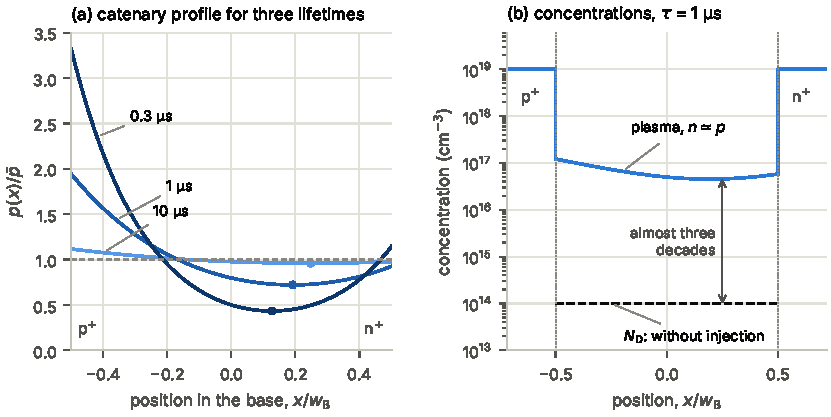
\includegraphics[width=\textwidth]{figures/fig_profile.pdf}
\caption{Plasma in the example base at \SI{\pdExJ}{\ampere\per\centi\metre\squared}. (a) Profile \eqref{eq:catenary} relative to the mean concentration $\bar p = \tau J/(q\wB)$, for three lifetimes: $d/\La = \pdExSlowBeta$, \pdExMidBeta{} and \pdExFastBeta. The point is the minimum, shifted towards the \Np{} emitter. (b) Concentrations on a logarithmic scale for $\tau = \SI{\pdExMidTau}{\micro\second}$: without injection the base has only the electrons of the doping.}
\label{fig:profile}
\end{figure}

\subsection{Drop on the modulated base}
\label{sec:vm}
In high injection the field \eqref{eq:efield} is
\begin{equation}
\Ef = \frac{J}{q\,(\mun+\mup)\,p} - B\,\VT\,\frac{1}{p}\,\dpar{p}{x} .
\label{eq:fieldhl}
\end{equation}
The first term is the ohmic drop on the plasma, whose conductivity $\sigma = q\,(\mun+\mup)\,p$ is to be compared with that of the base without injection, $\sigma_0 = q\,\mun\ND$:
\begin{equation}
\frac{\sigma}{\sigma_0} = \frac{\mun+\mup}{\mun}\,\frac{p}{\ND} \approx \pdSigmaRatio\,\frac{p}{\ND} ,
\end{equation}
that is about \num{\pdExMidSigRatio} at the mean concentration of the example with $\tau = \SI{\pdExMidTau}{\micro\second}$. The second term is the Dember field: where the concentration varies, the electrons would diffuse faster than the holes, and a field holds them back.

The voltage on the base is the integral of the field, $\VM = \int_{-d}^{d}\Ef\,\diff x$. With the profile \eqref{eq:catenary} the integral is calculated in closed form (Appendix~\ref{app:vm}):
\begin{equation}
\frac{\VM}{\VT} = 2\,(1-B^2)\,\frac{\sinh\beta}{\sqrt{1-B^2\tanh^2\beta}}\,\arctan\!\Bigl(\sqrt{1-B^2\tanh^2\beta}\;\sinh\beta\Bigr)
+ B\,\ln\frac{1+B\tanh^2\beta}{1-B\tanh^2\beta} , \quad \beta = \frac{d}{\La} .
\label{eq:vm}
\end{equation}
The first term is the ohmic part, the second the Dember part, $B\,\VT\ln[p(-d)/p(d)]$. Equation \eqref{eq:vm} depends only on $d/\La$ and on the ratio of the mobilities: \emph{it does not depend on the current}. The current provides itself with the conductivity it needs: doubling $J$ doubles the plasma, and the resistance halves. The modulated base does not behave as a resistor, but as a small constant drop in series with the junctions. Equation \eqref{eq:vm} has two limits (Fig.~\ref{fig:vm}a and Table~\ref{tab:vm}).

\emph{Thin base} ($d \ll \La$). The profile is almost flat and
\begin{equation}
\VM \simeq 2\,\VT\left(\frac{d}{\La}\right)^{2} = \frac{\wB^2\,(\mun+\mup)}{4\,\mun\mup\,\tau} ,
\label{eq:vmthin}
\end{equation}
within \SI{\pdVmThinErrOnePct}{\percent} up to $d = \La$. The drop grows with the square of the base width and in inverse proportion to the lifetime. The estimate obtained with a flat profile $p = \bar p$ and the ohmic drop alone [M]~\cite{mohan},
\begin{equation}
\VM \approx \frac{J\,\wB}{q\,(\mun+\mup)\,\bar p} = \frac{\wB^2}{(\mun+\mup)\,\tau} ,
\label{eq:vmflat}
\end{equation}
is the ohmic part of \eqref{eq:vmthin}, that is the fraction $1-B^2$ of the total. With equal mobilities the two coincide; in silicon \eqref{eq:vmflat} is lower by \SI{\pdVmFlatLowPct}{\percent}, the Dember part that even an almost flat profile has.

\emph{Wide base} ($d \gg \La$). The plasma empties in the middle, where the conductivity is lowest, and
\begin{equation}
\VM \simeq \frac{\pi}{2}\,\sqrt{1-B^2}\;\VT\,e^{d/\La} \approx \pdVmAsymCoef\;\VT\,e^{d/\La} .
\label{eq:vmwide}
\end{equation}
The drop grows exponentially with $d/\La$. The asymptote is reached slowly, from above: at $d/\La = 3$ it still exceeds the exact value by \SI{\pdVmAsymErrThreePct}{\percent}. The form $(3\pi/8)\,\VT\,e^{d/\La}$, written for $b = 3$ [M]~\cite{baliga}, is often found in textbooks: it lacks the factor $1/\sqrt{1-B^2}$ of the exact asymptote, and precisely for this reason it is close to the exact value between $d/\La = 2$ and $3$ (within \SI{\pdVmHandErrThreePct}{\percent}).

\begin{table}[htb]
\centering\small
\caption{Drop on the modulated base \eqref{eq:vm} with the mobilities of silicon at \SI{300}{\kelvin}, and deviation of the two limits and of the textbook form.}
\label{tab:vm}
\begin{tabular}{@{}lccccc@{}}
\toprule
$d/\La$ & 0.5 & 1 & 2 & 3 & 4 \\
\midrule
$\VM/\VT$ & \pdVmHalfVt & \pdVmOneVt & \pdVmTwoVt & \pdVmThreeVt & \pdVmFourVt \\
$\VM$ at \SI{300}{\kelvin} [mV] & \pdVmHalfMv & \pdVmOneMv & \pdVmTwoMv & \pdVmThreeMv & \pdVmFourMv \\
Deviation of the thin-base limit \eqref{eq:vmthin} & $\pdVmThinSgnHalf\,\%$ & $\pdVmThinSgnOne\,\%$ & $\pdVmThinSgnTwo\,\%$ & $\pdVmThinSgnThree\,\%$ & $\pdVmThinSgnFour\,\%$ \\
Deviation of the wide-base asymptote \eqref{eq:vmwide} & & & $\pdVmAsymSgnTwo\,\%$ & $\pdVmAsymSgnThree\,\%$ & $\pdVmAsymSgnFour\,\%$ \\
Deviation of the textbook form $(3\pi/8)\,\VT\,e^{d/\La}$ & & & $\pdVmHandSgnTwo\,\%$ & $\pdVmHandSgnThree\,\%$ & $\pdVmHandSgnFour\,\%$ \\
\bottomrule
\end{tabular}
\end{table}

\begin{figure}[htb]
\centering
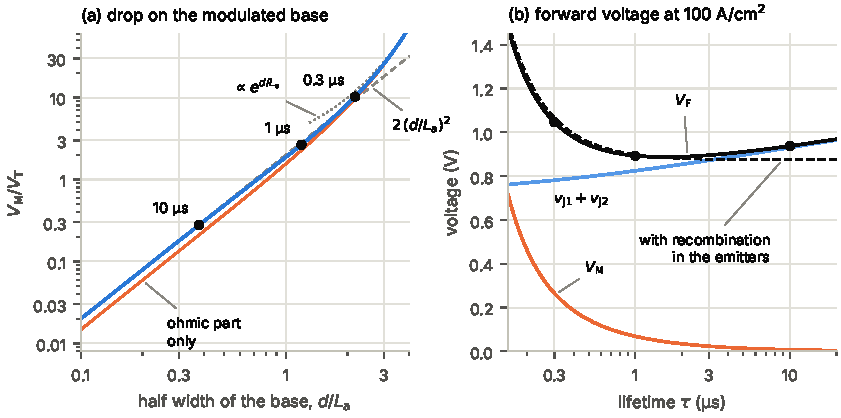
\includegraphics[width=\textwidth]{figures/fig_vm.pdf}
\caption{(a) Drop on the modulated base in units of $\VT$ against $d/\La$: exact expression \eqref{eq:vm}, its ohmic part alone, thin-base limit \eqref{eq:vmthin} (dashed) and wide-base asymptote \eqref{eq:vmwide} (dotted). The points are the three lifetimes of the example. (b) Example base at \SI{\pdExJ}{\ampere\per\centi\metre\squared} against the lifetime, with ideal emitters: sum of the two junction voltages, drop $\VM$ and forward voltage $\VF$. The forward voltage has a flat minimum around $d = \La$. Dashed, $\VF$ with the recombination in the emitters of Sec.~\ref{sec:emitter}.}
\label{fig:vm}
\end{figure}

Equation \eqref{eq:vm} holds as long as its assumptions hold. Between $10^{16}$ and $10^{17}\,\cmc$ carrier-carrier scattering begins to reduce the mobilities, and the drop starts to grow with the current again; the recombination in the emitters (Sec.~\ref{sec:emitter}) makes the plasma grow less than the current, with the same effect; at very low currents, when the plasma falls towards the doping, the modulation is lost. To these terms are added the resistances of the emitters, of the substrate and of the contacts. It is the combination of these effects that gives the real characteristic a resistive slope at high currents.

\subsection{Junction voltages and forward characteristic}
\label{sec:vf}
The terminal voltage is the difference between the quasi-Fermi level of the electrons at the cathode and that of the holes at the anode. In the emitters, which are heavily doped, the quasi-Fermi level of the majority carriers is flat (Sec.~\ref{sec:transport}), and it also crosses the space charge region flat (Sec.~\ref{sec:bias}): $\EFp$ is constant from the anode contact to the edge $x = -d$ of the base, and $\EFn$ from the cathode contact to $x = +d$, even with non-ideal emitters. So $q\,\VF = \EFn(d) - \EFp(-d)$. In the base $n = p$, and by \eqref{eq:qfl} the distance between the two levels is $2\kB T\ln(p/\nint)$ at every point; moreover $\EFp = E_\mathrm{i} - \kB T\ln(p/\nint)$, and the difference of $E_\mathrm{i}$ between the two edges is $q\VM$ by \eqref{eq:potential}. Adding up,
\begin{equation}
\VF = \VT\,\ln\frac{p(-d)\,p(d)}{\nint^2} + \VM .
\label{eq:vfqfl}
\end{equation}
The first term is divided between the two junctions. At the \Pp\Nm{} junction the barrier is lowered by $\vjo$, and the holes at the edge of the base grow by the Boltzmann factor with respect to their equilibrium value $\nint^2/\ND$; at the \Nm\Np{} junction the barrier is lowered by $\vjt$ and the electrons at the edge, equal to the holes, grow with respect to $\ND$:
\begin{equation}
\vjo = \VT\,\ln\frac{p(-d)\,\ND}{\nint^2} , \qquad \vjt = \VT\,\ln\frac{p(d)}{\ND} , \qquad
p(-d)\,p(d) = \nint^2\,e^{(\vjo+\vjt)/\VT} .
\label{eq:vj12}
\end{equation}
The forward voltage is therefore the sum of three contributions,
\begin{equation}
\VF = \vjo + \VM + \vjt .
\label{eq:vfsum}
\end{equation}
The third of \eqref{eq:vj12} is the junction law \eqref{eq:junctionlaw} for the PIN structure: the product is taken between the two edges of the base, and the voltage is the sum $\vj = \vjo + \vjt$ of the two junction voltages. The doping of the base has disappeared: in high injection it no longer has any role in the characteristic. The voltages $\vjo$ and $\vjt$ are the lowerings of the two barriers, and not the separations of the quasi-Fermi levels at the edges of the base, which in high injection are larger (Sec.~\ref{sec:bias}): at $x = -d$ the separation is $q\,\vjo + \kB T\ln[p(-d)/\ND]$. In the example with $\tau = \SI{\pdExMidTau}{\micro\second}$ the two voltages are \SI{\pdExMidVjOne}{\volt} and \SI{\pdExMidVjTwo}{\volt}: the \Nm\Np{} junction contributes one fifth and is not negligible. At the \Pp{} edge the two quasi-Fermi levels are \SI{\pdExMidQflOne}{\electronvolt} apart, against $q\,\vjo = \SI{\pdExMidVjOne}{\electronvolt}$.

\emph{Characteristic.} With the edge concentrations \eqref{eq:edges}, the third of \eqref{eq:vj12} ties the current to the sum of the junction voltages:
\begin{equation}
J = J_\mathrm{HL}\;e^{\vj/(2\VT)} , \qquad J_\mathrm{HL} = \frac{2\,q\,\Da\,\nint}{\La}\,\frac{1}{\sqrt{\coth^2\beta - B^2\tanh^2\beta}} .
\label{eq:jhl}
\end{equation}
The edge concentration grows as $e^{\vj/(2\VT)}$, and with ideal emitters the current grows with it: in high injection the emission coefficient is $\Nem = 2$ (with real emitters it is lower, Sec.~\ref{sec:emitter}). For every decade of current the junction voltage grows by $2\VT\ln 10$, about \SI{120}{\milli\volt} at \SI{300}{\kelvin}, twice as much as in low injection. Since $\VM$ does not depend on the current, the forward voltage is $\VF = 2\VT\ln(J/J_\mathrm{HL}) + \VM$: the drop on the base shifts the characteristic by a constant. A circuit model with a single junction, such as that of Part~II, absorbs it into the saturation current.

\emph{Minimum of the forward voltage.} At fixed current and base width, from \eqref{eq:jhl} and \eqref{eq:vm} the forward voltage depends on the lifetime only through $\beta$:
\begin{equation}
\frac{\VF}{\VT} = 2\,\ln\frac{J\,d}{2\,q\,\Da\,\nint} - 2\ln\beta + \ln\bigl(\coth^2\beta - B^2\tanh^2\beta\bigr) + \frac{\VM(\beta)}{\VT} .
\label{eq:vfbeta}
\end{equation}
For a thin base the three terms that depend on $\beta$ are $-4\ln\beta + \tfrac{8}{3}\beta^2$, with the minimum at $\beta = \sqrt{3}/2 \approx \num{0.87}$; the exact expression has the minimum at $d/\La = \pdVfMinBeta$, whatever the current and the width. The minimum is flat: $\VF$ stays within \SI{10}{\milli\volt} of the minimum for $d/\La$ from \pdVfFlatLo{} to \pdVfFlatHi{} (Fig.~\ref{fig:vm}b). Below the minimum, that is for a smaller $d/\La$ and a longer lifetime (on the right in Fig.~\ref{fig:vm}b, which has the lifetime on the abscissa), $\VM$ is negligible and the voltage is that of the junctions, which grows with the logarithm of the edge concentration: lengthening the lifetime increases the plasma and raises $\VF$ slightly. Above the minimum (on the left in the figure) $\VM$ dominates, and it grows exponentially. A fast diode sits on this branch: it pays in forward voltage what it gains in charge. A lifetime longer than the one that gives $d \approx \La$, on the other hand, is of no use to the conduction and only adds charge to be removed.

\begin{table}[htb]
\centering\small
\caption{Conduction of the example base ($\wB = \SI{\pdExW}{\micro\metre}$, $\ND = \pdExNd\,\cmc$) at \SI{\pdExJ}{\ampere\per\centi\metre\squared} and \SI{300}{\kelvin}, for three lifetimes. Without injection the same base would drop \SI{\pdExDropUni}{\volt}. The last three rows are with the recombination in the emitters, $h_\mathrm{p} = h_\mathrm{n} = \pdHem\,\si{\centi\metre^4\per\second}$. The column with $\tau = \SI{\pdExSlowTau}{\micro\second}$ and ideal emitters is a limiting case: at its mean concentration the Auger lifetime, about \SI{\pdExSlowTauAuger}{\micro\second}, is shorter than $\tau$, and carrier-carrier scattering has already reduced the mobilities. With the recombination in the emitters the plasma falls to $\pdExSlowEmPbar\,\cmc$: the Auger lifetime is again much longer than $\tau$, while the reduction of the mobilities by carrier-carrier scattering is left out of the numbers of the table, as in the other two columns (assumption 5, Sec.~\ref{sec:ambipolar}).}
\label{tab:conduction}
\begin{tabular}{@{}llccc@{}}
\toprule
Lifetime $\tau$ & & \SI{\pdExSlowTau}{\micro\second} & \SI{\pdExMidTau}{\micro\second} & \SI{\pdExFastTau}{\micro\second} \\
\midrule
Diffusion length $\La$; $d/\La$ & & \SI{\pdExSlowLa}{\micro\metre}; \pdExSlowBeta & \SI{\pdExMidLa}{\micro\metre}; \pdExMidBeta & \SI{\pdExFastLa}{\micro\metre}; \pdExFastBeta \\
Mean concentration $\bar p$ [\si{\centi\metre^{-3}}] & \eqref{eq:qf} & $\pdExSlowPbar$ & $\pdExMidPbar$ & $\pdExFastPbar$ \\
\Pp{} edge, $p(-d)$ [\si{\centi\metre^{-3}}] & \eqref{eq:edges} & $\pdExSlowPl$ & $\pdExMidPl$ & $\pdExFastPl$ \\
\Np{} edge, $p(d)$ [\si{\centi\metre^{-3}}] & \eqref{eq:edges} & $\pdExSlowPr$ & $\pdExMidPr$ & $\pdExFastPr$ \\
Minimum [\si{\centi\metre^{-3}}] & & $\pdExSlowPmin$ & $\pdExMidPmin$ & $\pdExFastPmin$ \\
Stored charge $\tau J$ [\si{\micro\coulomb\per\centi\metre\squared}] & \eqref{eq:qf} & \pdExSlowQs & \pdExMidQs & \pdExFastQs \\
Mean conductivity relative to $\sigma_0$ & & \pdExSlowSigRatio & \pdExMidSigRatio & \pdExFastSigRatio \\
\addlinespace
Drop on the base $\VM$ [mV] & \eqref{eq:vm} & \pdExSlowVm & \pdExMidVm & \pdExFastVm \\
\quad of which Dember part [mV] & & \pdExSlowVmDem & \pdExMidVmDem & \pdExFastVmDem \\
\quad flat-profile estimate [mV] & \eqref{eq:vmflat} & \pdExSlowVmFlat & \pdExMidVmFlat & \pdExFastVmFlat \\
Junction voltages $\vjo$; $\vjt$ [V] & \eqref{eq:vj12} & \pdExSlowVjOne; \pdExSlowVjTwo & \pdExMidVjOne; \pdExMidVjTwo & \pdExFastVjOne; \pdExFastVjTwo \\
Forward voltage $\VF$ [V] & \eqref{eq:vfsum} & \pdExSlowVf & \pdExMidVf & \pdExFastVf \\
\addlinespace
Current that recombines in the emitters & \eqref{eq:emitterbal} & \SI{\pdExSlowEmPct}{\percent} & \SI{\pdExMidEmPct}{\percent} & \SI{\pdExFastEmPct}{\percent} \\
Effective lifetime $Q/i$ [\si{\micro\second}] & \eqref{eq:taueff} & \pdExSlowEmTauEff & \pdExMidEmTauEff & \pdExFastEmTauEff \\
Forward voltage $\VF$ [V] & & \pdExSlowEmVf & \pdExMidEmVf & \pdExFastEmVf \\
\bottomrule
\end{tabular}
\end{table}

\subsection{Recombination in the emitters and effective lifetime}
\label{sec:emitter}
A real emitter is not ideal: the base in turn injects minority carriers into it, electrons into the \Pp{} emitter and holes into the \Np{} emitter, which recombine there. By the junction law \eqref{eq:junctionlaw} the product $np$ is the same on the two sides of the space charge region; at the edge of the base it is $p^2$, so the concentration of the minority carriers injected into the emitter is $p^2/\NA$, and their diffusion current is proportional to $p^2$. The boundary conditions \eqref{eq:bc} become \cite{schlangenotto1969}, [M]~\cite{lutz}
\begin{equation}
\Jn(-d) = q\,h_\mathrm{p}\,p^2(-d) , \qquad \Jp(d) = q\,h_\mathrm{n}\,p^2(d) ,
\label{eq:bcem}
\end{equation}
where $h_\mathrm{p}$ and $h_\mathrm{n}$ are the recombination parameters of the two emitters. In a uniform emitter $h = D_\mathrm{E}/(L_\mathrm{E}\,N_\mathrm{E})$, with the diffusion constant and the diffusion length of the minority carriers in the emitter and its doping; in a real emitter the band-gap narrowing and the Auger recombination increase it, and the typical values are of the order of \SIrange[range-exponents=combine-bracket]{1e-14}{3e-14}{\centi\metre^4\per\second} [M]~\cite{lutz}.

Integrating \eqref{eq:diffusion} in the steady state over the base, with \eqref{eq:jnjp} at the two edges, the balance of the current is
\begin{equation}
J = \frac{q\,\wB\,\bar p}{\tau} + q\,h_\mathrm{p}\,p^2(-d) + q\,h_\mathrm{n}\,p^2(d) :
\label{eq:emitterbal}
\end{equation}
the current feeds the recombination in the base and that in the two emitters. The charge is no longer $\tau\,\IF$. The \emph{effective lifetime} is defined as
\begin{equation}
\tau_\mathrm{eff} = \frac{Q}{i} = \tau\left(1 - \frac{\Jn(-d) + \Jp(d)}{J}\right) ,
\label{eq:taueff}
\end{equation}
which is shorter than $\tau$ and \emph{depends on the current}: the recombination in the base grows as $p$, that in the emitters as $p^2$. For the example base with $\tau = \SI{\pdExMidTau}{\micro\second}$ and $h_\mathrm{p} = h_\mathrm{n} = \pdHem\,\si{\centi\metre^4\per\second}$, the profile that satisfies \eqref{eq:bcem} gives \SI{\pdEmJLoPct}{\percent} of the current in the emitters at \SI{\pdEmJLo}{\ampere\per\centi\metre\squared}, \SI{\pdEmJMidPct}{\percent} at \SI{\pdEmJMid}{\ampere\per\centi\metre\squared} and \SI{\pdEmJHiPct}{\percent} at \SI{\pdEmJHi}{\ampere\per\centi\metre\squared}; the effective lifetime falls from \SI{\pdEmJLoTauEff}{\micro\second} to \SI{\pdEmJMidTauEff}{\micro\second} and \SI{\pdEmJHiTauEff}{\micro\second}. With a base lifetime of \SI{\pdExSlowTau}{\micro\second} the emitters take \SI{\pdExSlowEmPct}{\percent} of the current and the effective lifetime is \SI{\pdExSlowEmTauEff}{\micro\second} (Table~\ref{tab:conduction}): in a diode with a long lifetime it is the emitters, not the base, that set the charge. There are five consequences.
\begin{itemize}
\item The stored charge grows less than the current; when the emitters dominate, it grows as $\sqrt{J}$.
\item The drop on the base is no longer independent of the current: the plasma grows less than $J$, and $\VM$ rises. Together with carrier-carrier scattering it is the origin of the resistive part of the characteristic at high current. As a result the forward voltage is higher where $\VM$ prevails and lower with a long lifetime, where the junction voltages fall more than $\VM$ rises (Table~\ref{tab:conduction}).
\item The characteristic \eqref{eq:jhl} changes as well. The current that recombines in the base grows as $e^{\vj/(2\VT)}$, the one that recombines in the emitters, $J_\mathrm{E} = \Jn(-d) + \Jp(d)$, as $e^{\vj/\VT}$: the sum of the junction voltages grows by about $2\VT/(1 + J_\mathrm{E}/J)$ per unit of $\ln J$, that is with an emission coefficient between 2 and 1. In the example at \SI{\pdExJ}{\ampere\per\centi\metre\squared} the exact profile gives \num{\pdExMidEmSlopeVj}\,$\VT$ with $\tau = \SI{\pdExMidTau}{\micro\second}$ and \num{\pdExSlowEmSlopeVj}\,$\VT$ with \SI{\pdExSlowTau}{\micro\second}. At the terminals the slope is higher, \num{\pdExMidEmSlopeVf}\,$\VT$ and \num{\pdExSlowEmSlopeVf}\,$\VT$, because $\VM$ rises in the meantime.
\item The lifetime that a circuit sees depends on the state of the plasma. A fast current ramp, which leaves more charge in the base, meets a shorter effective lifetime than a slow ramp. A model with a constant lifetime cannot follow it: this is the main limit of the model of Part~II (Sec.~\ref{sec:slope}).
\item The efficiency of the emitters is a design lever: a weak emitter keeps the plasma low on its own side without touching the lifetime of the base (Sec.~\ref{sec:emittereff}).
\end{itemize}

\subsection{Temperature}
\label{sec:temperature}
The forward characteristic has two parts with opposite temperature coefficients.

\emph{Junction voltages.} At constant current the edge concentrations are set by the current, and in \eqref{eq:vj12} the temperature enters through $\VT$ and $\nint$. With \eqref{eq:ni}, neglecting the temperature dependence of the lifetime and of the diffusion constants,
\begin{equation}
\frac{\diff\vj}{\diff T} \approx \frac{\vj - E_\mathrm{g0}/q - 3\,\VT}{T} :
\label{eq:tc}
\end{equation}
\SI{-\pdTcLo}{\milli\volt\per\kelvin} for $\vj = \SI{\pdTcVjLo}{\volt}$ and \SI{-\pdTcHi}{\milli\volt\per\kelvin} for $\vj = \SI{\pdTcVjHi}{\volt}$, the sum of the two junction voltages of the example. The coefficient is negative, because $\nint$ grows with the temperature, and it decreases in absolute value as the voltage grows: in high injection by $2\,(\kB/q)\ln 10 \approx \SI{0.4}{\milli\volt\per\kelvin}$ for every decade of current. The same relation holds in low injection, with half of this variation.

\emph{Base and resistive parts.} The drop on the base \eqref{eq:vmthin} is inversely proportional to the mobilities, which fall with the temperature (Sec.~\ref{sec:ambipolar}: about as $T^{-2.4}$ for the electrons and $T^{-2.2}$ for the holes, whose mobility weighs more here), and to the lifetime, which rises: the first effect increases it, the second reduces it, and the result depends on the technology of the lifetime control. The resistances of the emitters and of the contacts grow with the temperature.

At low current the junction prevails and the temperature coefficient of $\VF$ is negative; at high current the base and the resistive parts prevail and it becomes positive. The characteristics at two temperatures cross at one point (\emph{crossover}). A positive coefficient at the working current stabilises the sharing of the current between devices in parallel; a diode with a long lifetime and efficient emitters, that is with a small $d/\La$ and a small $\VM$, has the crossover at high currents and has to be checked on the datasheet before it is put in parallel [M]~\cite{lutz}.
%=====================================================================
\part{Charge dynamics and reverse recovery}

\section{The reverse recovery: phenomenon and datasheet quantities}
\label{sec:datasheet}
The stored charge $\QF = \tau\,\IF$ that makes the base conductive (Sec.~\ref{sec:catenary}) has to be removed before the diode can sustain a reverse voltage. As long as plasma remains next to the \Pp\Nm{} junction, the junction stays in forward bias and the diode conducts in the reverse direction as well: this is the \emph{reverse recovery}. This section describes the phenomenon and the quantities with which the datasheet measures it; the following sections describe it with one charge (Sec.~\ref{sec:chargecontrol}) and with two (Sec.~\ref{sec:model}).

\subsection{The turn-off sequence}
\label{sec:sequence}
The turn-off of a diode always takes place in a circuit with a series inductance: the commutation inductance of a converter, or the leakage inductance of a transformer. Figure~\ref{fig:commcell} shows the two circuits to which this document refers. In the \emph{commutation cell} (a) an ideal switch applies the reverse voltage $\VR$ through the inductance $\Ls$, and the diode current falls with the slope $a = \VR/\Ls$: it is the test circuit of the datasheets and that of a line-commutated converter. In the \emph{switching leg} (b) the slope is imposed by the switch that turns on, through its drive, and the drop $\Ls a$ on the stray inductance is only a part of the voltage $\Vdc$.

\begin{figure}[htb]
\centering
\begin{circuitikz}[scale=0.9, transform shape]
\ctikzset{bipoles/length=1.0cm}
% (a) commutation cell
\node[anchor=west] at (-0.9,4.2) {(a)};
\draw (0,0) to[american voltage source, invert, l=$\VR$] (0,3.2) to[closing switch, l={$t=0$}] (1.7,3.2) to[L, l=$\Ls$] (3.4,3.2) -- (6.4,3.2);
\draw (3.4,0) to[D*, l=D, *-*] (3.4,3.2);
\draw (4.9,3.2) to[R, l=$\Rsn$, *-] (4.9,1.6) to[C, l=$\Csn$, -*] (4.9,0);
\draw (6.4,3.2) to[american current source, l=$\IF$] (6.4,0);
\draw (0,0) -- (6.4,0);
\draw[-{Latex[length=2mm]}] (3.05,0.35) -- (3.05,0.95) node[midway, left]{$i$};
% (b) switching leg
\begin{scope}[xshift=9.6cm]
\node[anchor=west] at (-0.9,4.2) {(b)};
\draw (0,0) to[american voltage source, invert, l=$\Vdc$] (0,3.2) to[L, l=$\Ls$] (2.4,3.2) -- (4.6,3.2);
\draw (2.4,1.6) to[D*, l_=D, *-*] (2.4,3.2);
\draw (4.6,3.2) to[american current source, l=$I_\mathrm{L}$] (4.6,1.6) -- (2.4,1.6);
\draw (2.4,1.6) to[closing switch, l=S] (2.4,0);
\draw (0,0) -- (2.4,0);
\draw[-{Latex[length=2mm]}] (2.05,2.05) -- (2.05,2.65) node[midway, left]{$i$};
\end{scope}
\end{circuitikz}
\caption{(a) Commutation cell: the diode carries the current $\IF$ of the load; at $t=0$ the switch applies the voltage $\VR$ in reverse through the inductance $\Ls$, and the diode current falls with the slope $a = \VR/\Ls$. An RC snubber may sit across the diode. (b) Switching leg: the freewheeling diode D carries the current $I_\mathrm{L}$ of the load; the switch S, as it turns on, takes it over with a slope set by its drive, and $\Ls$ is the stray inductance of the loop.}
\label{fig:commcell}
\end{figure}

Figure~\ref{fig:recovery} shows the qualitative waveforms of the current and of the voltage. Four phases can be distinguished.
\begin{enumerate}
\item \emph{Conduction.} The diode carries $\IF$ with the forward voltage $\VF$; the base contains the plasma of the catenary \eqref{eq:catenary} and the stored charge $\tau\,\IF$.
\item \emph{Ramp.} The circuit brings the current to zero at the rate $a$. The charge of the base does not follow: it decreases only by recombination, with the time constant $\tau$, and at the current zero a part of it remains, the larger the shorter the ramp is against $\tau$ (Sec.~\ref{sec:ccsolutions}).
\item \emph{Reverse current with the junction still conducting.} The current reverses and keeps growing in magnitude with the same slope. As long as there is plasma at the edges of the base, the two junctions stay in forward bias: the diode voltage is still a small forward voltage, although the current is reversed, and the diode behaves as a short circuit. The reverse current extracts the plasma from both sides, the holes towards the \Pp{} emitter and the electrons towards the \Np{} emitter: by the boundary conditions \eqref{eq:bc} the gradient at the \Pp\Nm{} edge is $b \approx 3$ times that at the \Nm\Np{} edge, so the anode side empties about three times faster.
\item \emph{Blocking and tail.} When the concentration at the \Pp\Nm{} edge falls to zero, the junction can no longer supply the current that the circuit asks for: a space charge region forms, the diode takes up voltage and the reverse current reaches the peak $\Irr$. In the cell of Fig.~\ref{fig:commcell}a the peak is the instant at which the reverse voltage of the diode, $v_\mathrm{R} = -v$, equals $\VR$, because $\Ls\,\diff i/\diff t = v_\mathrm{R} - \VR$ vanishes there. The residual plasma, which in a base that is not wide against $\La$ lies towards the cathode (Sec.~\ref{sec:onenumber}), keeps supplying current while it is removed by recombination, by diffusion to the edges and by the advance of the space charge region: this is the \emph{tail}. In the tail the current decreases in magnitude, and the inductance adds its voltage to that of the circuit: the reverse voltage exceeds $\VR$ and reaches a peak, which without capacitance across the diode is the $\Vrm$ of \eqref{eq:vrm} and with a capacitance changes (Sec.~\ref{sec:energy}).
\end{enumerate}

\begin{figure}[htb]
\centering
\begin{tikzpicture}[x=1.3cm, y=1.5cm, >={Latex[length=2mm]}, font=\small]
% phases
\foreach \x in {1,2.25,3.156} \draw[gray!70, densely dotted] (\x,-3.4) -- (\x,1.5);
\node at (0.5,1.38) {1}; \node at (1.62,1.38) {2}; \node at (2.7,1.38) {3}; \node at (4.6,1.38) {4};
% --- current
\fill[gray!25] (2.25,0) -- (3.0,-0.6) .. controls (3.1,-0.68) and (3.2,-0.68) .. (3.35,-0.6)
   -- plot[domain=3.35:8.0, samples=60] (\x,{-0.6*exp(-(\x-3.35)/0.9)}) -- (8.0,0) -- cycle;
\draw[->] (0,0) -- (8.5,0) node[right] {$t$};
\draw[->] (0,-0.9) -- (0,1.3) node[above] {$i$};
\draw[thick] (0,1) -- (1,1) -- (3.0,-0.6) .. controls (3.1,-0.68) and (3.2,-0.68) .. (3.35,-0.6)
   -- plot[domain=3.35:8.0, samples=60] (\x,{-0.6*exp(-(\x-3.35)/0.9)});
\node[left] at (0,1) {$\IF$};
\node[anchor=west, fill=white, inner sep=1.5pt] (slope) at (0.1,0.45) {$\diff i/\diff t = -a$};
\draw[->] (slope.east) -- (1.66,0.47);
\draw[<->] (3.156,0) -- (3.156,-0.66);
\node[right] at (3.17,-0.3) {$\Irr$};
\node (qrr) at (5.0,-0.6) {$\Qrr$};
\draw[thin] (qrr.north west) -- (3.9,-0.17);
\draw[<->] (2.25,0.16) -- (3.156,0.16) node[midway, above] {$\ta$};
\draw[<->] (3.156,0.16) -- (5.0,0.16) node[midway, above] {$\tb$};
\draw[gray!70, densely dotted] (5.0,-0.2) -- (5.0,0.75);
\draw[<->] (2.25,0.62) -- (5.0,0.62) node[midway, above] {$\trr$};
% --- reverse voltage
\begin{scope}[yshift=-4.6cm]
\draw[->] (0,0) -- (8.5,0) node[right] {$t$};
\draw[->] (0,-0.25) -- (0,1.55) node[above] {$v_\mathrm{R} = -v$};
\draw[gray, dashed] (0,0.75) -- (8.2,0.75);
\node[left] at (0,0.75) {$\VR$};
\draw[thick] (0,-0.06) -- (2.8,-0.06) plot[smooth, tension=0.55] coordinates {(2.8,-0.06) (2.95,0.04) (3.06,0.38) (3.156,0.75) (3.27,1.08) (3.42,1.24) (3.6,1.2) (3.9,1.05) (4.4,0.9) (5.2,0.8) (6.2,0.76) (8.0,0.75)};
\node[below] at (1.4,-0.06) {$-\VF$};
\draw[<->] (3.42,0) -- (3.42,1.24);
\node[right] at (3.6,1.3) {$\Vrm$};
\end{scope}
\end{tikzpicture}
\caption{Qualitative waveforms of the turn-off of a PIN diode on a current ramp: current and reverse voltage $v_\mathrm{R} = -v$. The numbers mark the phases described in the text; the boundary between phases 3 and 4 is drawn at the peak of the current, shortly after the start of blocking. The grey area is the recovered charge. The end of the recovery, and therefore $\tb$ and $\trr$, needs a convention (Sec.~\ref{sec:rrdata}).}
\label{fig:recovery}
\end{figure}

Three remarks prepare the sections that follow. The first: the reverse current is not a defect of the junction but the removal of a charge, and its size depends on how much charge the ramp has left in the base, not on the static charge. The second: the blocking instant is decided by the concentration at \emph{one edge}, not by the total charge; this is why a single charge is not enough to describe the recovery, and why the shape of the profile matters as much as its integral. The third: in the tail it is the diode that imposes the current and the circuit that is subjected to it, and everything that is dangerous in the recovery (overvoltage, oscillations, dynamic avalanche) happens there.
\subsection{The recovery quantities}
\label{sec:rrdata}
In the recovery test the diode first carries the forward current $\IF$. The circuit then forces the current down at a constant rate $a = -\diff i/\diff t$, through zero and into the reverse direction (Fig.~\ref{fig:waveform}a, which shows the waveform of the two-charge model of Sec.~\ref{sec:model}). The reverse current rises to the peak $\Irr$, which it reaches at the time $\ta$ after the current zero; the diode then takes up the reverse voltage $\VR$ and the current falls back to zero in the time $\tb$. The datasheet gives some of the following quantities, with the test conditions $\IF$, $a$, $\VR$ and the junction temperature.
\begin{itemize}
\item \emph{Peak reverse recovery current} $\Irr$ ($I_\mathrm{rrm}$ in IEC~60747-2 \cite{iec60747}, 3.3.10; $I_\mathrm{RM}$ or $I_\mathrm{RR}$ in many datasheets).
\item \emph{Recovered charge} $\Qrr$ ($Q_\mathrm{r}$ in \cite{iec60747}, 3.5.5; also $Q_\mathrm{S}$): the integral of the reverse current from the current zero. The standard ends the integral at the instant at which the current has fallen to \SI{\lmPEndPct}{\percent} of the peak, and notes that the charge includes components due to both carrier storage and junction capacitance (3.5.5, Note~2). Some datasheets call it stored charge; in this document the stored charge is the charge present in the base, of which the recovered charge is a part.
\item \emph{Reverse recovery time} $\trr = \ta + \tb$ (\cite{iec60747}, 3.5.2), from the current zero to the end of the recovery. The current approaches zero asymptotically, so the end needs a convention. The standard draws a straight line through two points A and B of the falling current and takes the instant at which the line reaches zero; A is often specified at \SI{90}{\percent} and B at \SI{25}{\percent} of the peak (3.5.2, Note~5). The same construction is in \cite{an6481}, Sec.~2.1. Other documents take the instant at which the current has fallen to a fraction of the peak: \SI{10}{\percent} in the documentation of the simulators \cite{mathworks,plecs}, a fraction $k$, usually \num{0.25}, in \cite{an5028}. The standard names the two parts of $\trr$ rise time and fall time (3.5.3, 3.5.4).
\item \emph{Softness}: the ratio $\tb/\ta$ (\cite{an6481}, Sec.~2.1; \cite{an5028}), or a ratio of the two slopes of the reverse current, before and after the peak. The terms soft and snappy are defined in Sec.~\ref{sec:softsnappy}.
\end{itemize}
Rectifier diodes for line frequency usually come with the maximum $\Qrr$ and $\Irr$ at the maximum junction temperature and at a slope of a few \Aus, and with curves of the two quantities against the slope. Fast diodes come with typical $\Irr$, $\Qrr$ and $\trr$ at two temperatures and at hundreds or thousands of \Aus, with curves against the forward current and the slope.

\begin{figure}[htb]
\centering
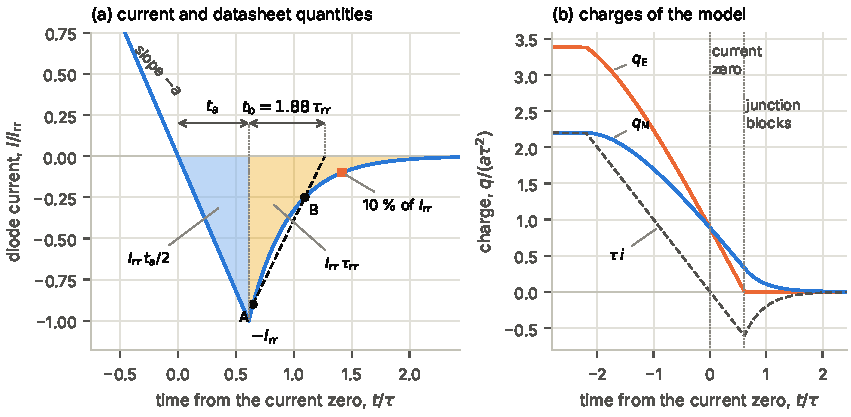
\includegraphics[width=\textwidth]{../lauritzen_ma_datasheet_conversion/figures/fig_waveform.pdf}
\caption{Turn-off of the two-charge model (Sec.~\ref{sec:model}) on a current ramp ($\rho = \taurr/\tau = \lmFigRho$, $\IF/(a\tau) = \lmFigLam$). (a) Current and datasheet quantities: the triangle of charge $\Irr\ta/2$, the tail of charge $\Irr\taurr$, the straight line through the points A (\SI{90}{\percent}) and B (\SI{25}{\percent}) that defines $\tb$, and the point at \SI{10}{\percent}. (b) The two charges of the model and, dashed, $\tau i$: the middle charge $\qM$ follows the current with a delay, the edge charge $\qE$ reaches zero after the current, and at that instant the junction blocks.}
\label{fig:waveform}
\end{figure}

\subsection{Forward characteristic in the datasheet}
For a rectifier diode the datasheet gives the forward voltage at one current and a straight-line approximation of the characteristic at the maximum temperature,
\begin{equation}
v \approx \VTo + \rT\, i ,
\label{eq:line}
\end{equation}
with the threshold voltage $\VTo$, not to be confused with the thermal voltage $\VT$, and the slope resistance $\rT$. The line crosses the real characteristic at two currents, which the datasheet states or which are implied by the range of validity of the line. For a fast diode the datasheet gives the forward voltage at the rated current and a curve at two temperatures.

\subsection{Blocking state in the datasheet}
The datasheet gives the reverse current $\Irrm$ at the repetitive peak reverse voltage $\Vrrm$ and at the maximum temperature, as a maximum; it is a static current, not to be confused with the recovery peak, which the standard denotes by $I_\mathrm{rrm}$. A junction capacitance is given for small and fast diodes, at a low reverse voltage; for large rectifier diodes it is usually not given.
\subsection{Soft and snappy}
\label{sec:softsnappy}
The way the current falls back to zero after the peak decides the overvoltage. In the tail $\diff i/\diff t > 0$, and the reverse voltage of the diode is $v_\mathrm{R} = \VR + \Ls\,\diff i/\diff t$: the overvoltage is proportional to the rate at which the tail dies out.

A diode is \emph{soft} if plasma remains in the base until the space charge region has reached the extent that corresponds to the applied voltage: the current then decays with the time constant of the residual plasma, and the overvoltage is limited. It is \emph{snappy} if the plasma is exhausted while a significant reverse current still flows: the current is interrupted in a very short time (\emph{snap-off}), the overvoltage is high, to the point of bringing the reverse voltage above the $\Vrrm$ of the diode, and the inductance oscillates with the junction capacitance of the diode, with the electromagnetic interference (EMI) that follows.

Rather than the two measures of the softness of Sec.~\ref{sec:rrdata}, this document prefers the ratio $s$ of the charge of the tail to that of the triangle, \eqref{eq:soft}; in the two-charge model, on a long ramp, it is $2\TM/\tau$, where the transit time $\TM$ of the model is of the order of the diffusion time over the half width of the base, $d^2/(3\Da)$ (Secs.~\ref{sec:lumped} and~\ref{sec:onenumber}). It has to be read for what it is: $s$ measures the shape of a diffusion tail, and none of these measures predicts the snap-off. The two-charge model does not contain it, because its tail is always an exponential; and at a fixed geometry $2\TM/\tau$ grows when the lifetime is reduced, without a real diode becoming softer because of it.

The conditions that favour the snap-off can be read from the physics of Part~I [M]~\cite{lutz}.
\begin{itemize}
\item \emph{Thin base.} In a punch-through base or one with a field stop the space charge region reaches the end of the base at the voltage $q\ND\wB^2/(2\varepsilon)$, \SI{\pdExVrt}{\volt} for the example base (\SI{\pdExW}{\micro\metre}, $\pdExNd\,\cmc$). If the applied voltage exceeds it, the space charge region sweeps the whole base and the residual plasma has nowhere to stay.
\item \emph{High voltage}, for the same reason; \emph{low current} and \emph{low temperature}, because the stored charge is smaller; \emph{steep slope} and \emph{high inductance}, because the voltage rises earlier and higher.
\end{itemize}
A rule for checking a diode follows: the losses, $\Qrr$ and $\Irr$ are to be taken at the maximum junction temperature and at the rated current; the overvoltage and the softness are to be checked also at low temperature and at low current, of the order of one tenth of the rated one, with the highest voltage.

For the recovery the distribution of the plasma therefore matters as well as its quantity. The plasma next to the \Pp\Nm{} junction has to be removed before the junction can block, and sets $\Irr$; the plasma on the cathode side feeds the tail, and sets the softness. The technologies of Sec.~\ref{sec:technology} act on this distribution.

\subsection{Dynamic avalanche}
\label{sec:dynaval}
During the recovery the space charge region forms while the reverse current crosses it. In it the current is carried by holes that travel towards the \Pp{} emitter at a velocity close to the saturation velocity, $v_\mathrm{sat} \approx \SI{e7}{\centi\metre\per\second}$ [M]~\cite{sze}, with the concentration
\begin{equation}
p = \frac{J}{q\,v_\mathrm{sat}} .
\label{eq:pdyn}
\end{equation}
Their charge adds to that of the donors, and \eqref{eq:poisson} gives
\begin{equation}
\dpar{\Ef}{x} = \frac{q}{\varepsilon}\,(\ND + p) .
\label{eq:dynfield}
\end{equation}
The base behaves as if its doping were $\ND + p$: the field has a steeper gradient and reaches the critical value at a lower voltage. At \SI{\pdDynJLo}{\ampere\per\centi\metre\squared} \eqref{eq:pdyn} gives $p = \pdDynPLo\,\cmc$, \SI{\pdDynPctLo}{\percent} of the doping of the example base: with \eqref{eq:ecrit} and a triangular field the critical value is reached at about \SI{\pdDynVbrLo}{\volt}, against the \SI{\pdBlkVC}{\volt} of the same doping without current (Table~\ref{tab:blocking}) and the static \SI{\pdExVbr}{\volt} of the example base, which is punch-through. At \SI{\pdDynJHi}{\ampere\per\centi\metre\squared} it is reached at about \SI{\pdDynVbrHi}{\volt}.

This is the \emph{dynamic avalanche}: impact ionisation at voltages well below the static breakdown voltage, present only while the reverse current flows. A moderate dynamic avalanche is self-limiting, because the generated electrons cross the space charge region and partly compensate the charge of the holes; a strong one can concentrate the current into filaments and destroy the diode [M]~\cite{lutz}. It is what limits the product of reverse current and voltage during the recovery, that is the \emph{safe operating area} (SOA) of the diode in reverse recovery, which some datasheets report, and with it the slope allowed at the highest voltages.

\subsection{Forward recovery}
\label{sec:forwardrec}
At the turn-on of the diode the opposite phenomenon occurs. If the current rises faster than the plasma can form, the base is still the one without injection, with the resistance $R_\mathrm{B} = \wB/(q\,\mun\,\ND)$ of \eqref{eq:runi}: \SI{\pdExRuni}{\ohm\centi\metre\squared} for the example base, that is \SI{\pdExDropUni}{\volt} at \SI{\pdExJ}{\ampere\per\centi\metre\squared}, and \SI{\pdTgtDrop}{\volt} for the \SI{\pdTgtV}{\kilo\volt} non-punch-through base of Sec.~\ref{sec:why}. These are the upper limits, for a current applied as a step. The diode voltage therefore has a peak $V_\mathrm{FRM}$ (\emph{forward recovery}), which can be tens or hundreds of volts, and then falls to $\VF$ while the plasma fills the base. The characteristic time is that of the diffusion of the plasma in the base, of the order of the transit time $d^2/(3\Da)$ of Sec.~\ref{sec:lumped} (\SI{\pdExTmPar}{\nano\second} for the example base), not of the lifetime. The peak grows with the slope, with the base width, that is with the voltage class, and with the temperature, because the mobility falls [M]~\cite{lutz}; the inductive drop of the package adds to it.

The forward recovery matters where a diode has to take up current quickly: in clamp and snubber diodes, whose peak voltage adds to the one they should limit, and in the freewheeling diode at the turn-off of the switch. The two-charge model does not reproduce it (Sec.~\ref{sec:otherlimits}).
%=====================================================================
\section{The charge-control model}
\label{sec:chargecontrol}
The simplest model of the dynamics of the diode describes the whole base with a single number, the stored charge $Q = qA\int p\,\diff x$. It follows from the ambipolar diffusion equation with no further approximation, and retains from it what matters most in the time domain: the delay with which the charge follows the current. It is also the charge model of the diode of SPICE, with the parameter \texttt{TT} in place of $\tau$ (Sec.~\ref{sec:others}).

\subsection{Derivation}
\label{sec:ccderiv}
Integrate \eqref{eq:diffusion} over the base, from $-d$ to $+d$, and multiply by $qA$:
\begin{equation}
\frac{\diff Q}{\diff t} = q\,A\,\Da\left[\dpar{p}{x}\right]_{-d}^{+d} - \frac{Q}{\tau} .
\label{eq:integrated}
\end{equation}
The first term is the flow of plasma that enters from the two edges. With the boundary conditions \eqref{eq:bc} of the ideal emitters it is $q A \Da\,J\,[1/(2q\Dn) + 1/(2q\Dp)] = A\,J = i$, by \eqref{eq:da}. This gives the \emph{charge-control equation}
\begin{equation}
\frac{\diff Q}{\diff t} = i - \frac{Q}{\tau} .
\label{eq:cc}
\end{equation}
The current feeds the charge, recombination consumes it. In the steady state every injected carrier recombines in the base, and $i = Q/\tau$: the current of a PIN diode is not a transit of carriers from one terminal to the other, but the feeding of a recombination.

\emph{In one line.} The same result is obtained by integrating over the base the continuity equation of the holes \eqref{eq:contp}, with $U = p/\tau$: $\diff Q/\diff t = A\,[\Jp(-d) - \Jp(+d)] - Q/\tau$. With ideal emitters $\Jp(-d) = J$ and $\Jp(+d) = 0$, and it is again \eqref{eq:cc}. This route shows that the equation does not require high injection, quasi-neutrality, a uniform doping, constant mobilities or a shape of the profile. It requires three things:
\begin{itemize}
\item \emph{ideal emitters}. With the recombination in the emitters of Sec.~\ref{sec:emitter} the balance becomes
\begin{equation}
\frac{\diff Q}{\diff t} = i - \frac{Q}{\tau} - q\,A\,\bigl[h_\mathrm{p}\,p^2(-d) + h_\mathrm{n}\,p^2(d)\bigr] ,
\label{eq:ccem}
\end{equation}
and the static charge is $\tau_\mathrm{eff}\,\IF$ with the effective lifetime \eqref{eq:taueff}, which falls as the current grows: $\QF = \tau\,\IF$ is an upper limit;
\item \emph{linear recombination} with a single $\tau$. The Shockley--Read--Hall lifetime goes from $\tau_\mathrm{p0}$ in low injection to $\tau_\mathrm{p0} + \tau_\mathrm{n0}$ in high injection (Sec.~\ref{sec:lifetime}): \eqref{eq:cc} holds across the two regimes only with a $\tau$ that depends on the injection level;
\item that $i$ is the conduction current. When the junction blocks, the current of the junction capacitance, $\Cj\,\diff v/\diff t$, is added to the terminal current.
\end{itemize}

\subsection{Notable solutions}
\label{sec:ccsolutions}
\emph{Steady state.} With $\diff Q/\diff t = 0$ \eqref{eq:cc} gives \eqref{eq:qf}, $\QF = \tau\,\IF$. With the drop on the thin base \eqref{eq:vmthin} the product
\begin{equation}
\VM\,\QF = \frac{\wB^2\,(\mun+\mup)}{4\,\mun\,\mup}\;\IF
\label{eq:tradeoff}
\end{equation}
does not depend on the lifetime: it is the fundamental trade-off of the bipolar diode. For a given base, every reduction of the stored charge is paid for with a proportional increase of the drop on the base; for the example base $\VM\,\tau = \SI{\pdExVmTau}{\milli\volt\micro\second}$. The only way to reduce both is a thinner base.

\emph{Open circuit.} If the current is interrupted, $i = 0$ and
\begin{equation}
Q(t) = \QF\,e^{-t/\tau} :
\label{eq:opencircuit}
\end{equation}
the charge disappears by recombination alone. Without current the gradients at the edges are zero, the profile flattens and the concentration at the edges follows the charge; with the junction law in high injection, $p \propto e^{\vj/(2\VT)}$ (Sec.~\ref{sec:vf}), the terminal voltage falls linearly,
\begin{equation}
\frac{\diff\vj}{\diff t} = -\frac{2\,\VT}{\tau} ,
\label{eq:ocvd}
\end{equation}
that is by \SI{\pdOcvdSlope}{\milli\volt\per\micro\second} for $\tau = \SI{1}{\micro\second}$ at \SI{300}{\kelvin}. When the base returns to low injection the slope becomes $-\VT/\tau_\mathrm{p0}$: the factor 2 disappears and the lifetime is the low-injection one, so the slope halves only if the two lifetimes coincide. It is the method of measuring the lifetime by \emph{open-circuit voltage decay} \cite{schroder}: unlike the recovery measurements, it does not require knowing the shape of the profile.

\emph{Constant reverse current.} If at $t = 0$ the current goes from $\IF$ to $-\IR$ and the circuit holds it, \eqref{eq:cc} gives $Q(t) = -\tau\,\IR + \tau\,(\IF + \IR)\,e^{-t/\tau}$. The charge vanishes at the \emph{storage time}
\begin{equation}
\ts = \tau\,\ln\Bigl(1 + \frac{\IF}{\IR}\Bigr) ,
\label{eq:storage}
\end{equation}
which is \num{\pdTsOne}\,$\tau$ for $\IR = \IF$ and \num{\pdTsFour}\,$\tau$ for $\IR = \IF/4$. It is the classical relation to estimate $\tau$ from a resistive commutation test. The $\tau$ obtained from it is an underestimate: the junction blocks when the concentration at the edge vanishes, before the charge vanishes, and the real storage time is shorter than that of \eqref{eq:storage}. The two-charge model gives a better estimate of it, \eqref{eq:ts}.

\emph{Current ramp.} It is the case of the turn-off in a converter. With $i(t) = \IF - a\,t$ and the initial value $\tau\,\IF$,
\begin{equation}
Q(t) = \tau\,(\IF - a\,t) + a\,\tau^2\,\bigl(1 - e^{-t/\tau}\bigr) .
\label{eq:ccramp}
\end{equation}
The first term is the charge the base would hold if it followed the current without delay; the second is the delay, charge that is still present because recombination needs time. At the current zero, $t_0 = \IF/a$, the first term vanishes:
\begin{equation}
Q(t_0) = a\,\tau^2\,\bigl(1 - e^{-\IF/(a\tau)}\bigr) .
\label{eq:qzero}
\end{equation}
The charge present at the current zero is not the static charge. The ratio $Q(t_0)/\QF = (1 - e^{-\lambda})/\lambda$ depends only on $\lambda = \IF/(a\tau)$, the time the ramp takes to reach the current zero, in units of the lifetime: it is \SI{\pdRampFracFast}{\percent} for $\lambda = \num{\pdRampLamFast}$, \SI{\pdRampFracMid}{\percent} for $\lambda = 1$ and \SI{\pdRampFracSlow}{\percent} for $\lambda = 5$. On a long ramp $Q(t_0) = a\,\tau^2$, whatever the forward current: the initial charge has recombined on the way, and what is left is what the last few lifetimes of the ramp have fed.

With a single charge the junction blocks when $Q = 0$. From \eqref{eq:ccramp}, at the instant $\Tone = (\IF + \Irr)/a$,
\begin{equation}
\Irr = a\,\tau\,\bigl(1 - e^{-\Tone/\tau}\bigr) , \qquad \Qrr = \frac{\Irr^2}{2a} :
\label{eq:ccpeak}
\end{equation}
the reverse current is a triangle that is interrupted at the peak. On a long ramp $\Irr = a\,\tau$ and $\Qrr = a\,\tau^2/2$, half of \eqref{eq:qzero}: the other half recombines during $\ta$. On a very short ramp, $a\tau \gg \IF$, $\Irr \to \sqrt{2\,a\,\tau\,\IF}$ and $\Qrr \to \tau\,\IF$. For the three ramps above the recovered charge is \SI{\pdRampQrrFast}{\percent}, \SI{\pdRampQrrMid}{\percent} and \SI{\pdRampQrrSlow}{\percent} of $\tau\,\IF$. The estimate $\Qrr \approx \tau\,\IF$ therefore holds only for very fast commutations; at a slow slope it overestimates the charge by a large amount, and a lifetime read as $\Qrr/\IF$ is underestimated to the same extent.

\subsection{The diode as a first-order system}
\label{sec:ccsystem}
Equation \eqref{eq:cc} is linear. Between the current and the charge there is the transfer function
\begin{equation}
\frac{Q(j\omega)}{i(j\omega)} = \frac{\tau}{1 + j\omega\,\tau} ,
\label{eq:cctf}
\end{equation}
a low-pass filter with the time constant $\tau$. For variations of the current that are slow against the lifetime the charge follows quasi-statically, $Q \simeq \tau\,i$; for fast variations the base integrates the current and the charge does not have the time to change. A rectifier diode at line frequency, with $\tau$ of tens of microseconds and a period of \SI{20}{\milli\second}, is in the first case until the last few lifetimes before the zero; a fast diode commutated in \SI{100}{\nano\second} with $\tau$ of a few hundred nanoseconds is in the second, and at the current zero it still contains a large part of the static charge.

\subsection{Limits of the one-charge model}
\label{sec:cclimits}
\begin{enumerate}
\item \emph{No tail.} The recovery ends when $Q = 0$, with a current that falls to zero in zero time: the model has no softness, and in a circuit with an inductance it gives an infinite overvoltage. In a real diode the junction blocks earlier, when the edge empties, and the charge left in the base feeds the tail.
\item \emph{No shape.} The total charge does not say where the plasma is. The model does not distinguish a flat profile from one emptied at the edge, and can describe neither the blocking instant nor the forward recovery.
\item \emph{Constant lifetime.} The effective lifetime depends on the current, because of the recombination in the emitters (Sec.~\ref{sec:emitter}) and of the transition from low to high injection, and on the temperature. The Auger recombination in the base matters only above about $3\times10^{17}\,\cmc$ (Sec.~\ref{sec:lifetime}).
\end{enumerate}
The first and the second limit are overcome by adding a second variable that describes the edge of the base: it is the model of the next section. The third remains there too (Sec.~\ref{sec:limits}).

\emph{Note on the IGBT.} The same equation describes the charge of the base of an IGBT, with one difference in the boundary conditions: on the side opposite to the \Pp{} emitter there is not an \Np{} emitter, but the junction of the p-well, which collects the holes, and the MOS channel, which supplies the base with the electron current $I_\mathrm{n,MOS}$. Integrating the continuity of the electrons over the base, with an ideal \Pp{} emitter, gives $\diff Q/\diff t = I_\mathrm{n,MOS} - Q/\tau$: in the steady state the charge is $\tau$ times the channel current, not the collector current. When the channel turns off, $I_\mathrm{n,MOS} = 0$ and the residual charge decays as $e^{-t/\tau}$; the tail current, proportional to the residual charge, decays with the same time constant. An effective lifetime shorter than $\tau$, such as the one observed in practice, comes from what these assumptions exclude: the non-ideal emitter, the recombination in the buffer, the neutral base that shrinks while the voltage rises [M]~\cite{baliga}.
%=====================================================================
\addtocontents{toc}{\protect\enlargethispage{\baselineskip}}\section{The Lauritzen--Ma two-charge model}
\label{sec:model}
The model of Lauritzen and Ma \cite{lauritzen1991} adds to the charge-control equation a second variable, which describes the edge of the base. It is the model with charge dynamics of several circuit simulators (Sec.~\ref{sec:others}), for example \cite{mathworks}, and the component \texttt{diode\_rr} of the pwr-control library is an implementation of it. This section derives it from the physics of Part~I, writes its equations and discusses its two regimes; Sections~\ref{sec:ramp} and~\ref{sec:direct} solve it on a current ramp.

\subsection{From the base to two lumped charges}
\label{sec:lumped}
The derivation follows the lumped-charge idea of Linvill \cite{linvill1958}, which \cite{lauritzen1991} applies to the diode; the choice of the profile below is one way to do it, not a quotation of the paper.

Describe the profile of the plasma with a parabola,
\begin{equation}
p(x,t) = c_0 + c_1\,\frac{x}{d} + c_2\,\frac{x^2}{d^2} , \qquad -d \leq x \leq d .
\label{eq:parabola}
\end{equation}
The mean concentration is $\bar p = c_0 + c_2/3$, and the mean of the concentrations at the two edges is $p_\mathrm{E} = c_0 + c_2$. The boundary conditions \eqref{eq:bc} tie the coefficients to the current: the difference of the two gradients gives $4\,\Da\,c_2/d = J/q$, their sum gives $c_1 = -B\,J\,d/(2\,q\,\Da)$. Define two charges: the \emph{middle charge}, which is the whole stored charge, and the \emph{edge charge}, the charge the base would hold if the edge concentration filled it:
\begin{equation}
\qM = Q = 2\,q\,A\,d\,\bar p , \qquad \qE = 2\,q\,A\,d\,p_\mathrm{E} .
\label{eq:lumpeddef}
\end{equation}
Then $\qE - \qM = \tfrac43\,qAd\,c_2$, and the current is
\begin{equation}
i = \frac{4\,q\,A\,\Da\,c_2}{d} = \frac{\qE - \qM}{\TM} , \qquad \TM = \frac{d^2}{3\,\Da} = \frac{\wB^2}{12\,\Da} .
\label{eq:tmgeom}
\end{equation}
The current is the diffusion from the edges to the middle, and the \emph{transit time} $\TM$ is the diffusion time over the half width of the base: \SI{\pdExTmPar}{\nano\second} for the example base. Equation \eqref{eq:tmgeom} holds for any ratio of the mobilities, provided that $p_\mathrm{E}$ is the mean of the two edges. Together with the charge-control equation \eqref{eq:cc}, which is exact, it gives the two dynamic equations of the model.

\emph{Junction law.} By \eqref{eq:vj12} the product of the concentrations at the two edges follows the sum $\vj$ of the two junction voltages, $p(-d)\,p(d) = \nint^2\,e^{\vj/\VT}$. For a symmetric profile $p_\mathrm{E} = \nint\,e^{\vj/(2\VT)}$: the edge charge follows the junction voltage with the emission coefficient $\Nem = 2$. A reverse voltage brings the edge concentration to zero and can do no more: this is the blocked junction, $\qE = 0$.

\emph{Asymmetry.} With different mobilities the two edges are not equal. The linear term of \eqref{eq:parabola} gives
\begin{equation}
p(\mp d) = p_\mathrm{E} \pm 3B\,(p_\mathrm{E} - \bar p) , \qquad \text{that is, in terms of charges,} \qquad \qE \pm 3B\,\TM\,i :
\label{eq:edgesasym}
\end{equation}
in forward conduction the \Pp{} edge is higher than the mean, in reverse current it is lower. The junction law contains the product of the two edges, $p_\mathrm{E}^2 - 9B^2\,(p_\mathrm{E}-\bar p)^2$, in which the asymmetry appears only at second order: in conduction the law written with $p_\mathrm{E}$ remains a good description. The asymmetry matters instead for the blocking instant, which is decided by the \Pp{} edge alone (Sec.~\ref{sec:onenumber}).
\subsection{Equations}
Collecting the results of Sec.~\ref{sec:lumped}, the model describes the carriers stored in the base with two charges (Fig.~\ref{fig:model}). The \emph{middle charge} $\qM$ is the charge stored in the base. The \emph{edge charge} $\qE$ stands for the carrier concentration at the edges of the base, next to the junction, and is tied to the junction voltage. Carriers diffuse from the edge to the middle, and this diffusion is the current of the diode:
\begin{align}
\idif &= \frac{\qE - \qM}{\TM} , \label{eq:idif}\\
\frac{\diff \qM}{\diff t} &= \idif - \frac{\qM}{\tau} , \label{eq:qm}\\
\qE &= (\tau+\TM)\,\IS\,\bigl(e^{\vj/(\Nem\VT)} - 1\bigr) . \label{eq:qe}
\end{align}
Equation \eqref{eq:qm} is the balance of the middle charge: the diffusion current feeds it and recombination removes it with the lifetime $\tau$. Equation \eqref{eq:idif} says that the current is driven by the difference of the two charges and that $\TM$ is the time the carriers take to diffuse into the base. Equation \eqref{eq:qe} is the junction law of Sec.~\ref{sec:lumped}, written for the edge charge. The complete diode adds the junction capacitance, a leakage resistance and a series resistance:
\begin{equation}
i = \idif + \Cj(\vj)\,\frac{\diff \vj}{\diff t} + \frac{\vj}{\Rr} , \qquad v = \vj + \RS\, i .
\label{eq:terminal}
\end{equation}
The model has one state for the stored charge, $\qM$, because $\qE$ is an algebraic function of the junction voltage. These are the equations of \cite{lauritzen1991}; \eqref{eq:tmgeom} says what $\TM$ is in terms of the width of the base.

In \eqref{eq:qe} the factor in front of the bracket is written so that $\IS$ is the saturation current of the static characteristic, as in \cite{mathworks}. Some implementations, the library component \texttt{diode\_rr} among them, write $\qE = \tau\,\IS^{*}\,(e^{\vj/(\Nem\VT)}-1)$. The two forms are the same model with
\begin{equation}
\IS^{*} = \IS\,\frac{\tau+\TM}{\tau} .
\label{eq:isstar}
\end{equation}
\begin{figure}[htb]
\centering
\begin{circuitikz}[scale=0.9, transform shape]
\ctikzset{bipoles/length=1.0cm}
\draw (0,0) node[left]{A} to[short, o-] (0.3,0) to[R, l=$\RS$] (2.3,0) coordinate (J);
\draw (J) -- (2.3,1.5) to[american controlled current source, l={$\idif$}] (5.3,1.5) -- (5.3,0) coordinate (K);
\draw (J) to[C, l=$\Cj(\vj)$, *-*] (K);
\draw (J) -- (2.3,-1.5) to[R, l=$\Rr$] (5.3,-1.5) -- (K);
\draw (K) to[short, -o] (6.2,0) node[right]{K};
\draw[-{Latex[length=2mm]}] (0.4,0.42) -- (0.95,0.42) node[midway, above]{$i$};
\node at (2.55,-2.0) {$+$}; \node at (3.8,-2.0) {$\vj$}; \node at (5.05,-2.0) {$-$};
\end{circuitikz}
\caption{Equivalent circuit of the model: the diffusion current $\idif = (\qE-\qM)/\TM$, with $\qM$ from \eqref{eq:qm} and $\qE$ from \eqref{eq:qe}, in parallel with the junction capacitance and the leakage resistance, and in series with $\RS$.}
\label{fig:model}
\end{figure}
\subsection{Static characteristic}
In the steady state $\diff\qM/\diff t = 0$, so \eqref{eq:idif} and \eqref{eq:qm} give
\begin{equation}
\qM = \tau\, i , \qquad \qE = (\tau+\TM)\, i , \qquad i = \IS\,\bigl(e^{\vj/(\Nem\VT)}-1\bigr) .
\label{eq:static}
\end{equation}
At rest the model is the ordinary diode equation with a series resistance, and the base holds the charge $\tau\,i$. The parameters $\IS$, $\Nem$ and $\RS$ shape the forward characteristic and have no part in the recovery, as long as the forward voltage is small against the voltages of the circuit.

\emph{Link with the physics.} Equation \eqref{eq:static} with $\Nem = 2$ is the characteristic \eqref{eq:jhl} of the base in high injection with ideal emitters. The junction voltage of the model is $\vjo+\vjt+\VM$: it includes the drop on the base, which with ideal emitters does not depend on the current and shifts the characteristic without changing its slope, and the saturation current corresponds to $\IS \approx A\,J_\mathrm{HL}\,e^{-\VM/(2\VT)}$. The recombination in the emitters brings the slope of the junction part below $2\VT$ and makes $\VM$ grow with the current (Sec.~\ref{sec:emitter}); together with the reduction of the mobilities and with the resistances of the emitters, of the contacts and of the package, it ends up in $\RS$ and in a fitted emission coefficient different from 2 (Sec.~\ref{sec:forward}).
\subsection{Two regimes and two time constants}
\label{sec:regimes}
The diode works in one of two regimes.

\emph{Conducting junction} ($\qE > 0$). The junction voltage is a forward voltage of about a volt, whatever the sign of the current. The circuit sets the current, and the charges follow it: with $\idif = i$,
\begin{equation}
\frac{\diff \qM}{\diff t} = i - \frac{\qM}{\tau} , \qquad \qE = \qM + \TM\, i .
\label{eq:conducting}
\end{equation}
The first relation is the charge-control equation \eqref{eq:cc}. The second says that the edge charge is the middle charge plus a part proportional to the current. A reverse current can flow in this regime: it only needs $\qM > \TM\,|i|$.

\emph{Blocked junction} ($\qE = 0$). The edge charge cannot go below zero: in \eqref{eq:qe} a reverse voltage brings the bracket to $-1$ and $\qE$ to $-(\tau+\TM)\IS$, which is nothing on the scale of the stored charge. With $\qE = 0$,
\begin{equation}
\idif = -\frac{\qM}{\TM} , \qquad \frac{\diff\qM}{\diff t} = -\qM\Bigl(\frac1\TM + \frac1\tau\Bigr) = -\frac{\qM}{\taurr} , \qquad \taurr = \frac{\tau\,\TM}{\tau+\TM} .
\label{eq:blocked}
\end{equation}
The diode is now a current source that decays with the time constant $\taurr$, whatever the circuit does; the circuit sets the voltage. The charge left in the base leaves by diffusion to the edges (the reverse current) and by recombination, and the two rates add. The tail time constant is always shorter than both $\tau$ and $\TM$. The ratio
\begin{equation}
\rho = \frac{\taurr}{\tau} = \frac{\TM}{\tau+\TM}
\label{eq:rho}
\end{equation}
is used below as the shape parameter of the model, with $0 < \rho < 1$.

Seen from the current, the edge charge of the conducting junction is a filtered copy of the current. From \eqref{eq:conducting}, in the sinusoidal steady state,
\begin{equation}
\frac{\qE(j\omega)}{i(j\omega)} = (\tau+\TM)\,\frac{1+j\omega\,\taurr}{1+j\omega\,\tau} .
\label{eq:filter}
\end{equation}
This is a lag network. For a current that changes slowly on the scale of $\tau$ it is a pure delay of $\tau-\taurr$: the edge charge is $(\tau+\TM)$ times the current that flowed a time $\tau-\taurr$ earlier. The junction blocks when $\qE$ crosses zero, so on a slow ramp it blocks $\tau-\taurr$ after the current zero, when the reverse current has grown to $a\,(\tau-\taurr)$. This is the whole reverse recovery of the model in one line; Section~\ref{sec:ramp} makes it exact.

Equation \eqref{eq:filter} also measures how well the model approximates the distributed base. Let the edge charge of the distributed base be defined as in \eqref{eq:lumpeddef}, with the mean of the concentrations at the two edges. For any ratio of the mobilities, \eqref{eq:diffusion} with the boundary conditions \eqref{eq:bc} gives the exact response between the current and this charge
\begin{equation}
\frac{\qE(j\omega)}{i(j\omega)} = \tau\,\frac{\beta\,\coth(\beta\gamma)}{\gamma} , \qquad \gamma = \sqrt{1+j\omega\tau} , \qquad \beta = \frac{d}{\La} ,
\label{eq:distributed}
\end{equation}
and \eqref{eq:filter} with $\TM = d^2/(3\Da)$ is its expansion to first order in $\beta^2\gamma^2$: a pole and a zero in place of a transcendental function. For this charge, the mean of the two edges, the two-charge model is therefore exact for a base that is thin against the diffusion length and for frequencies well below $1/\TM$; it becomes an approximation, to be calibrated on the waveform, when $d$ approaches $\La$. The blocking instant, however, depends on the \Pp{} edge alone: with unequal mobilities the transit time that reproduces it is not \eqref{eq:tmgeom}, not even for a thin base (Sec.~\ref{sec:onenumber}).
\subsection{How well one number can do}
\label{sec:onenumber}
The transit time of \eqref{eq:tmgeom} comes from a parabolic profile. The distributed base has other states, and each asks for a different value. This section compares them with the exact solution of \eqref{eq:diffusion}, under the same assumptions: ideal emitters, constant lifetime, and a space charge region whose width is negligible against the base.

\emph{Steady state.} The exact profile is the catenary \eqref{eq:catenary}. For $\omega = 0$ \eqref{eq:distributed} gives $\qE = \tau\,\beta\coth\beta\;i$, while $\qM = \tau\,i$; the comparison with \eqref{eq:static} gives, for any ratio of the mobilities,
\begin{equation}
\frac{\TM}{\tau} = \beta\,\coth\beta - 1 ,
\label{eq:tmstatic}
\end{equation}
which is $\beta^2/3$, that is $\TM = d^2/(3\Da)$, for a base narrower than the diffusion length, and grows less quickly for a wide base: \num{\pdExSlowTmStat}, \num{\pdExMidTmStat} and \num{\pdExFastTmStat} for the three lifetimes of Table~\ref{tab:conduction}.

\emph{Long ramp: the blocking instant.} During the recovery only one edge matters, the \Pp{} edge, and in silicon, where $b \approx 3$, the profile is not symmetric. By \eqref{eq:edgesasym} the \Pp{} edge empties when $\qE = 3B\,\TM\,|i|$, not when $\qE = 0$: at that instant the charge left in the base is
\begin{equation}
\qM = (1 + 3B)\,\frac{d^2}{3\,\Da}\,|i| ,
\label{eq:tmasym}
\end{equation}
that is $1 + 3B \approx \num{\pdTmAsymFactor}$ times the one that \eqref{eq:tmgeom} gives. This is the result of the parabola, and it holds for a thin base. For any base the exact response of the \Pp{} edge to the current is
\begin{equation}
\frac{2\,q\,A\,d\;p(-d,j\omega)}{i(j\omega)} = \tau\,\frac{\beta\,\bigl[\coth(\beta\gamma) + B\,\tanh(\beta\gamma)\bigr]}{\gamma} ,
\label{eq:edgeresponse}
\end{equation}
of which \eqref{eq:distributed} is the symmetric part. On a long ramp the concentration at the edge follows the current with a delay, which is the logarithmic derivative of \eqref{eq:edgeresponse} with respect to $j\omega$, with its sign changed and evaluated at $\omega = 0$. The edge therefore empties at the time
\begin{equation}
\frac{\ta}{\tau} = \frac12\left[1 + \frac{\beta\,\bigl(1/\sinh^2\beta - B/\cosh^2\beta\bigr)}{\coth\beta + B\,\tanh\beta}\right]
\label{eq:tadist}
\end{equation}
after the current zero, and the peak reverse current is $\Irr = a\,\ta$. In the two-charge model the same delay is $\tau - \taurr = \tau^2/(\tau+\TM)$ (Sec.~\ref{sec:regimes}). The transit time that reproduces the peak of a distributed base is therefore
\begin{equation}
\TM = \tau\,\Bigl(\frac{\tau}{\ta} - 1\Bigr) ,
\label{eq:tmeff}
\end{equation}
and it is also the ratio of the charge left in the base at blocking to the peak current, because \eqref{eq:cc} is exact. For a thin base \eqref{eq:tmeff} tends to \eqref{eq:tmasym}; for a wide base $\ta \to \tau/2$ and $\TM \to \tau$, whatever the width.

\emph{Tail.} After blocking the concentration at the \Pp{} edge stays at zero. Equations \eqref{eq:bc} still hold, with the current now set by the diode: the blocked junction injects no electrons and the \Nm\Np{} junction lets no holes through, so the gradients at the two edges stay in the ratio $b$. The slowest mode of \eqref{eq:diffusion} with these conditions is
\begin{equation}
p \propto \sin\frac{\theta\,(x+d)}{2\,d}\;e^{-t/\taurr} , \qquad \cos\theta = -\frac1b , \qquad \frac{1}{\taurr} = \frac1\tau + \frac{\theta^2\,\Da}{4\,d^2} ,
\end{equation}
and the comparison with $1/\taurr = 1/\tau + 1/\TM$ gives
\begin{equation}
\TM = \frac{4\,d^2}{\theta^2\,\Da} .
\label{eq:tmtail}
\end{equation}
With equal mobilities $\theta = \pi$, the mode is a cosine that vanishes at the two edges and $\TM = 4d^2/(\pi^2\Da)$, \SI{\pdTmModeRatioPct}{\percent} above \eqref{eq:tmgeom}; with the mobilities of silicon $\theta = \num{\pdTmTailAngle}$ and $\TM = \num{\pdTmTailCoef}\,d^2/\Da$, \num{\pdTmTailFactor} times \eqref{eq:tmgeom}. The tail of a distributed base, however, is not a single exponential: the profile at blocking also contains the faster modes, and at the beginning the current decays more quickly. What enters $\Qrr$ and the energy \eqref{eq:erec} is the charge of the tail, that is the softness \eqref{eq:soft}; it is obtained without integrating in time, with a quadrature on the profile at blocking (Appendix~\ref{app:scripts}). The peak voltage depends instead on the initial slope of the tail, which in a distributed base is steeper than that of the exponential of equal charge: \eqref{eq:vrm} holds for an exponential tail, and with this softness it underestimates the peak.

\begin{table}[htb]
\centering\small
\caption{Distributed base with ideal emitters and constant lifetime on a long ramp, for $b = \num{\pdBratio}$: exact blocking instant, effective transit time and softness, and what the conversion of Sec.~\ref{sec:invpq}, applied to the exact peak and charge, obtains from them.}
\label{tab:distributed}
\begin{tabular}{@{}lccccccc@{}}
\toprule
$d/\La$ & \num{0.25} & \num{0.5} & 1 & \num{1.5} & 2 & 3 & $\infty$ \\
\midrule
$\ta/\tau$, \eqref{eq:tadist} & \pdDistTaQuarter & \pdDistTaHalf & \pdDistTaOne & \pdDistTaOneHalf & \pdDistTaTwo & \pdDistTaThree & $1/2$ \\
Effective $\TM/\tau$, \eqref{eq:tmeff} & \pdDistTmQuarter & \pdDistTmHalf & \pdDistTmOne & \pdDistTmOneHalf & \pdDistTmTwo & \pdDistTmThree & 1 \\
\quad in units of $d^2/(3\Da)$ & \pdDistTmGeomQuarter & \pdDistTmGeomHalf & \pdDistTmGeomOne & \pdDistTmGeomOneHalf & \pdDistTmGeomTwo & \pdDistTmGeomThree & 0 \\
Softness $s$ & \pdDistSQuarter & \pdDistSHalf & \pdDistSOne & \pdDistSOneHalf & \pdDistSTwo & \pdDistSThree & 1 \\
\addlinespace
Conversion: returned lifetime, relative to $\tau$ & \pdDistTauFitQuarter & \pdDistTauFitHalf & \pdDistTauFitOne & \pdDistTauFitOneHalf & \pdDistTauFitTwo & \pdDistTauFitThree & $3/4$ \\
Conversion: returned transit time, relative to $\tau$ & \pdDistTmFitQuarter & \pdDistTmFitHalf & \pdDistTmFitOne & \pdDistTmFitOneHalf & \pdDistTmFitTwo & \pdDistTmFitThree & $3/8$ \\
\quad width that \eqref{eq:tmgeom} assigns to it, relative to $\wB$ & \pdDistWidthQuarter & \pdDistWidthHalf & \pdDistWidthOne & \pdDistWidthOneHalf & \pdDistWidthTwo & \pdDistWidthThree & 0 \\
\bottomrule
\end{tabular}
\end{table}

Table~\ref{tab:distributed} collects these results for a long ramp, and adds what the conversion of Sec.~\ref{sec:invpq} returns when it is given the exact peak and charge. With equal mobilities the effective transit time is \num{\pdTmBlockSymQuarter}, \num{\pdTmBlockSymHalf} and \num{\pdTmBlockSymOne} times $d^2/(3\Da)$ for $d/\La = \num{0.25}$, \num{0.5} and 1: up to $d \approx \La$ the deviation from \eqref{eq:tmgeom} comes almost entirely from the asymmetry. Three things can be read from the table.
\begin{itemize}
\item \emph{Thin base.} Up to $d \approx \La/2$ the conversion returns the lifetime within \SI{1}{\percent} and a transit time close to \eqref{eq:tmasym}: read with \eqref{eq:tmgeom}, it corresponds to a base about one and a half times as wide as the true one. The softness is low, because the tail is short against the triangle.
\item \emph{Wide base.} Beyond $d \approx \num{1.5}\,\La$ the delay tends to $\tau/2$ and the softness to 1, with a maximum of \num{\pdDistSmax} around $d/\La = \num{\pdDistSmaxBeta}$ (\num{\pdDistSmaxSym} around $d/\La = \num{\pdDistSmaxBetaSym}$ with equal mobilities): the recovery no longer depends on the base width. The conversion returns about three quarters of the lifetime, and a transit time close to $3\tau/8$ that no longer contains any information on the base.
\item \emph{Where the plasma stays.} At blocking the residual plasma of a thin base has its maximum at $x = +B\,d$, halfway between the centre and the cathode: the charge is removed first from the \Pp{} side, as in the description of Sec.~\ref{sec:sequence}. The maximum is at $+\num{\pdTmPeakPosHalf}\,d$ for $d/\La = \num{0.5}$ and at $+\num{\pdTmPeakPosOne}\,d$ for $d/\La = 1$; beyond $d/\La \approx \num{\pdTmPeakZeroBeta}$ it moves into the anode half. In a wide base the two edges empty almost together, and the residual plasma stays higher on the anode side, as in conduction.
\end{itemize}

So the transit time is of the order of $d^2/\Da$ for a thin base, between \num{0.33} and \num{\pdTmTailCoef} times this value depending on the state it has to describe, and of the order of $\tau$ for a wide base. In no case is it a constant that can be computed from the geometry: it is an effective parameter, to be taken from the recovery waveform, and for a wide base so is the lifetime. With ideal emitters and constant lifetime, moreover, the softness on a long ramp does not exceed \num{\pdDistSmax}. A value well above 1 is not compatible with these assumptions: it comes from the technologies of Sec.~\ref{sec:technology} that keep plasma on the cathode side, and the two parameters that reproduce it are then behavioural (Sec.~\ref{sec:exrec}).
\subsection{Parameters}
\begin{table}[htb]
\centering\small
\caption{Parameters of the model and the datasheet data that fix them.}
\label{tab:params}
\begin{tabular}{@{}ll>{\raggedright\arraybackslash}p{6.4cm}c@{}}
\toprule
Parameter & Role & Datasheet data & Section \\
\midrule
$\tau$, $\TM$ & reverse recovery & two of $\Irr$, $\Qrr$, $\trr$ at a stated slope and forward current & \ref{sec:inverse} \\
$\IS$, $\Nem$, $\RS$ & forward characteristic & $\VTo$ and $\rT$, or points of the forward curve & \ref{sec:forward} \\
$\Rr$ & leakage in the blocking state & reverse current at a reverse voltage & \ref{sec:blocking} \\
$\Cjo$, $\Vbi$, $m_\mathrm{j}$ & junction capacitance & capacitance at a reverse voltage, or an estimate & \ref{sec:blocking} \\
\bottomrule
\end{tabular}
\end{table}
The four groups of Table~\ref{tab:params} are independent: each can be converted without the others. The recovery parameters are the subject of the next three sections.

%=====================================================================
\section{Turn-off on a current ramp}
\label{sec:ramp}
\subsection{Assumptions}
The diode is in the steady state with the forward current $\IF$. From $t = 0$ the circuit forces the current down at the constant rate $a$:
\begin{equation}
i(t) = \IF - a\,t .
\label{eq:ramp}
\end{equation}
In the commutation cell of Fig.~\ref{fig:commcell}a the slope is $a = \VR/\Ls$. The circuit imposes the ramp as long as the junction conducts, because the junction voltage is small against $\VR$. The junction capacitance and the leakage are left out in this section; Section~\ref{sec:cell} shows their effect on the two examples.

\subsection{Charges during the ramp}
While the junction conducts, the middle charge obeys the charge-control equation, and on the ramp it follows \eqref{eq:ccramp}; the edge charge follows from the second of \eqref{eq:conducting}:
\begin{align}
\qM(t) &= \tau\,(\IF - a\,t) + a\,\tau^2\,\bigl(1 - e^{-t/\tau}\bigr) , \label{eq:qmramp}\\
\qE(t) &= (\tau+\TM)\,(\IF - a\,t) + a\,\tau^2\,\bigl(1 - e^{-t/\tau}\bigr) . \label{eq:qeramp}
\end{align}
At the current zero, $t_0 = \IF/a$, the two charges are equal and have the value \eqref{eq:qzero}, $a\,\tau^2\,(1 - e^{-\IF/(a\tau)})$: not the static charge $\tau\IF$ but, on a ramp that lasts several lifetimes, $a\,\tau^2$, whatever the forward current. Figure~\ref{fig:waveform}b shows the two charges.
\subsection{Peak reverse current}
The junction blocks at the instant $\Tone$ at which $\qE$ reaches zero. The current at that instant is the peak, $i(\Tone) = -\Irr$, so $\Tone = (\IF+\Irr)/a$. Equation \eqref{eq:qeramp} with $\qE(\Tone) = 0$, and with $\tau^2/(\tau+\TM) = \tau - \taurr$, gives
\begin{equation}
\Irr = a\,(\tau-\taurr)\,\bigl(1 - e^{-\Tone/\tau}\bigr) , \qquad \Tone = \frac{\IF+\Irr}{a} .
\label{eq:peak}
\end{equation}
This is an implicit equation for $\Irr$, because $\Tone$ contains it. The time from the current zero to the peak is $\ta = \Irr/a$. Up to the peak the diode voltage is still a small forward voltage, although the current is already reversed.

\subsection{Tail and recovered charge}
After $\Tone$ the junction is blocked and \eqref{eq:blocked} holds, with $\qM(\Tone) = \TM\Irr$:
\begin{equation}
i(t) = -\Irr\,e^{-(t-\Tone)/\taurr} , \qquad t \geq \Tone .
\label{eq:tail}
\end{equation}
The reverse current is a triangle of base $\ta$ followed by an exponential, with a corner at the peak. Its integral is the recovered charge
\begin{equation}
\Qrr = \frac{\Irr\,\ta}{2} + \Irr\,\taurr = \frac{\Irr^2}{2a} + \Irr\,\taurr .
\label{eq:qrr}
\end{equation}
Equation \eqref{eq:qrr} holds for any length of the ramp: it only uses the shape of the waveform.

\subsection{Normalised form and closed-form solution}
\label{sec:norm}
With the normalised quantities
\begin{equation}
y = \frac{\Irr}{a\,\tau} , \qquad \lambda = \frac{\IF}{a\,\tau} , \qquad \rho = \frac{\taurr}{\tau} ,
\label{eq:normdef}
\end{equation}
equations \eqref{eq:peak} and \eqref{eq:qrr} become
\begin{equation}
y = (1-\rho)\,\bigl(1 - e^{-(\lambda+y)}\bigr) , \qquad \frac{\Qrr}{a\,\tau^2} = \frac{y^2}{2} + \rho\,y .
\label{eq:norm}
\end{equation}
The normalised recovery depends on two numbers only: the shape parameter $\rho$, and $\lambda$, which is the time the ramp takes to reach the current zero counted in lifetimes. The first of \eqref{eq:norm} has the solution
\begin{equation}
y = (1-\rho) + W_0\!\left(-(1-\rho)\,e^{-(\lambda+1-\rho)}\right) ,
\label{eq:lambert}
\end{equation}
where $W_0$ is the principal branch of the Lambert function, the inverse of $z \mapsto z\,e^{z}$ (Appendix~\ref{app:lambert}). The Lambert term is negative: it is what the finite length of the ramp takes away from the long-ramp value $1-\rho$. Figure~\ref{fig:map} shows the result.

\begin{figure}[htb]
\centering
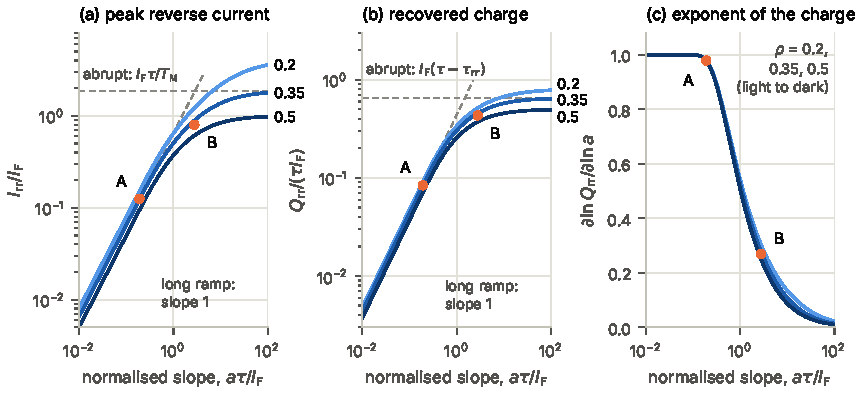
\includegraphics[width=\textwidth]{../lauritzen_ma_datasheet_conversion/figures/fig_map.pdf}
\caption{Recovery of the model against the normalised slope $a\tau/\IF = 1/\lambda$, for three values of $\rho$. (a) Peak reverse current and (b) recovered charge, with the two asymptotes of the middle curve: the long ramp \eqref{eq:long}, with slope one, and the abrupt commutation \eqref{eq:abrupt}, a constant. (c) Local exponent of the charge against the slope, \eqref{eq:exponents}. The points A and B are the two worked examples of Sec.~\ref{sec:examples} at their datasheet conditions.}
\label{fig:map}
\end{figure}

\subsection{Long ramp and abrupt commutation}
\label{sec:limitsramp}
\emph{Long ramp} ($\lambda \to \infty$). The exponential of \eqref{eq:peak} vanishes:
\begin{equation}
\Irr = a\,(\tau - \taurr) = \frac{a\,\tau^2}{\tau+\TM} , \qquad \ta = \tau - \taurr , \qquad \Qrr = \frac{a}{2}\,\bigl(\tau^2 - \taurr^2\bigr) .
\label{eq:long}
\end{equation}
Peak and charge are proportional to the slope and do not depend on the forward current. The time to the peak is a constant of the diode: it is the delay $\tau - \taurr$ of \eqref{eq:filter}.

The factor $1 - e^{-\xi}$ of \eqref{eq:peak}, with $\xi = \Tone/\tau$, says how long a ramp has to be. Table~\ref{tab:long} gives what is missing to the long-ramp values. A ramp is long, for the purpose of a conversion, when it lasts five lifetimes from the forward current to the peak; with three lifetimes the long-ramp formulas are off by \SI{\lmFDefThree}{\percent} on the peak and by up to \SI{\lmQDefHiThree}{\percent} on the charge.

\begin{table}[htb]
\centering\small
\caption{Peak current and charge of the model on a ramp of finite length, relative to the long-ramp values \eqref{eq:long}. The range of the charge is for $\rho$ from 0.5 to 0.1.}
\label{tab:long}
\begin{tabular}{@{}lcccc@{}}
\toprule
Length of the ramp, $\xi = \Tone/\tau$ & 2 & 3 & 4 & 5 \\
\midrule
$\Irr$: what is missing to the long-ramp value & \SI{\lmFDefTwo}{\percent} & \SI{\lmFDefThree}{\percent} & \SI{\lmFDefFour}{\percent} & \SI{\lmFDefFive}{\percent} \\
$\Qrr$: what is missing to the long-ramp value & \SIrange{\lmQDefLoTwo}{\lmQDefHiTwo}{\percent} & \SIrange{\lmQDefLoThree}{\lmQDefHiThree}{\percent} & \SIrange{\lmQDefLoFour}{\lmQDefHiFour}{\percent} & \SIrange{\lmQDefLoFive}{\lmQDefHiFive}{\percent} \\
\bottomrule
\end{tabular}
\end{table}

\emph{Abrupt commutation} ($\lambda \to 0$). The ramp is so fast that nothing recombines before the junction blocks. The middle charge is still $\tau\IF$ when the edge charge is pulled to zero, and \eqref{eq:blocked} gives
\begin{equation}
\Irr \to \IF\,\frac{\tau}{\TM} , \qquad \Qrr \to \IF\,(\tau - \taurr) = \IF\,\frac{\tau^2}{\tau+\TM} .
\label{eq:abrupt}
\end{equation}
Peak and charge are proportional to the forward current and no longer depend on the slope. These are the largest values the model can give for a forward current.

\subsection{Charge balance}
Of the charge present at the current zero, \eqref{eq:qzero}, only a part comes out of the terminals. The rest recombines during the recovery. On a long ramp, from \eqref{eq:long},
\begin{equation}
\frac{\Qrr}{\qM(t_0)} = \frac{1-\rho^2}{2} .
\label{eq:fraction}
\end{equation}
Less than half of the charge at the current zero is recovered: \SI{\lmQfracRhoLo}{\percent} for $\rho = 0.2$, \SI{\lmQfracRhoMid}{\percent} for $\rho = 0.35$, \SI{\lmQfracRhoHi}{\percent} for $\rho = 0.5$. In an abrupt commutation the recovered part of the static charge $\tau\IF$ is $1-\rho$, by \eqref{eq:abrupt}. The recovered charge of a datasheet is therefore never the stored charge of the diode, and the lifetime cannot be read as $\Qrr/\IF$ (Sec.~\ref{sec:others}).

\subsection{Dependence on the slope and on the forward current}
\label{sec:exponents}
While the junction conducts, the equations \eqref{eq:conducting} are linear, and the blocking condition $\qE = 0$ does not change if the current and the charges are all multiplied by the same factor. So if the slope and the forward current are both multiplied by $c$, the whole waveform is multiplied by $c$: $\Irr$ and $\Qrr$ are homogeneous functions of degree one of the pair $(a, \IF)$, as \eqref{eq:normdef} and \eqref{eq:norm} show. By Euler's theorem on homogeneous functions
\begin{equation}
\frac{\partial \ln \Irr}{\partial \ln a} + \frac{\partial \ln \Irr}{\partial \ln \IF} = 1 , \qquad
\frac{\partial \ln \Qrr}{\partial \ln a} + \frac{\partial \ln \Qrr}{\partial \ln \IF} = 1 .
\label{eq:euler}
\end{equation}
In a log-log plot the slope of a curve against $a$ and the slope of the curve against $\IF$ add up to one, at every point. The exponents against the slope follow from \eqref{eq:norm} (Appendix~\ref{app:exponents}):
\begin{equation}
\frac{\partial \ln \Irr}{\partial \ln a} = 1 - \frac{\lambda\,(1-\rho-y)}{y\,(\rho+y)} , \qquad
\frac{\partial \ln \Qrr}{\partial \ln a} = 1 - \frac{\lambda\,(1-\rho-y)}{y^2/2+\rho\,y} .
\label{eq:exponents}
\end{equation}
On a long ramp $y = 1-\rho$ and both exponents are one: the recovery is proportional to the slope and blind to the forward current. In an abrupt commutation both are zero and the recovery is proportional to the forward current. Figure~\ref{fig:map}c shows the passage from one to the other, which takes about two decades of slope around $a\tau = \IF$.

%=====================================================================
\section{From the model to the datasheet quantities}
\label{sec:direct}
\subsection{Recovery time and softness}
\label{sec:trr}
With the exponential tail \eqref{eq:tail}, every convention for the end of the recovery gives a fall time proportional to the tail time constant:
\begin{equation}
\tb = \kappa\,\taurr , \qquad \trr = \ta + \kappa\,\taurr .
\label{eq:trr}
\end{equation}
For a straight line through the points at the fractions $f_\mathrm{A}$ and $f_\mathrm{B}$ of the peak,
\begin{equation}
\kappa = \ln\frac{1}{f_\mathrm{A}} + \frac{f_\mathrm{A}}{f_\mathrm{A}-f_\mathrm{B}}\,\ln\frac{f_\mathrm{A}}{f_\mathrm{B}} ,
\label{eq:kappaline}
\end{equation}
and for the instant at which the current has fallen to the fraction $f$ of the peak, $\kappa = \ln(1/f)$. Table~\ref{tab:kappa} gives the values. Between the conventions the fall time of the same waveform differs by up to \num{\lmKSpread} tail time constants, so a recovery time cannot be converted without its convention.

\begin{table}[htb]
\centering\small
\caption{Conventions for the end of the recovery and fall time of an exponential tail, $\tb = \kappa\,\taurr$.}
\label{tab:kappa}
\begin{tabular}{@{}lcl@{}}
\toprule
Convention & $\kappa$ & Used in \\
\midrule
straight line through \SI{90}{\percent} and \SI{25}{\percent} of the peak, extended to zero & \lmKLine & \cite{iec60747}, 3.5.2 Note~5; \cite{an6481}, Sec.~2.1 \\
current fallen to \SI{25}{\percent} of the peak & \lmKQuarter & \cite{an5028} ($k$ usually \num{0.25}) \\
current fallen to \SI{10}{\percent} of the peak & \lmKTen & \cite{mathworks}, \cite{plecs} \\
triangle with the same charge as the tail & 2 & this document, \eqref{eq:soft} \\
\bottomrule
\end{tabular}
\end{table}

This document measures the softness with the ratio of the charge of the tail to the charge of the triangle,
\begin{equation}
s = \frac{\Irr\,\taurr}{\Irr\,\ta/2} = \frac{2\,\taurr}{\ta} .
\label{eq:soft}
\end{equation}
It is the ratio $\tb/\ta$ for the triangle of equal charge ($\kappa = 2$); the ratio $\tb/\ta$ of the straight-line convention is \num{\lmKLineHalf}\,$s$. From \eqref{eq:peak}, $\ta = (\tau-\taurr)\,(1-e^{-\xi})$, so
\begin{equation}
s = \frac{2\,\TM}{\tau}\,\frac{1}{1-e^{-\xi}} \quad\longrightarrow\quad s = \frac{2\,\TM}{\tau} \quad \text{on a long ramp.}
\label{eq:softlong}
\end{equation}
On a long ramp the softness of the model is a constant of the diode: twice the ratio of its two parameters. It does not depend on the slope, on the forward current or on the voltage. On a short ramp the softness is larger, because the triangle shrinks and the tail time constant does not. The documentation \cite{mathworks} uses the stretch factor $\trr\,a/\Irr$ with the \SI{10}{\percent} convention, which is $1 + (\ln 10/2)\,s$; its typical value of 3 corresponds to $s = \lmSofStretchThree$.

\subsection{Recovered charge}
Equation \eqref{eq:qrr} is the integral of the whole reverse current. If the integral ends where the current has fallen to the fraction $f$ of the peak, as in the standard with $f = \SI{\lmPEndPct}{\percent}$, the fraction $f$ of the tail charge is cut:
\begin{equation}
Q_\mathrm{r} = \frac{\Irr\,\ta}{2} + (1-f)\,\Irr\,\taurr .
\label{eq:qrp}
\end{equation}
The integral then lasts $\ln(1/f) = \lmTEndTaus$ tail time constants. The difference from \eqref{eq:qrr} is below the tolerance of any datasheet value; \eqref{eq:qrp} is used in Sec.~\ref{sec:cell} to compare a simulation with the closed form on equal terms. A second difference is the charge of the junction capacitance, which a measured value includes and \eqref{eq:qrr} does not (Sec.~\ref{sec:blocking}).

The estimate $\Qrr \approx \Irr\,\trr/2$ is exact with the equal-charge convention. With the straight-line convention it misses \SI{\lmKLineLossPct}{\percent} of the tail charge, and with the \SI{10}{\percent} convention it adds \SI{\lmKTenGainPct}{\percent} to it.

\subsection{The triangle formulas}
\label{sec:triangle}
Many textbooks and application notes describe the reverse current with two straight segments: the rise in $\ta$ with the slope $a$ and a linear fall in $\tb = S\,\ta$ [M]~\cite{mohan}. From the geometry,
\begin{equation}
\Qrr = \frac{\Irr\,\trr}{2} = \frac{\Irr^2}{2a}\,(1+S) , \qquad \Irr = \sqrt{\frac{2\,a\,\Qrr}{1+S}} , \qquad \trr = \sqrt{\frac{2\,\Qrr\,(1+S)}{a}} .
\label{eq:triangle}
\end{equation}
These are the relations of the model with the equal-charge convention: \eqref{eq:qrr} reads $\Qrr = (\Irr^2/2a)\,(1+s)$, so $S$ coincides with the softness $s$ of \eqref{eq:soft} and $\trr$ with the row $\kappa = 2$ of Table~\ref{tab:kappa}. With the straight line of the standard the same diode has $\tb/\ta = \num{\lmKLineHalf}\,s$.

Equations \eqref{eq:triangle} are identities between the quantities of one and the same waveform, not scaling laws. The second is often read as $\Irr \propto \sqrt{a}$, but it holds in this form only if $\Qrr$ and $S$ do not change with the slope. In the two-charge model, on a long ramp, $\Irr$ and $\Qrr$ both grow in proportion to $a$ (Sec.~\ref{sec:exponents}), and in an abrupt commutation they no longer depend on the slope, \eqref{eq:abrupt}. The square-root behaviour is the short-ramp limit of the one-charge model ($\TM = 0$, $S = 0$), in which $\Qrr$ tends to the static charge (Sec.~\ref{sec:ccsolutions}); with two charges it appears only as an intermediate regime, when $\TM \ll \tau$. For a measured curve $\Qrr \propto a^{m}$, at constant softness \eqref{eq:triangle} gives $\Irr \propto a^{(1+m)/2}$.
\subsection{Peak voltage and energy in an inductive commutation}
\label{sec:energy}
In the cell of Fig.~\ref{fig:commcell}a without snubber and without capacitance, the diode voltage stays near zero up to the peak of the reverse current. In the tail the diode imposes the current \eqref{eq:tail} on the inductance, and its reverse voltage is
\begin{equation}
v_\mathrm{R}(t) = \VR + \frac{\Ls\,\Irr}{\taurr}\,e^{-(t-\Tone)/\taurr} .
\end{equation}
The peak is at the blocking instant. With $\Ls = \VR/a$,
\begin{equation}
\Vrm = \VR + \frac{\Ls\,\Irr}{\taurr} = \VR\,\Bigl(1 + \frac{\ta}{\taurr}\Bigr) = \VR\,\Bigl(1 + \frac{2}{s}\Bigr) .
\label{eq:vrm}
\end{equation}
The peak voltage depends on the softness only: a diode with $s = 1$ triples the applied voltage, one with $s = 4$ adds half of it. The energy dissipated in the diode during the tail is
\begin{equation}
\Erec = \int v_\mathrm{R}\,|i|\,\diff t = \VR\,\Irr\,\taurr + \frac{\Ls\,\Irr^2}{2} = \VR\,\Qrr .
\label{eq:erec}
\end{equation}
The first form is in \cite{mathworks}; the second follows with $\Ls = \VR/a$ and \eqref{eq:qrr}. It contains the energy that the inductance holds at the peak.

Without capacitance the voltage steps from zero to $\Vrm$ at the blocking instant. A real circuit always has a capacitance $C$ across the diode, starting with the junction capacitance. Since the diffusion current of the blocked junction, \eqref{eq:blocked}, does not depend on the voltage, the diode remains the current source \eqref{eq:tail}, and the capacitance carries the difference between the current of the inductance and that of the diode. The reverse voltage then obeys
\begin{equation}
\Ls\,\frac{\diff}{\diff t}\Bigl(C\,\frac{\diff v_\mathrm{R}}{\diff t}\Bigr) + v_\mathrm{R} = \VR + \frac{2\,\VR}{s}\;e^{-(t-\Tone)/\taurr} , \qquad v_\mathrm{R}(\Tone) = 0 , \qquad \frac{\diff v_\mathrm{R}}{\diff t}(\Tone) = 0 :
\label{eq:vlc}
\end{equation}
the voltage starts from zero, and at the blocking instant the current of the inductance is still that of the diode. The right-hand side is the voltage that the diode would have without capacitance, and \eqref{eq:vrm} is its initial value: the capacitance turns the step into an oscillation around that voltage. With a constant capacitance and without damping the first maximum $\hat v_\mathrm{R}$ lies between $2\VR$ and $2\Vrm$. If the oscillation is fast against the tail, $\sqrt{\Ls C} \ll \taurr$, the right-hand side is still $\Vrm$ when the voltage reaches its maximum, and $\hat v_\mathrm{R} \to 2\Vrm$. If it is slow, $\sqrt{\Ls C} \gg \taurr$, the tail dies out before the voltage rises, and the current $\Irr$ of the inductance passes to the capacitance:
\begin{equation}
\hat v_\mathrm{R} \to \VR\left[1 + \sqrt{1 + \frac{\ta^2}{\Ls\,C}}\,\right] ,
\label{eq:vpkslow}
\end{equation}
which falls to $2\VR$ only for $\sqrt{\Ls C} \gg \ta$. A lossless capacitance therefore never brings the peak below $2\VR$, and a small capacitance doubles it compared with \eqref{eq:vrm}.

The junction capacitance does more, because it decreases as the voltage grows, \eqref{eq:cj}. If its oscillation is fast against the tail, the right-hand side of \eqref{eq:vlc} is the constant $\Vrm$; multiplying the equation by the current of the capacitance and integrating, the first maximum, where that current returns to zero, satisfies $\int_0^{\hat v_\mathrm{R}} \mbox{$(\Vrm - v_\mathrm{R})$}\,\Cj\,\diff v_\mathrm{R} = 0$. With $m_\mathrm{j} = 1/2$ and no other capacitance,
\begin{equation}
\hat v_\mathrm{R} = 3\,\Vrm - \frac{\Vbi}{2}\left(\sqrt{9 + \frac{12\,\Vrm}{\Vbi}} - 3\right) \approx 3\,\Vrm - \sqrt{3\,\Vbi\,\Vrm} ,
\label{eq:vpkcj}
\end{equation}
almost three times the peak without capacitance. To bring the peak back towards $\Vrm$, or below it, damping is needed in practice, that is the resistor of a snubber (Sec.~\ref{sec:cell}): without losses only a large capacitance can do it, and only if $s < 2$, that is if $\Vrm > 2\VR$ (for $s = 1$ it takes $\sqrt{\Ls C} > \num{1.3}\,\taurr$), and the oscillation around $\VR$ is not damped. With a capacitance, moreover, the terminal current keeps growing in magnitude as long as $v_\mathrm{R} < \VR$: its peak is higher than that of the diffusion current, and delayed with respect to it.

With an RC snubber across the diode the balance of the energy from the current zero to the end of the transient is
\begin{equation}
E_\mathrm{D} + E_\mathrm{R} = \VR\,\Qrr + \frac{\Csn\,\VR^2}{2} ,
\label{eq:ebal}
\end{equation}
where $E_\mathrm{D}$ is the energy dissipated in the diode and $E_\mathrm{R}$ the energy dissipated in the snubber resistor. The source delivers the energy $\VR\,(\Qrr + \Csn\VR)$, that is, $\VR$ times the charge of the diode plus that of the snubber capacitor, and the capacitor keeps $\Csn\VR^2/2$ of it. The sum does not depend on the snubber resistor: the snubber moves a part of $\VR\,\Qrr$ from the diode to the resistor and adds the loss due to the charging of its capacitor, $\Csn\VR^2/2$.

\subsection{In a switching leg}
\label{sec:switchingleg}
Equations \eqref{eq:vrm} and \eqref{eq:erec} hold for the cell of Fig.~\ref{fig:commcell}a, where the same inductance sets the slope and is subjected to the tail. In a switching leg (Fig.~\ref{fig:commcell}b) the slope is imposed by the switch, and the drop $\Ls a$ on the stray inductance is only a part of $\Vdc$. With the same idealisation, that is with the junction blocking at the peak and the switch already in full conduction during the tail, the reverse voltage of the diode is $\Vdc + (\Ls\Irr/\taurr)\,e^{-(t-\Tone)/\taurr}$. With $\Irr/\taurr = 2a/s$,
\begin{equation}
\Vrm = \Vdc + \frac{2\,\Ls\,a}{s} , \qquad
\Erec = \Vdc\,\Irr\,\taurr + \frac{\Ls\,\Irr^2}{2} = \Vdc\,\Qrr\;\frac{s + \Ls a/\Vdc}{1+s} .
\label{eq:vrmleg}
\end{equation}
For $\Ls a = \Vdc$ one finds \eqref{eq:vrm} and \eqref{eq:erec} again. For $\Ls a \ll \Vdc$, the normal case, the overvoltage is small and the energy in the diode is
\begin{equation}
\Erec \approx \Vdc\,\Qrr\,\frac{s}{1+s} :
\label{eq:erecleg}
\end{equation}
the diode dissipates at full voltage the charge of the tail alone. The factor $s/(1+s)$ is \num{0.5} for $s = 1$ and \num{0.8} for $s = 4$: it is the form factor $k_\mathrm{E}$, between \num{0.5} and \num{0.8}, with which $\Erec \approx k_\mathrm{E}\,\Vdc\,\Qrr$ is usually estimated. Equations \eqref{eq:vrmleg} and \eqref{eq:erecleg} are written for a switch already in full conduction: a real switch still sustains a part of the voltage during the tail, and the voltage and the energy of the diode are lower. As in the cell, the capacitances across the diode then add an oscillation (Sec.~\ref{sec:energy}), but the factors 2 and 3 of that section hold for a voltage applied as a step and do not carry over to $\Vdc$: in a real switching leg the voltage of the diode rises while that of the switch falls, at a rate set by the drive. A voltage ramp of duration $t_\mathrm{v}$ excites in a lossless $\Ls C$ circuit with a constant $C$ an oscillation whose amplitude is not larger than $2\sqrt{\Ls C}/t_\mathrm{v}$ times the excursion of the ramp, hence small against $\Vdc$ if the rise lasts several periods $2\pi\sqrt{\Ls C}$ (this limit does not hold for the junction capacitance alone, which decreases as the voltage rises). The inductive part $\Ls a\,(1+2/s)$, however, is still applied as a step at the blocking instant, as in the cell with $\VR = \Ls a$: the oscillation it excites has, with a constant $C$ and no losses, an amplitude between $\Ls a$ and $\Ls a\,(1+2/s)$, whatever the rate at which the voltage rises.

The rest of the energy that the source delivers for the recovery, $\Vdc\,\Irr\,\ta/2$, is dissipated in the switch. During $\ta$ the diode is still a short circuit, and the switch conducts the current of the load plus the reverse current with the whole voltage across it. Compared with a diode without recovery, its turn-on energy grows by
\begin{equation}
\Delta E_\mathrm{on} \approx \Vdc\,\Bigl(I_\mathrm{L} + \frac{\Irr}{2}\Bigr)\,\ta ,
\label{eq:eon}
\end{equation}
in which the first term, usually the larger, is the current of the load that the switch carries at full voltage for the extra time $\ta$. The recovery of the diode weighs on the switch more than on the diode; Section~\ref{sec:losses} gives a numerical example of it.
\subsection{Other test circuits}
\label{sec:othertests}
\emph{Resistive commutation.} Small and fast diodes are often tested with a step: the forward current $\IF$ is reversed abruptly and the circuit limits the reverse current to $\IR$. While the junction conducts, the reverse current stays at $\IR$; this is the storage phase. Equation \eqref{eq:conducting} with $i = -\IR$ gives $\qM(t) = -\tau\IR + \tau\,(\IF+\IR)\,e^{-t/\tau}$, and $\qE = \qM - \TM\IR$ reaches zero at the storage time
\begin{equation}
\ts = \tau\,\ln\!\left[\Bigl(1+\frac{\IF}{\IR}\Bigr)\,\frac{\tau}{\tau+\TM}\right] \qquad \text{if} \quad \frac{\IF}{\IR} > \frac{\TM}{\tau} .
\label{eq:ts}
\end{equation}
After the storage time the current decays from $\IR$ with the time constant $\taurr$. If $\IF/\IR \leq \TM/\tau$ there is no storage phase: the junction blocks at once, the reverse current starts from $\IF\,\tau/\TM$, which is the abrupt limit \eqref{eq:abrupt}, and decays from there. With $\TM \to 0$ \eqref{eq:ts} becomes \eqref{eq:storage}, the storage time of the one-charge model; with a finite transit time the storage time is shorter than that of \eqref{eq:storage} by $\tau\ln(1+\TM/\tau)$, and a $\tau$ read with \eqref{eq:storage} is underestimated. The absence of the storage phase for $\IF/\IR \leq \TM/\tau$ is a property of the two-charge model: in a distributed base the edge always takes a finite time to empty, and for a base that is wide against the diffusion length the storage time is given by $\operatorname{erf}\sqrt{\ts/\tau} = 1/(1+\IR/\IF)$ [M]~\cite{sze}.

\emph{Half-sine pulse.} The standard has a half-sinusoidal and a rectangular measuring method (\cite{iec60747}, 6.3.5). For a sinusoidal current $\hat I\sin\omega t$ that has lasted long on the scale of $\tau$, \eqref{eq:filter} gives the edge charge as a sinusoid delayed by the phase $\arctan\omega\tau - \arctan\omega\taurr$. The junction blocks at this phase after the current zero, so
\begin{equation}
\Irr = \hat I\,\sin\bigl(\arctan\omega\tau - \arctan\omega\taurr\bigr) .
\label{eq:sine}
\end{equation}
For $\omega\tau \ll 1$ this is $\omega\hat I\,(\tau-\taurr)$: the long-ramp result \eqref{eq:long} with the slope $a = \omega\hat I$ of the sinusoid at its zero.

%=====================================================================
\part{From the datasheet to the model}

\section{Conversion of the recovery data}
\label{sec:inverse}
\subsection{From the peak current and the charge}
\label{sec:invpq}
The datasheet gives $\Irr$ and $\Qrr$ at a slope $a$ and a forward current $\IF$. The conversion has four steps.
\begin{enumerate}
\item Time to the peak: $\ta = \Irr/a$.
\item Tail time constant, from \eqref{eq:qrr}:
\begin{equation}
\taurr = \frac{\Qrr}{\Irr} - \frac{\Irr}{2a} .
\label{eq:taurr}
\end{equation}
This step is exact for any ramp; the same relation is Eq.~(2) of \cite{an6481}. It needs $\Qrr > \Irr^2/(2a)$: the charge has to be larger than the triangle. A pair of data that violates the condition has no tail and cannot be represented by the model.
\item Lifetime, from \eqref{eq:peak} written as
\begin{equation}
\tau = \taurr + \frac{\ta}{1 - e^{-\Tone/\tau}} , \qquad \Tone = \frac{\IF+\Irr}{a} .
\label{eq:iter}
\end{equation}
Equation \eqref{eq:iter} is used as an iteration: the right-hand side is evaluated with the current value of $\tau$, starting from $\tau = \taurr + \ta$. The iteration converges for any data, to the only solution, and at each step the error shrinks by a factor smaller than $\Irr/(\IF+\Irr)$ (Appendix~\ref{app:contraction}).
\item Transit time, from the definition of $\taurr$:
\begin{equation}
\TM = \frac{\tau\,\taurr}{\tau - \taurr} .
\label{eq:tm}
\end{equation}
\end{enumerate}
On a long ramp the exponential of \eqref{eq:iter} is zero and the starting value is already the result:
\begin{equation}
\tau = \taurr + \ta = \frac{\Qrr}{\Irr} + \frac{\Irr}{2a} , \qquad \TM = \frac{\tau\,\taurr}{\ta} .
\label{eq:longinv}
\end{equation}
This is the closed form usually found in the literature on the model; it does not contain the forward current.

\subsection{When the closed form is enough}
\label{sec:valid}
The closed form \eqref{eq:longinv} is exact for $\xi = \Tone/\tau \to \infty$. Whether a datasheet point is on a long ramp can be seen from the data alone, because $\xi$ follows from the ratio $\Irr/\IF$ and from the softness $s = 2\taurr/\ta$:
\begin{equation}
\xi = \frac{1 + \IF/\Irr}{s/2 + 1/(1-e^{-\xi})} \;\approx\; \frac{1 + \IF/\Irr}{1 + s/2} .
\label{eq:xdata}
\end{equation}
A set obtained with the closed form from a point that is not on a long ramp is not the diode of the datasheet: put back on the test ramp it returns a lower peak and a lower charge. Figure~\ref{fig:inversion} shows this error and Table~\ref{tab:valid} gives the limits. When the peak reverse current of the datasheet is below a tenth of the forward current, the set of the closed form returns the peak and the charge within \SI{\lmTenthErrTwo}{\percent} for a softness up to 2 and within \SI{\lmTenthErrFour}{\percent} for a softness of 4. For a fast diode tested with a peak reverse current close to the forward current it is wrong by tens of percent, and \eqref{eq:iter} has to be used. The iteration costs nothing, so the simple rule is to iterate always.

\begin{table}[htb]
\centering\small
\caption{Largest ratio $\Irr/\IF$ of the datasheet point for which the set of the closed form \eqref{eq:longinv} returns the peak current of the datasheet within the stated error.}
\label{tab:valid}
\begin{tabular}{@{}lcccc@{}}
\toprule
Softness of the datasheet point, $s = 2\taurr/\ta$ & 0.5 & 1 & 2 & 4 \\
\midrule
$\Irr$ returned within \SI{1}{\percent} for $\Irr/\IF$ below & \lmRatioOneHalf & \lmRatioOneOne & \lmRatioOneTwo & \lmRatioOneFour \\
$\Irr$ returned within \SI{5}{\percent} for $\Irr/\IF$ below & \lmRatioFiveHalf & \lmRatioFiveOne & \lmRatioFiveTwo & \lmRatioFiveFour \\
\bottomrule
\end{tabular}
\end{table}

\begin{figure}[htb]
\centering
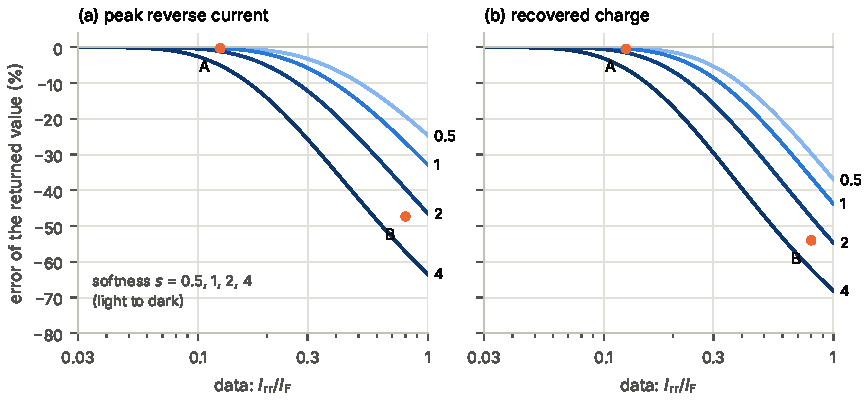
\includegraphics[width=\textwidth]{../lauritzen_ma_datasheet_conversion/figures/fig_inversion.pdf}
\caption{Error of the long-ramp closed form \eqref{eq:longinv}: the set it gives is put back on the test ramp and (a) its peak current and (b) its charge are compared with the data, against the ratio $\Irr/\IF$ of the datasheet point and for four values of the softness. A and B are the two worked examples.}
\label{fig:inversion}
\end{figure}

\subsection{From other pairs of data}
\label{sec:pairs}
The recovery has two parameters, so two independent data at one test condition are needed. With pairs other than $(\Irr, \Qrr)$ the first two steps of Sec.~\ref{sec:invpq} change and the other two stay.

\emph{Peak current and recovery time.} From \eqref{eq:trr}, with the $\kappa$ of the convention of the datasheet,
\begin{equation}
\taurr = \frac{\trr - \Irr/a}{\kappa} .
\label{eq:fromtrr}
\end{equation}
It needs $\trr > \Irr/a$.

\emph{Charge and recovery time.} Eliminating $\taurr$ between \eqref{eq:qrr} and \eqref{eq:trr} gives a quadratic equation for the peak current, $(1-\kappa/2)\,\Irr^2 - a\,\trr\,\Irr + \kappa\,a\,\Qrr = 0$, with the solution
\begin{equation}
\Irr = \frac{a}{2-\kappa}\left[\trr - \sqrt{\trr^2 - \frac{2\,\kappa\,(2-\kappa)\,\Qrr}{a}}\,\right] \quad (\kappa \neq 2) , \qquad \Irr = \frac{2\,\Qrr}{\trr} \quad (\kappa = 2) .
\label{eq:fromqt}
\end{equation}
This is the root with $0 < \Irr < a\,\trr$, that is, with $\taurr > 0$. For $\kappa \geq 1$, as in all the conventions of Table~\ref{tab:kappa}, it exists and is unique if and only if $\Qrr < a\,\trr^2/2$, that is, if the charge is smaller than that of the triangle that the ramp would describe in the whole recovery time. Then \eqref{eq:fromtrr} gives $\taurr$.

\emph{One datum only.} With the charge alone, or the recovery time alone, the shape has to be assumed. With an assumed softness $s$, from \eqref{eq:qrr} and \eqref{eq:soft},
\begin{equation}
\Irr = \sqrt{\frac{2\,a\,\Qrr}{1+s}} , \qquad \taurr = \frac{s\,\Irr}{2a} .
\label{eq:fromq}
\end{equation}

\emph{Three data.} When the datasheet gives $\Irr$, $\Qrr$ and $\trr$, the three are consistent with an exponential tail if $\Qrr = \Irr\,[\ta/2 + (\trr-\ta)/\kappa]$. Usually they are not exactly, because a real tail is not an exponential. The pair $(\Irr, \Qrr)$ is then the better choice: the peak and the charge are what the circuit feels, and they do not depend on a convention. The recovery time is a check.

\subsection{Sensitivity to the data}
\label{sec:sens}
Datasheet values have tolerances, and the two values of a pair are often maxima that do not belong to the same device. On a long ramp the logarithmic derivatives of \eqref{eq:taurr} and \eqref{eq:longinv} are
\begin{equation}
\begin{aligned}
\frac{\diff\taurr}{\taurr} &= \frac{1+s}{s}\,\frac{\diff\Qrr}{\Qrr} - \frac{2+s}{s}\,\frac{\diff\Irr}{\Irr} + \frac{1}{s}\,\frac{\diff a}{a} , \\
\frac{\diff\tau}{\tau} &= \frac{1+s}{2+s}\,\frac{\diff\Qrr}{\Qrr} - \frac{s}{2+s}\,\frac{\diff\Irr}{\Irr} - \frac{1}{2+s}\,\frac{\diff a}{a} , \\
\frac{\diff\TM}{\TM} &= \frac{\diff\tau}{\tau} + \frac{\diff\taurr}{\taurr} - \frac{\diff\Irr}{\Irr} + \frac{\diff a}{a} .
\end{aligned}
\label{eq:sens}
\end{equation}

\begin{table}[htb]
\centering\small
\caption{Relative change of the parameters for a relative change of one datum of one percent, on a long ramp, from \eqref{eq:sens}.}
\label{tab:sens}
\begin{tabular}{@{}lccccccccc@{}}
\toprule
 & \multicolumn{3}{c}{$s = 0.5$} & \multicolumn{3}{c}{$s = 1$} & \multicolumn{3}{c}{$s = 2$} \\
\cmidrule(lr){2-4}\cmidrule(lr){5-7}\cmidrule(l){8-10}
Datum & $\tau$ & $\taurr$ & $\TM$ & $\tau$ & $\taurr$ & $\TM$ & $\tau$ & $\taurr$ & $\TM$ \\
\midrule
$\Qrr$ & $+\lmSensTauQHalf$ & $+\lmSensTrrQHalf$ & $+\lmSensTmQHalf$ & $+\lmSensTauQOne$ & $+\lmSensTrrQOne$ & $+\lmSensTmQOne$ & $+\lmSensTauQTwo$ & $+\lmSensTrrQTwo$ & $+\lmSensTmQTwo$ \\
$\Irr$ & $-\lmSensTauIHalf$ & $-\lmSensTrrIHalf$ & $-\lmSensTmIHalf$ & $-\lmSensTauIOne$ & $-\lmSensTrrIOne$ & $-\lmSensTmIOne$ & $-\lmSensTauITwo$ & $-\lmSensTrrITwo$ & $-\lmSensTmITwo$ \\
$a$ & $-\lmSensTauAHalf$ & $+\lmSensTrrAHalf$ & $+\lmSensTmAHalf$ & $-\lmSensTauAOne$ & $+\lmSensTrrAOne$ & $+\lmSensTmAOne$ & $-\lmSensTauATwo$ & $+\lmSensTrrATwo$ & $+\lmSensTmATwo$ \\
\bottomrule
\end{tabular}
\end{table}

Table~\ref{tab:sens} reads as follows. The lifetime is a robust result: all its coefficients are below one. The tail time constant and the transit time are fragile, the more so the snappier the diode: $\taurr$ is the difference of two terms of similar size, $\Qrr/\Irr$ and $\ta/2$, and for $s = 0.5$ a peak current higher by \SI{1}{\percent} lowers $\TM$ by \SI{\lmSensTmIHalf}{\percent}. The softness of the model, $2\TM/\tau$, is therefore known only roughly from a pair of datasheet values. When the peak voltage or the damping of a commutation depend on it, the transit time has to be checked on a measured waveform, or the calculation repeated with $\TM$ at the two ends of its range.

\subsection{Which data to convert}
\label{sec:which}
\begin{itemize}
\item \emph{Maximum or typical.} A set converted from the maximum $\Qrr$ and $\Irr$ is the device with the largest charge. For the spread between the devices of a series connection a second device with a lower charge is needed. If only its charge is known, the softness is kept: on a long ramp \eqref{eq:long} gives $\Qrr \propto \tau^2$ and $\Irr \propto \tau$ at a fixed ratio $\TM/\tau$, so a device with the charge $\Qrr'$ at the same slope has
\begin{equation}
\tau' = \tau\,\sqrt{\Qrr'/\Qrr} , \qquad \TM' = \TM\,\sqrt{\Qrr'/\Qrr} .
\label{eq:scale}
\end{equation}
\item \emph{Temperature.} A set holds at the temperature of its data. Lifetime and recovered charge grow with the temperature [M]~\cite{lutz}, so the data of the highest working temperature give the largest recovery. Between \SI{25}{\celsius} and \SI{125}{\celsius} the recovered charge of a fast diode typically grows by a factor of about two [M]~\cite{lutz}; at unchanged softness and slope the peak reverse current then grows by a factor of about $\sqrt{2}$, \eqref{eq:triangle}. If the datasheet gives the charge at a second temperature only as a ratio or a curve, \eqref{eq:scale} applies if the test ramp is long; otherwise the new charge is converted with the softness of the first point, \eqref{eq:fromq}.
\item \emph{Test point.} If the datasheet gives the recovery at several slopes, the point to convert is the one nearest to the slope of the application. Section~\ref{sec:slope} explains why.
\end{itemize}

%=====================================================================
\section{Conduction and blocking parameters}
\label{sec:static}
\subsection{Forward characteristic}
\label{sec:forward}
From \eqref{eq:static} and \eqref{eq:terminal} the static characteristic of the model is
\begin{equation}
v = \Nem\,\VT\,\ln\Bigl(1 + \frac{i}{\IS}\Bigr) + \RS\, i .
\label{eq:vf}
\end{equation}
It has three parameters. The straight line \eqref{eq:line} has two numbers, so one parameter has to be chosen, and it is the emission coefficient $\Nem$. The line gives no information on it: a fit of \eqref{eq:vf} to three points of a straight line returns $\Nem = 0$.

\emph{Choice of $\Nem$.} At its working currents a power diode has the base in high injection. The carrier concentration at the edges of the base then grows with $e^{\vj/(2\VT)}$, where $\vj$ is, apart from the constant drop $\VM$, the sum of the voltages of the two junctions (Sec.~\ref{sec:vf}), and since $\qE$ stands for that concentration the model wants $\Nem = 2$. The value $\Nem = 1$ belongs to low injection, and the recombination in the emitters brings the slope of the junction part to intermediate values; at the terminals, where $\VM$ rises in the meantime, the slope can exceed $2\VT$ (Sec.~\ref{sec:emitter}). A fit to a measured curve can return still other values, because the three parameters then also absorb what the model does not have, for example a resistance of the base that depends on the current.

\emph{Tangent fit.} The model is made tangent to the line at one current $I_0$, for example the forward current of the application:
\begin{equation}
\RS = \rT - \frac{\Nem\,\VT}{I_0} , \qquad \IS = \frac{I_0}{e^{(\VTo + \Nem\VT)/(\Nem\VT)} - 1} .
\label{eq:tangent}
\end{equation}
The first relation matches the slopes, because the junction has the incremental resistance $\Nem\VT/I_0$; the second matches the voltages, because the junction voltage at $I_0$ is then $\VTo + \Nem\VT$. Everywhere else the model lies below the line, by $\Nem\VT\,(u - 1 - \ln u)$ with $u = i/I_0$.

\emph{Secant fit.} The model crosses the line at the two currents $I_1$ and $I_2$ at which the line crosses the real characteristic:
\begin{equation}
\RS = \rT - \frac{\Nem\,\VT\,\ln(I_2/I_1)}{I_2 - I_1} , \qquad \IS = \frac{I_1}{e^{[\VTo + (\rT-\RS)\,I_1]/(\Nem\VT)} - 1} .
\label{eq:secant}
\end{equation}
The first relation neglects $\IS$ against $I_1$. Both fits need $\RS \geq 0$, which limits the emission coefficient to $\Nem \leq \rT I_0/\VT$ for the tangent and to $\Nem \leq \rT\,(I_2-I_1)/(\VT\ln(I_2/I_1))$ for the secant.

\emph{Points of a curve.} For $i \gg \IS$ equation \eqref{eq:vf} is linear in the three unknowns $\Nem\VT$, $\Nem\VT\ln\IS$ and $\RS$:
\begin{equation}
v_k = \Nem\VT\,\ln i_k - \Nem\VT\,\ln\IS + \RS\, i_k .
\label{eq:points}
\end{equation}
Three points of the forward curve give the three parameters by a linear system, and more points by least squares. The points should span the working range of the current.

\emph{Implementations with $\tau\,\IS^{*}$.} A saturation current found from the static characteristic is the $\IS$ of \eqref{eq:qe}. An implementation that writes the junction law with $\tau\,\IS^{*}$ needs $\IS^{*} = \IS\,(\tau+\TM)/\tau$, \eqref{eq:isstar}. If the factor is forgotten the forward voltage of the model is too high by $\Nem\VT\ln[(\tau+\TM)/\tau]$, a few tens of millivolts.

\subsection{Blocking state and junction capacitance}
\label{sec:blocking}
\emph{Leakage.} The resistance $\Rr$ carries the reverse current of the blocking diode: $\Rr = V/I$ at the reverse voltage and at the temperature of interest. With the datasheet maximum, $\Rr = \Vrrm/\Irrm$. A resistance is the simplest element that does it and it is right at one voltage; the reverse current of a real diode depends little on the voltage and much on the temperature [M]~\cite{lutz}. During the recovery the leakage is of no account.

\emph{Junction capacitance.} The capacitance follows the convention of SPICE,
\begin{equation}
\Cj(\vj) = \frac{\Cjo}{(1 - \vj/\Vbi)^{m_\mathrm{j}}} \qquad \text{for } \vj < F_\mathrm{C}\,\Vbi ,
\label{eq:cj}
\end{equation}
continued by its tangent above $F_\mathrm{C} \Vbi$, with $\Vbi \approx \SI{0.7}{\volt}$, $m_\mathrm{j} = 0.5$ for an abrupt junction and $F_\mathrm{C} = 0.5$. If the datasheet gives the capacitance $C$ at a reverse voltage $V$, then $\Cjo = C\,(1+V/\Vbi)^{m_\mathrm{j}}$. If it does not, as happens for large rectifier diodes, $\Cjo$ is estimated with \eqref{eq:wsc}, which gives \SI{\pdScCjZero}{\nano\farad\per\centi\metre\squared} for $\ND = \SI{1e14}{\centi\metre^{-3}}$: the doping is that of the voltage class (Table~\ref{tab:blocking}), and the active area follows from the rated current with a density of the order of \SI{100}{\ampere\per\centi\metre\squared}. The estimate need not be accurate: the charge \eqref{eq:qc} is a small part of $\Qrr$, and the peak \eqref{eq:vpkcj} does not contain $\Cjo$. The law with $m_\mathrm{j} = 0.5$ holds as long as the space charge region widens into the base: in a punch-through base, beyond the voltage at which the space charge region reaches the buffer, the capacitance stays almost constant. The charge that brings the junction from zero to the reverse voltage $\VR$ is
\begin{equation}
Q_\mathrm{c} = \frac{\Cjo\,\Vbi}{1-m_\mathrm{j}}\left[\Bigl(1+\frac{\VR}{\Vbi}\Bigr)^{1-m_\mathrm{j}} - 1\right] .
\label{eq:qc}
\end{equation}
This charge flows in the reverse direction while the voltage builds up, and a measured recovered charge includes it (Sec.~\ref{sec:rrdata}). For a power diode it is small against the stored charge, \SI{\lmAQcPct}{\percent} and \SI{\lmBQcPct}{\percent} of $\Qrr$ in the two examples, so the conversion of Sec.~\ref{sec:inverse} can ignore it; where it is not small, $Q_\mathrm{c}$ is subtracted from the datasheet charge before the conversion. The capacitance has a second effect: it carries current while the voltage rises, so the peak of the current at the terminals is a little higher than the peak of the diffusion current, and delayed with respect to it (Sec.~\ref{sec:cell}). The capacitance then rings with the inductance of the circuit, already during the tail: without damping it raises the peak reverse voltage (Sec.~\ref{sec:energy}).

%=====================================================================
\section{What the model cannot reproduce}
\label{sec:limits}
The conversion gives a set that returns the datasheet point exactly. Away from that point the model follows its own laws, and they are not those of a real diode.

\subsection{Slope}
\label{sec:slope}
On a long ramp the model has $\Qrr \propto a$ and $\Irr \propto a$, \eqref{eq:long}. The curves of the datasheets of rectifier diodes and thyristors are much flatter: in a log-log plot of the charge against the slope they are close to straight lines with a slope well below one (for example \cite{an5950}, Figs.~12 and~13). The assumed diode A has such a curve with the exponent \num{\lmAQexp}. Figure~\ref{fig:curves} and Table~\ref{tab:awaya} show what follows: the set converted at \SI{\lmASlope}{\ampere\per\micro\second} gives at \SI{\lmAAwayALo}{\ampere\per\micro\second} a charge of \SI{\lmAAwayQrrALo}{\micro\coulomb} against \SI{\lmAAwayDsALo}{\micro\coulomb} of the curve, and at \SI{\lmAAwayAHi}{\ampere\per\micro\second} a charge \num{\lmAAwayRatioAHi} times that of the curve.

The reason is that the lifetime of a real diode is not a constant. Recombination gets faster when the carrier concentration rises, in particular through the recombination in the emitters (Sec.~\ref{sec:emitter}) \cite{schlangenotto1969}, so a fast ramp, which leaves more charge in the base, meets a shorter effective lifetime. A model with a constant $\tau$ cannot follow. The extended model of the same authors \cite{ma1993} adds the recombination in the emitters, at the cost of more parameters.

Seen from the model, each slope has its own parameter set. If a curve $\Qrr \propto a^{m}$ is converted point by point on a long ramp with the same softness, \eqref{eq:long} gives
\begin{equation}
\tau(a) = \tau(a_0)\,\Bigl(\frac{a}{a_0}\Bigr)^{-(1-m)/2} ,
\label{eq:taucurve}
\end{equation}
and the same law for $\TM$. With $m = \lmAQexp$ the lifetime falls as $a^{-\lmATauExpCurve}$: it doubles when the slope falls by a factor of seven. The rules that follow are:
\begin{itemize}
\item convert the datasheet point at the slope nearest to the slope of the application;
\item if the datasheet gives a curve, read the charge (and the peak current, if its curve is given) at the slope of the application and convert that point; if only the charge is read, keep the softness of the datasheet point and use \eqref{eq:fromq};
\item below the range of the curve, as in a line-commutated converter with a slope of a fraction of an ampere per microsecond, neither the model with a fixed set nor the extrapolated curve is right. The note in \texttt{research/diode-stack}, Sec.~6, treats this case with a recombination term that is quadratic in the charge, and gives a floor and a ceiling of the charge.
\end{itemize}
A parameter set is a local description of the diode: it is good near the slope at which it was converted. Its $\tau$ is the effective lifetime of that test point, not a property of the material.

\subsection{Forward current}
On a long ramp the recovery of the model does not depend on the forward current at all; on a short ramp it grows with it, and the exponents against the slope and against the forward current add up to one, \eqref{eq:euler}. This is a test that can be made on a datasheet before any conversion: if its curves against the slope and against the forward current have exponents that do not add up to one near the working point, no parameter set reproduces both. The set then has to be converted at the forward current of the application as well.

\subsection{Reverse voltage, temperature, forward recovery, tail}
\label{sec:otherlimits}
\begin{itemize}
\item \emph{Reverse voltage.} The tail \eqref{eq:tail} does not depend on the voltage across the diode, as the authors note for their own implementation \cite{pemodels}. A set converted at the reverse voltage of the datasheet test is used unchanged at another voltage. In a real diode the peak current and the charge depend on the voltage a little, and the softness can depend on it much more [M]~\cite{lutz}.
\item \emph{Temperature.} The equations contain the temperature only in $\VT$. The recovery parameters are valid at the temperature of the data (Sec.~\ref{sec:which}).
\item \emph{Forward recovery.} The model has a constant series resistance: it has no voltage overshoot at turn-on. The extended model \cite{ma1993} adds the conductivity modulation of the base.
\item \emph{Shape of the tail.} The tail of the model is always one exponential. A real tail can have two slopes or end abruptly, and then the triple $\Irr$, $\Qrr$, $\trr$ of the datasheet is not consistent with \eqref{eq:trr}.
\end{itemize}

%=====================================================================
\section{Other parameter sets and simulators}
\label{sec:others}
Table~\ref{tab:others} relates the parameters $\tau$ and $\TM$ of the two-charge model to those of other implementations and of two other diode models.

\begin{table}[htb]
\centering\small
\caption{The recovery parameters in other implementations and models.}
\label{tab:others}
\begin{tabular}{@{}>{\raggedright\arraybackslash}p{4.6cm}>{\raggedright\arraybackslash}p{4.2cm}>{\raggedright\arraybackslash}p{7.2cm}@{}}
\toprule
Model or implementation & Recovery parameters & Relation to $\tau$ and $\TM$ \\
\midrule
Library component \texttt{diode\_rr} (pwr-control library) & \texttt{tau}, \texttt{TM} & the same; junction law with $\tau\,\IS^{*}$, so $\IS^{*} = \IS(\tau+\TM)/\tau$, \eqref{eq:isstar} \\
\addlinespace
Diode block with charge dynamics \cite{mathworks} & carrier lifetime and transit time, or $\Irr$ and $a$ with one of $\trr$, stretch factor, $\Qrr$ & transit time $= \TM$; $\trr$ with the \SI{10}{\percent} convention; the documentation gives the ramp solution of Sec.~\ref{sec:ramp} and states that the peak condition is solved iteratively \\
\addlinespace
SPICE form on the web pages of the authors of the model \cite{pemodels} & \texttt{Tau}, \texttt{TT} & $\texttt{Tau} = \tau$, $\texttt{TT} = \TM$; ``approximate conversions'' $\Qrr = \texttt{Tau}\cdot\IF$ and $1/\trr = 1/\texttt{Tau} + 1/\texttt{TT}$ \\
\addlinespace
Diode of SPICE & \texttt{TT} & one charge, equal to $\texttt{TT}$ times the static current: $\tau = \texttt{TT}$ and $\TM = 0$, so $s = 0$ \\
\addlinespace
Behavioural diode with reverse recovery \cite{plecs} & two of $\trr$, $\Irr$, $\Qrr$, with the forward current and the slope of the test & not a charge model: the datasheet values are entered as they are; $\trr$ with the \SI{10}{\percent} convention \\
\bottomrule
\end{tabular}
\end{table}

\emph{The approximate conversions.} The two relations quoted in the third row are the abrupt-commutation limit of Sec.~\ref{sec:limitsramp}. With $\taurr \ll \tau$, \eqref{eq:abrupt} is $\Qrr = \tau\IF$, and after an abrupt commutation the recovery lasts about one tail time constant, $1/\taurr = 1/\tau + 1/\TM$. They hold for a diode switched much faster than its lifetime. For a diode tested on a ramp they are far off: for diode A, $\tau\IF$ is \num{\lmATauIfRatio} times the recovered charge of the datasheet, and a lifetime read as $\Qrr/\IF$ would be \SI{\lmAQoverIf}{\micro\second} instead of \SI{\lmATau}{\micro\second}.

\emph{The diode of SPICE.} Its only storage parameter is the transit time \texttt{TT}, and its stored charge is \texttt{TT} times the static current at the present junction voltage [M]~\cite{nagel1975}. The charge then obeys the first of \eqref{eq:conducting} with $\tau = \texttt{TT}$ and there is no separate edge charge: it is the charge-control model of Sec.~\ref{sec:chargecontrol}, that is, the two-charge model with $\TM = 0$. The reverse current ends abruptly when the charge is exhausted. The name is a trap: \texttt{TT} of SPICE has the role of the lifetime $\tau$, while \texttt{TT} of the implementations of the Lauritzen--Ma model is $\TM$.

\emph{Behavioural models.} A behavioural model takes the datasheet values directly and shapes a current source with them; it needs no conversion, but it does not know how the recovery changes with the slope and the forward current. To feed such a model with the recovery time of a $\tau$, $\TM$ set, \eqref{eq:trr} with $\kappa = \lmKTen$ gives the value in its convention.

%=====================================================================
\section{Worked examples}
\label{sec:examples}
\subsection{Data}
The two diodes of Table~\ref{tab:data} are assumed. Diode A is a rectifier diode for line frequency with a high blocking voltage, tested on a slow ramp; diode B is a fast diode of the kind used as freewheeling diode in a switching leg, tested on a fast ramp. They were chosen to sit at the two ends of Fig.~\ref{fig:map}: A on a long ramp and B on a short one.

\begin{table}[htb]
\centering\small
\caption{Assumed datasheets of the two examples.}
\label{tab:data}
\begin{tabular}{@{}lll@{}}
\toprule
 & Diode A, rectifier diode & Diode B, fast diode \\
\midrule
Repetitive peak reverse voltage $\Vrrm$ & \SI{\lmAVrrm}{\volt} & \SI{\lmBVrrm}{\volt} \\
Reverse current at $\Vrrm$, maximum & \SI{\lmAIrrmMa}{\milli\ampere} & \SI{\lmBIrrmMa}{\milli\ampere} \\
Junction temperature of the data & \SI{\lmAT}{\celsius} & \SI{\lmBT}{\celsius} \\
Forward characteristic & $\VTo = \SI{\lmAVto}{\volt}$, $\rT = \SI{\lmARt}{\milli\ohm}$, & \SI{\lmBVfOne}{\volt} at \SI{\lmBIfOne}{\ampere}, \SI{\lmBVfTwo}{\volt} at \SI{\lmBIfTwo}{\ampere}, \\
 & line through \SI{\lmAIone}{\ampere} and \SI{\lmAItwo}{\ampere} & \SI{\lmBVfThree}{\volt} at \SI{\lmBIfThree}{\ampere} \\
Recovery test: forward current $\IF$ & \SI{\lmAIf}{\ampere} & \SI{\lmBIf}{\ampere} \\
Recovery test: slope $a$ & \SI{\lmASlope}{\ampere\per\micro\second} & \SI{\lmBSlope}{\ampere\per\micro\second} \\
Recovery test: reverse voltage $\VR$ & \SI{\lmAVr}{\volt} & \SI{\lmBVr}{\volt} \\
Peak reverse recovery current $\Irr$ & \SI{\lmAIrr}{\ampere} (maximum) & \SI{\lmBIrr}{\ampere} (typical) \\
Recovered charge $\Qrr$ & \SI{\lmAQrr}{\micro\coulomb} (maximum) & \SI{\lmBQrr}{\micro\coulomb} (typical) \\
Charge against the slope & $\Qrr \propto a^{\lmAQexp}$ for \SIrange{\lmAQrangeLo}{\lmAQrangeHi}{\ampere\per\micro\second} & not given \\
Second temperature & not given & \SI{\lmBTtwo}{\celsius}: $\Irr = \SI{\lmBIrrTtwo}{\ampere}$, $\Qrr = \SI{\lmBQrrTtwo}{\micro\coulomb}$ \\
\bottomrule
\end{tabular}
\end{table}

\subsection{Recovery parameters}
\label{sec:exrec}
Table~\ref{tab:conv} follows the four steps of Sec.~\ref{sec:invpq} and adds the closed form for comparison.

\begin{table}[htb]
\centering\small
\caption{Conversion of the recovery data.}
\label{tab:conv}
\begin{tabular}{@{}llcc@{}}
\toprule
Quantity & & Diode A & Diode B \\
\midrule
Ratio $\Irr/\IF$ of the data & & \lmAIrrOverIf & \lmBIrrOverIf \\
Time to the peak $\ta = \Irr/a$ & & \SI{\lmATa}{\micro\second} & \SI{\lmBTa}{\nano\second} \\
Charge of the triangle, $\Irr\ta/2$ & & \SI{\lmAQtri}{\micro\coulomb} (\SI{\lmAQtriPct}{\percent} of $\Qrr$) & \SI{\lmBQtri}{\micro\coulomb} (\SI{\lmBQtriPct}{\percent}) \\
Tail time constant $\taurr$ & \eqref{eq:taurr} & \SI{\lmATrr}{\micro\second} & \SI{\lmBTrr}{\nano\second} \\
Softness of the data, $s = 2\taurr/\ta$ & \eqref{eq:soft} & \lmAS & \lmBS \\
\addlinespace
Closed form: $\tau$, $\TM$ & \eqref{eq:longinv} & \SI{\lmATauL}{\micro\second}, \SI{\lmATmL}{\micro\second} & \SI{\lmBTauL}{\nano\second}, \SI{\lmBTmL}{\nano\second} \\
Exact: $\tau$, $\TM$ & \eqref{eq:iter}, \eqref{eq:tm} & \SI{\lmATau}{\micro\second}, \SI{\lmATm}{\micro\second} & \SI{\lmBTau}{\nano\second}, \SI{\lmBTm}{\nano\second} \\
Iterations of \eqref{eq:iter} to $10^{-13}$ & & \lmAIter & \lmBIter \\
Error of the closed form on $\tau$, $\TM$ & & $\lmATauLErr\,\%$, $\lmATmLErr\,\%$ & $\lmBTauLErr\,\%$, $\lmBTmLErr\,\%$ \\
Closed-form set on the test ramp: $\Irr$ & & \SI{\lmAIrrBackL}{\ampere} ($\lmAIrrBackLErr\,\%$) & \SI{\lmBIrrBackL}{\ampere} ($\lmBIrrBackLErr\,\%$) \\
Closed-form set on the test ramp: $\Qrr$ & & \SI{\lmAQrrBackL}{\micro\coulomb} ($\lmAQrrBackLErr\,\%$) & \SI{\lmBQrrBackL}{\micro\coulomb} ($\lmBQrrBackLErr\,\%$) \\
\addlinespace
$\rho = \taurr/\tau$; $\TM/\tau$ & \eqref{eq:rho} & \lmARho; \lmATmOverTau & \lmBRho; \lmBTmOverTau \\
$\lambda = \IF/(a\tau)$ & \eqref{eq:normdef} & \lmALam & \lmBLam \\
Length of the ramp, $\xi = \Tone/\tau$ & & \lmAX & \lmBX \\
Factor $1-e^{-\xi}$ & \eqref{eq:peak} & \lmAF & \lmBF \\
Softness on a long ramp, $2\TM/\tau$ & \eqref{eq:softlong} & \lmASoftLong & \lmBSoftLong \\
\addlinespace
Charge at the current zero & \eqref{eq:qzero} & \SI{\lmAQzero}{\micro\coulomb} & \SI{\lmBQzero}{\micro\coulomb} \\
Static charge $\tau\IF$ & \eqref{eq:static} & \SI{\lmAQstat}{\micro\coulomb} & \SI{\lmBQstat}{\micro\coulomb} \\
$\Qrr$ over the charge at the current zero & & \SI{\lmAQzeroPct}{\percent} & \SI{\lmBQzeroPct}{\percent} \\
Exponents of $\Irr$ against $a$ and $\IF$ & \eqref{eq:exponents} & \lmAExpIa, \lmAExpIf & \lmBExpIa, \lmBExpIf \\
Exponents of $\Qrr$ against $a$ and $\IF$ & \eqref{eq:exponents} & \lmAExpQa, \lmAExpQf & \lmBExpQa, \lmBExpQf \\
\bottomrule
\end{tabular}
\end{table}

\emph{Diode A.} The peak reverse current is an eighth of the forward current, and the ramp from the forward current to the peak lasts \SI{\lmATone}{\micro\second}, which is \num{\lmAX} lifetimes: a long ramp. The closed form is right within half a percent, and the forward current of the test has no influence. When the current crosses zero the base holds \SI{\lmAQzero}{\micro\coulomb}, a fifth of the static charge; \SI{\lmAQzeroPct}{\percent} of it comes out as recovered charge, as \eqref{eq:fraction} says for $\rho = \lmARho$.

\emph{Diode B.} The peak reverse current is \SI{80}{\percent} of the forward current, and the ramp lasts \SI{\lmBTone}{\nano\second}, which is \num{\lmBX} lifetimes: a short ramp. At the current zero the base still holds most of its static charge. The closed form gives a lifetime that is a third too short and a transit time that is \SI{43}{\percent} too long, and that set, put on the test ramp, returns about half of the peak current and of the charge of the datasheet. The exact set needs \lmBIter{} iterations because the ratio $\Irr/(\IF+\Irr)$ is large. The softness of the data is \num{\lmBS}, but \num{\lmBSoftLong} of it belongs to the diode and the rest to the short ramp: on a slow ramp the same diode would look much less soft. The recovery depends on the forward current more than on the slope.

In both cases the exact set returns the datasheet point: the closed form \eqref{eq:lambert} and a step-by-step integration of \eqref{eq:idif} and \eqref{eq:qm} agree on $\Irr$ and $\Qrr$ within $10^{-8}$.

\emph{Check of the order of magnitude.} The transit time can be compared with the base width that the voltage class requires (Sec.~\ref{sec:onenumber}). With an ambipolar diffusion constant of \SI{\lmADcm}{\centi\metre\squared\per\second}, a rough value for silicon at \SI{\lmAT}{\celsius} [M]~\cite{lutz}, the transit time of diode A corresponds to a base width of \SI{\lmAWpar}{\micro\metre} with \eqref{eq:tmgeom}, \SI{\lmAWmode}{\micro\metre} with \eqref{eq:tmtail} for equal mobilities and \SI{\lmAWstat}{\micro\metre} with \eqref{eq:tmstatic}; with the ratio of the mobilities of silicon, \SI{\pdAWblock}{\micro\metre} with \eqref{eq:tmasym} and \SI{\pdAWtail}{\micro\metre} with \eqref{eq:tmtail}. For diode B, with \SI{\lmBDcm}{\centi\metre\squared\per\second}, the same relations give \SI{\lmBWpar}{\micro\metre}, \SI{\lmBWmode}{\micro\metre} and \SI{\lmBWstat}{\micro\metre}, and then \SI{\pdBWblock}{\micro\metre} and \SI{\pdBWtail}{\micro\metre}. The two diffusion constants are those of the note on the Lauritzen--Ma model; the power laws of Sec.~\ref{sec:ambipolar} give slightly lower values, and the widths fall by about \SI{\pdAWlawPct}{\percent}. The five estimates span a factor of two: the check tells a plausible transit time from one that is off by an order of magnitude, no more.

For diode A one can go a step further, because its base is not thin: the diffusion length is \SI{\lmALdiff}{\micro\metre}, a \SI{\lmAVrrmKv}{\kilo\volt} base is about half a millimetre wide (Table~\ref{tab:blocking}), and the softness \num{\lmAS} on a long ramp is that of a wide base (Table~\ref{tab:distributed}). The distributed base with ideal emitters that reproduces both the peak and the charge of the datasheet has $d/\La = \num{\pdADistBeta}$ and $\tau = \SI{\pdADistTau}{\micro\second}$, that is a width of \SI{\pdADistW}{\micro\metre}. But at the same peak every base with $d/\La$ above \num{\pdADistLoBeta}, that is wider than about \SI{\pdADistLoWmm}{\milli\metre}, gives the charge within \SI{\pdADistTol}{\percent}, and a second exact solution is at \SI{\pdADistWmmHi}{\milli\metre}. The recovery data therefore set a lower limit of the width, consistent with the voltage class, and a lifetime between \SI{\pdADistTauLo}{\micro\second} and \SI{\pdADistTauInf}{\micro\second}, against \SI{\lmATau}{\micro\second} of the conversion: this is the difference that Table~\ref{tab:distributed} predicts for a wide base.

For diode B the five estimates all lie below the roughly \SI{\pdSiUniW}{\micro\metre} of a \SI{\lmBVrrmKv}{\kilo\volt} base: they range from little more than half to less than a third of that width. The distributed base offers no way out: the softness of the data is \num{\lmBS}, while at the same ratio $\Irr/\IF$ a distributed base with ideal emitters and constant lifetime does not exceed \num{\pdBDistSmax}. A tail this long comes from what the model does not contain, that is from the technologies of Sec.~\ref{sec:technology} that keep plasma on the cathode side. The two parameters are then \emph{behavioural}: they reproduce the test waveform, not the inside of the device. The data of both diodes are assumed, so these numbers say nothing about real parts; they show how the check reads.

\subsection{Forward and blocking parameters}
\emph{Diode A.} The thermal voltage at \SI{\lmAT}{\celsius} is \SI{\lmAVt}{\milli\volt}. With $\Nem = \lmAN$ the secant fit \eqref{eq:secant} through \SI{\lmAIone}{\ampere} and \SI{\lmAItwo}{\ampere} gives $\RS = \SI{\lmARsSecTwo}{\milli\ohm}$ and $\IS = \lmAIsSecTwo\,\mathrm{A}$; the tangent fit \eqref{eq:tangent} at \SI{\lmAIf}{\ampere} gives $\RS = \SI{\lmARsTanTwo}{\milli\ohm}$ and $\IS = \lmAIsTanTwo\,\mathrm{A}$. With $\Nem = 1$ the secant fit gives $\RS = \SI{\lmARsSecOne}{\milli\ohm}$ and $\IS = \lmAIsSecOne\,\mathrm{A}$. Figure~\ref{fig:forward}a shows that the choice of $\Nem$ does not matter inside the range of the line and matters below it: at \SI{100}{\ampere} the model with $\Nem = 2$ gives \SI{\lmAVlow}{\volt} and with $\Nem = 1$ \SI{\lmAVlowOne}{\volt}, against \SI{\lmAVlowLine}{\volt} of the line. The limit of $\Nem$ for a positive $\RS$ is \num{\lmANmaxSec}, far away. An implementation with $\tau\,\IS^{*}$ needs $\IS^{*} = \lmAIsFactor\,\IS = \lmAIsStar\,\mathrm{A}$; without the factor the forward voltage would be \SI{\lmAIsOffsetMv}{\milli\volt} too high. The leakage resistance is $\Rr = \Vrrm/\Irrm = \SI{\lmARr}{\kilo\ohm}$.

\emph{Diode B.} The three points of the forward curve give, with \eqref{eq:points} and $\VT = \SI{\lmBVt}{\milli\volt}$, $\Nem = \lmBN$, $\RS = \SI{\lmBRs}{\milli\ohm}$ and $\IS = \lmBIs\,\mathrm{A}$ (Fig.~\ref{fig:forward}b). For comparison, the straight line through the two upper points has $\VTo = \SI{\lmBVto}{\volt}$ and $\rT = \SI{\lmBRt}{\milli\ohm}$. Here $\IS^{*} = \lmBIsFactor\,\IS = \lmBIsStar\,\mathrm{A}$, and $\Rr = \SI{\lmBRr}{\mega\ohm}$.

\begin{figure}[htb]
\centering
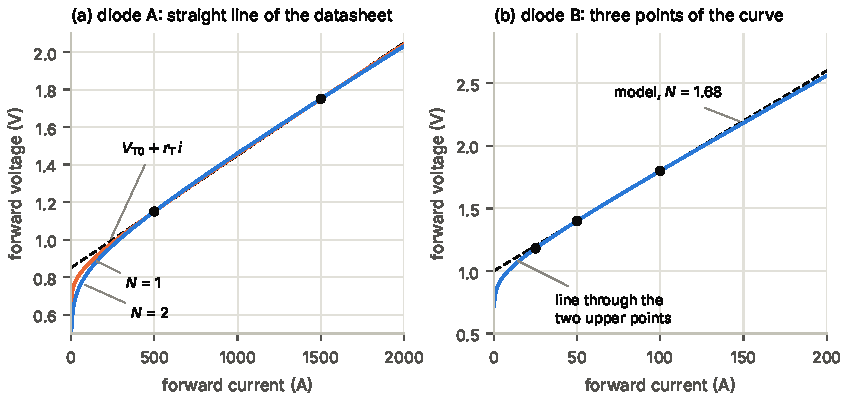
\includegraphics[width=\textwidth]{figures/fig_forward.pdf}
\caption{Forward characteristic of the model against the data. (a) Diode A: straight line of the datasheet (dashed), with its two points, and the secant fit for $\Nem = 1$ and $\Nem = 2$. (b) Diode B: fit through three points of the curve, and the straight line through the two upper points (dashed).}
\label{fig:forward}
\end{figure}

\subsection{Check in a simulated commutation cell}
\label{sec:cell}
The complete model, with the junction capacitance, the leakage and the series resistance, was simulated in the cell of Fig.~\ref{fig:commcell}a with $\Ls = \VR/a$ and an RC snubber (Appendix~\ref{app:scripts}). The junction capacitances are estimates, $\Cjo = \SI{\lmACj}{\nano\farad}$ for A and \SI{\lmBCj}{\nano\farad} for B. Table~\ref{tab:cell} compares the simulation with the closed forms and Fig.~\ref{fig:cell} shows the waveforms.

\begin{table}[htb]
\centering\small
\caption{Simulated commutation cell against the closed forms. The closed forms are evaluated at the slope of the simulation; the charge is integrated down to \SI{\lmPEndPct}{\percent} of the peak, \eqref{eq:qrp}.}
\label{tab:cell}
\begin{tabular}{@{}lcc@{}}
\toprule
 & Diode A & Diode B \\
\midrule
Inductance $\Ls = \VR/a$ & \SI{\lmAL}{\micro\henry} & \SI{\lmBL}{\micro\henry} \\
Snubber $\Rsn$, $\Csn$ & \SI{\lmARsn}{\ohm}, \SI{\lmACsn}{\nano\farad} & \SI{\lmBRsn}{\ohm}, \SI{\lmBCsn}{\nano\farad} \\
Slope at the current zero & \SI{\lmASimSlope}{\ampere\per\micro\second} ($\lmASimSlopeErr\,\%$) & \SI{\lmBSimSlope}{\ampere\per\micro\second} ($\lmBSimSlopeErr\,\%$) \\
\addlinespace
$\Irr$, closed form \eqref{eq:lambert} & \SI{\lmASimIrrCf}{\ampere} & \SI{\lmBSimIrrCf}{\ampere} \\
$\Irr$, simulation, diffusion current & \SI{\lmASimIrrDif}{\ampere} ($\lmASimIrrDifErr\,\%$) & \SI{\lmBSimIrrDif}{\ampere} ($\lmBSimIrrDifErr\,\%$) \\
$\Irr$, simulation, terminals & \SI{\lmASimIrrTerm}{\ampere} ($\lmASimIrrTermErr\,\%$) & \SI{\lmBSimIrrTerm}{\ampere} ($\lmBSimIrrTermErr\,\%$) \\
\addlinespace
$Q_\mathrm{r}$, closed form \eqref{eq:qrp} & \SI{\lmASimQCf}{\micro\coulomb} & \SI{\lmBSimQCf}{\micro\coulomb} \\
$Q_\mathrm{r}$, simulation, terminals & \SI{\lmASimQTerm}{\micro\coulomb} ($\lmASimQTermErr\,\%$) & \SI{\lmBSimQTerm}{\micro\coulomb} ($\lmBSimQTermErr\,\%$) \\
Charge of the junction capacitance, \eqref{eq:qc} & \SI{\lmAQc}{\micro\coulomb} & \SI{\lmBQc}{\micro\coulomb} \\
\addlinespace
$\trr$, straight line, closed form \eqref{eq:trr} & \SI{\lmASimTrrCf}{\micro\second} & \SI{\lmBSimTrrCf}{\nano\second} \\
$\trr$, straight line, simulation & \SI{\lmASimTrr}{\micro\second} & \SI{\lmBSimTrr}{\nano\second} \\
\addlinespace
Peak reverse voltage without capacitance, \eqref{eq:vrm} & \SI{\lmAVpk}{\volt} & \SI{\lmBVpk}{\volt} \\
\quad with the junction capacitance alone, \eqref{eq:vpkcj} & \SI{\pdAVpkCj}{\volt} & \SI{\pdBVpkCj}{\volt} \\
\quad with the junction capacitance alone, simulation & \SI{\pdAVpkCjSim}{\volt} & \SI{\pdBVpkCjSim}{\volt} \\
\quad with the snubber, simulation & \SI{\lmASimVpk}{\volt} & \SI{\lmBSimVpk}{\volt} \\
Energy in the diode after the current zero & \SI{\lmASimEd}{\milli\joule} & \SI{\lmBSimEd}{\milli\joule} \\
Energy in the snubber resistor & \SI{\lmASimEr}{\milli\joule} & \SI{\lmBSimEr}{\milli\joule} \\
Sum & \SI{\lmASimEsum}{\milli\joule} & \SI{\lmBSimEsum}{\milli\joule} \\
Balance $\VR\Qrr + \Csn\VR^2/2$, \eqref{eq:ebal} & \SI{\lmASimEbal}{\milli\joule} & \SI{\lmBSimEbal}{\milli\joule} \\
\bottomrule
\end{tabular}
\end{table}

The table shows four things.
\begin{itemize}
\item The slope at the current zero is a little above $\VR/\Ls$, because the forward voltage of the diode adds to $\VR$ while the current falls. The effect is below one percent here; it grows when $\VR$ is small.
\item The diffusion current of the simulation follows the closed form within \SI{0.5}{\percent}. The current at the terminals is higher at the peak, by \SI{0.1}{\percent} for A and \SI{1.5}{\percent} for B: this is the current of the junction capacitance while the voltage rises. For diode B the charge at the terminals exceeds the closed form by \SI{0.3}{\percent}, which is the charge of the junction capacitance, as the note of the standard says. For diode A that charge is negligible, and the \SI{0.1}{\percent} that remains comes from the slope, which is not exactly constant along the ramp because the forward voltage changes with the current.
\item The recovery time of the straight-line convention is reproduced within \SI{0.6}{\percent}.
\item The energy balance \eqref{eq:ebal} closes within \SI{0.5}{\percent}. Without the snubber the junction capacitance alone would bring the peak of the voltage to about \SI{\pdAVpkCjSim}{\volt} for A and \SI{\pdBVpkCjSim}{\volt} for B, as \eqref{eq:vpkcj} predicts: for diode B far beyond its $\Vrrm$ of \SI{\lmBVrrm}{\volt}. The snubber damps this oscillation. For diode A it is fast against the tail ($\Rsn\Csn = \SI{\lmARsnCsn}{\micro\second}$, $\taurr = \SI{\lmATrr}{\micro\second}$): the peak is \SI{\lmASimVpk}{\volt}, practically the \SI{\lmAVpk}{\volt} that \eqref{eq:vrm} gives without capacitance, and nearly all the energy stays in the diode. For diode B it is as slow as the tail ($\Rsn\Csn = \SI{\lmBRsnCsn}{\nano\second}$, $\taurr = \SI{\lmBTrr}{\nano\second}$): it brings the peak to \SI{\lmBSimVpk}{\volt}, below the \SI{\lmBVpk}{\volt} of \eqref{eq:vrm}, and takes more than half of the energy.
\end{itemize}

\begin{figure}[htb]
\centering
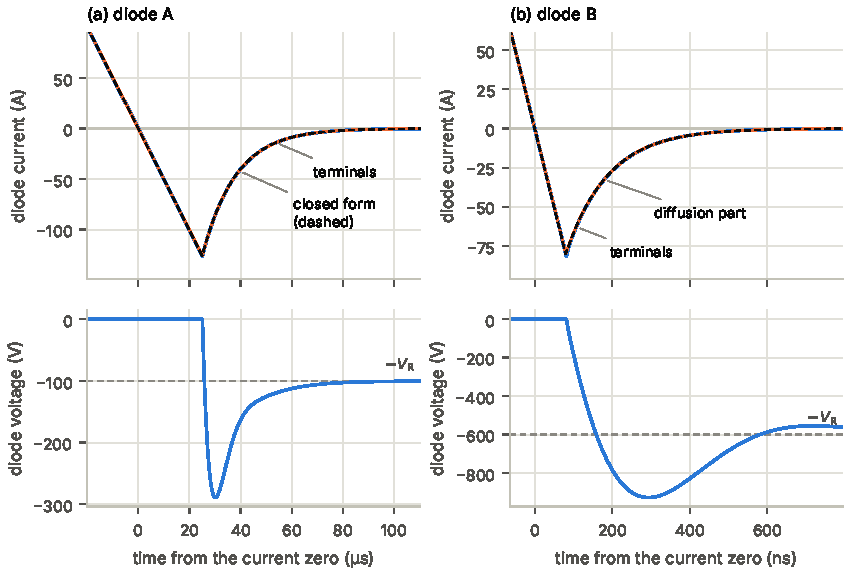
\includegraphics[width=\textwidth]{../lauritzen_ma_datasheet_conversion/figures/fig_cell.pdf}
\caption{Simulated commutation cell with the snubber: current and voltage of the diode. The current at the terminals, the diffusion current and the closed form of Sec.~\ref{sec:ramp} (dashed) lie on each other; for diode B, at the peak, the terminal current slightly exceeds the diffusion current (``diffusion part'' in the figure): the difference is the current of the junction capacitance.}
\label{fig:cell}
\end{figure}

\subsection{Away from the datasheet point}
\label{sec:away}
Table~\ref{tab:awaya} and Fig.~\ref{fig:curves} show the two sets at other slopes and forward currents.

\begin{table}[htb]
\centering\small
\caption{Diode A away from the datasheet point, at $\IF = \SI{\lmAIf}{\ampere}$: the set of Table~\ref{tab:conv} against the assumed curve of the datasheet, and the set that the curve asks for at each slope (curve point converted with the softness of the datasheet point).}
\label{tab:awaya}
\begin{tabular}{@{}lccccc@{}}
\toprule
Slope $a$ [\si{\ampere\per\micro\second}] & \lmAAwayALo & \lmAAwayALoB & \lmAAwayARef & \lmAAwayAHiB & \lmAAwayAHi \\
\midrule
Length of the ramp, $\xi = \Tone/\tau$ & \lmAAwayXALo & \lmAAwayXALoB & \lmAAwayXARef & \lmAAwayXAHiB & \lmAAwayXAHi \\
$\Irr$ of the set [A] & \lmAAwayIrrALo & \lmAAwayIrrALoB & \lmAAwayIrrARef & \lmAAwayIrrAHiB & \lmAAwayIrrAHi \\
$\Qrr$ of the set [\si{\micro\coulomb}] & \num{\lmAAwayQrrALo} & \num{\lmAAwayQrrALoB} & \num{\lmAAwayQrrARef} & \num{\lmAAwayQrrAHiB} & \num{\lmAAwayQrrAHi} \\
$\Qrr$ of the datasheet curve [\si{\micro\coulomb}] & \lmAAwayDsALo & \lmAAwayDsALoB & \lmAAwayDsARef & \lmAAwayDsAHiB & \lmAAwayDsAHi \\
Set over curve & \lmAAwayRatioALo & \lmAAwayRatioALoB & \lmAAwayRatioARef & \lmAAwayRatioAHiB & \lmAAwayRatioAHi \\
\addlinespace
Curve point converted: $\tau$ [\si{\micro\second}] & \lmAAwayTauALo & \lmAAwayTauALoB & \lmAAwayTauARef & \lmAAwayTauAHiB & \lmAAwayTauAHi \\
Curve point converted: $\TM$ [\si{\micro\second}] & \lmAAwayTmALo & \lmAAwayTmALoB & \lmAAwayTmARef & \lmAAwayTmAHiB & \lmAAwayTmAHi \\
\bottomrule
\end{tabular}
\end{table}

For diode A the ramp of the set lasts at least five lifetimes up to \SI{\pdALongSlopeFive}{\ampere\per\micro\second} and three up to \SI{\pdALongSlopeThree}{\ampere\per\micro\second}; at \SI{10}{\ampere\per\micro\second} it lasts \num{\lmAAwayXAHiB} lifetimes, and the long-ramp relations are off by \SI{\pdATenIrrPct}{\percent} on the peak and by \SI{\pdATenQrrPct}{\percent} on the charge. Up to that slope the charge of the set is proportional to the slope, while the curve of the datasheet grows with the exponent \num{\lmAQexp}. A decade below the datasheet point the set has a fifth of the charge of the curve. The last two rows are the sets that reproduce the curve at each slope: the lifetime goes from \SI{\lmAAwayTauALo}{\micro\second} at the lowest slope to \SI{\lmAAwayTauAHi}{\micro\second} at the highest, following \eqref{eq:taucurve} as long as the ramp is long. At the datasheet slope the forward current has almost no effect: \SI{\lmAAwayQrrFLo}{\micro\coulomb} at \SI{\lmAAwayFLo}{\ampere} and \SI{\lmAAwayQrrFHi}{\micro\coulomb} at \SI{\lmAAwayFHi}{\ampere}, against \SI{\lmAQrr}{\micro\coulomb} at \SI{\lmAIf}{\ampere}.

Diode B behaves in the opposite way. At twice the slope the charge grows from \SI{\lmBQrr}{\micro\coulomb} to \SI{\lmBAwayQrrAHi}{\micro\coulomb} only, and at half the slope it falls to \SI{\lmBAwayQrrALo}{\micro\coulomb}; at twice the forward current it is \SI{\lmBAwayQrrFHi}{\micro\coulomb} and at half the forward current \SI{\lmBAwayQrrFLo}{\micro\coulomb}. The peak current goes from \SI{\lmBAwayIrrALo}{\ampere} to \SI{\lmBAwayIrrAHi}{\ampere} over the two slopes and from \SI{\lmBAwayIrrFLo}{\ampere} to \SI{\lmBAwayIrrFHi}{\ampere} over the two currents. The point at half the slope and the point at twice the forward current have the same ratio $\IF/a$, and the second is twice the first, in the peak and in the charge: this is the homogeneity of Sec.~\ref{sec:exponents}.

\begin{figure}[htb]
\centering
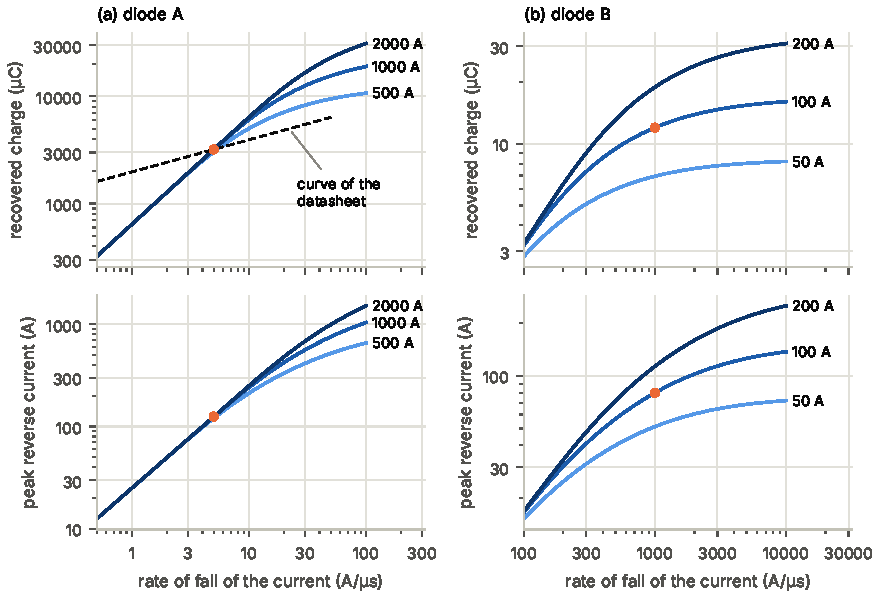
\includegraphics[width=\textwidth]{../lauritzen_ma_datasheet_conversion/figures/fig_curves.pdf}
\caption{The two sets of Table~\ref{tab:conv} at other slopes, for half, one and twice the forward current of the datasheet test. The point is the datasheet point. For diode A the dashed line is the assumed curve of the datasheet.}
\label{fig:curves}
\end{figure}

\subsection{Temperature}
For diode B the datasheet gives the recovery at \SI{\lmBTtwo}{\celsius} as well. The same conversion gives $\taurr = \SI{\lmBTrrTtwo}{\nano\second}$, $\tau = \SI{\lmBTauTtwo}{\nano\second}$ and $\TM = \SI{\lmBTmTtwo}{\nano\second}$: against \SI{\lmBT}{\celsius} the lifetime is lower by \SI{\lmBTauTtwoPct}{\percent} and the transit time by \SI{\lmBTmTtwoPct}{\percent}. The two parameters do not scale together, so the softness changes with the temperature as well.

For diode A there are no data at a second temperature. As an example of the scaling \eqref{eq:scale}, a set with both time constants lower by \SI{\lmAIrrTtwoPct}{\percent} ($\tau = \SI{\lmATauTtwo}{\micro\second}$, $\TM = \SI{\lmATmTtwo}{\micro\second}$) gives at the datasheet slope $\Irr = \SI{\lmAIrrTtwo}{\ampere}$ and $\Qrr = \SI{\lmAQrrTtwo}{\micro\coulomb}$: the peak falls by the same \SI{\lmAIrrTtwoPct}{\percent} and the charge by \SI{\lmAQrrTtwoPct}{\percent}, because it goes with the square of the time constants. In the other direction, a charge known to be lower by \SI{\lmAQrrTtwoPct}{\percent} at a lower temperature asks for time constants lower by \SI{\lmAIrrTtwoPct}{\percent}.

\subsection{The same diodes in other descriptions}
\begin{table}[htb]
\centering\small
\caption{Quantities of the two sets in other conventions and test circuits.}
\label{tab:other}
\begin{tabular}{@{}llcc@{}}
\toprule
Quantity & & Diode A & Diode B \\
\midrule
$\trr$, straight line through \SI{90}{\percent} and \SI{25}{\percent} & \eqref{eq:trr} & \SI{\lmATrrLine}{\micro\second} & \SI{\lmBTrrLine}{\nano\second} \\
$\trr$, current at \SI{10}{\percent} of the peak & \eqref{eq:trr} & \SI{\lmATrrTen}{\micro\second} & \SI{\lmBTrrTen}{\nano\second} \\
$\trr$, triangle of equal charge, $2\Qrr/\Irr$ & & \SI{\lmATrrTri}{\micro\second} & \SI{\lmBTrrTri}{\nano\second} \\
Stretch factor $\trr\,a/\Irr$ (\SI{10}{\percent} convention) & & \lmAStretch & \lmBStretch \\
$\tb/\ta$, straight-line convention & & \lmASLine & \lmBSLine \\
\addlinespace
Abrupt commutation: $\Irr = \IF\tau/\TM$ & \eqref{eq:abrupt} & \SI{\lmAIrrFast}{\ampere} & \SI{\lmBIrrFast}{\ampere} \\
Abrupt commutation: $\Qrr = \IF(\tau-\taurr)$ & \eqref{eq:abrupt} & \SI{\lmAQrrFast}{\micro\coulomb} & \SI{\lmBQrrFast}{\micro\coulomb} \\
Static charge over datasheet charge, $\tau\IF/\Qrr$ & & \lmATauIfRatio & \lmBTauIfRatio \\
\addlinespace
Peak reverse voltage without capacitance, $\VR(1+2/s)$ & \eqref{eq:vrm} & \SI{\lmAVpk}{\volt} & \SI{\lmBVpk}{\volt} \\
Recovery energy $\VR\,\Qrr$ & \eqref{eq:erec} & \SI{\lmAErec}{\milli\joule} & \SI{\lmBErec}{\milli\joule} \\
\bottomrule
\end{tabular}
\end{table}

Table~\ref{tab:other} gives the two sets in the other conventions of Sec.~\ref{sec:direct}. Two more test circuits complete the picture.

\emph{Resistive commutation of diode B.} With $\IF = \SI{\lmBStepIf}{\ampere}$ and $\IR = \SI{\lmBStepIr}{\ampere}$ the ratio $\IF/\IR = \lmBStepRatio$ is below $\TM/\tau = \lmBTmOverTau$: there is no storage phase. The reverse current starts from $\IF\tau/\TM = \SI{\lmBStepIzero}{\ampere}$ and falls to \SI{\lmBStepIrec}{\ampere} in \SI{\lmBStepTrr}{\nano\second}. With $\IF = \SI{\lmBStepIfTwo}{\ampere}$ the storage time \eqref{eq:ts} is \SI{\lmBStepTsTwo}{\nano\second} and the current reaches \SI{\lmBStepIrec}{\ampere} after \SI{\lmBStepTrrTwo}{\nano\second}. A recovery time measured in such a test has little to do with the \SI{\lmBTrrLine}{\nano\second} of the ramp test, and it depends on the two currents of the test.

\emph{Half-sine pulse on diode A.} A half sine of \SI{\lmASineLongMs}{\milli\second} with the slope of the datasheet at its zero has a peak of \SI{\lmASineLongIpk}{\kilo\ampere}; \eqref{eq:sine} gives a peak reverse current that differs by $\lmASineLongErr\,\%$ from the long-ramp value $a(\tau-\taurr) = \SI{\lmALongIrr}{\ampere}$. With a half sine of \SI{\lmASineShortMs}{\milli\second} (peak \SI{\lmASineShortIpk}{\kilo\ampere}, $\omega\tau = \lmASineShortWt$) the difference is $\lmASineShortErr\,\%$. A half-sine test at line frequency and a ramp test with the same slope at the zero are the same test for the model.

\subsection{Sensitivity of the two conversions}
\begin{table}[htb]
\centering\small
\caption{Relative change of the parameters of the exact conversion for a relative change of one datum of one percent (numerical derivatives of \eqref{eq:taurr}, \eqref{eq:iter} and \eqref{eq:tm}).}
\label{tab:sensex}
\begin{tabular}{@{}lcccccc@{}}
\toprule
 & \multicolumn{3}{c}{Diode A} & \multicolumn{3}{c}{Diode B} \\
\cmidrule(lr){2-4}\cmidrule(l){5-7}
Datum & $\tau$ & $\taurr$ & $\TM$ & $\tau$ & $\taurr$ & $\TM$ \\
\midrule
$\Qrr$ & $\lmASensTauQ$ & $\lmASensTrrQ$ & $\lmASensTmQ$ & $\lmBSensTauQ$ & $\lmBSensTrrQ$ & $\lmBSensTmQ$ \\
$\Irr$ & $\lmASensTauI$ & $\lmASensTrrI$ & $\lmASensTmI$ & $\lmBSensTauI$ & $\lmBSensTrrI$ & $\lmBSensTmI$ \\
$a$ & $\lmASensTauA$ & $\lmASensTrrA$ & $\lmASensTmA$ & $\lmBSensTauA$ & $\lmBSensTrrA$ & $\lmBSensTmA$ \\
$\IF$ & $\lmASensTauF$ & $\lmASensTrrF$ & $\lmASensTmF$ & $\lmBSensTauF$ & $\lmBSensTrrF$ & $\lmBSensTmF$ \\
\bottomrule
\end{tabular}
\end{table}
For diode A the numbers of Table~\ref{tab:sensex} are those of \eqref{eq:sens} with $s = \lmAS$ within \num{0.01}, and the forward current has no weight. A peak current higher by \SI{5}{\percent} at the same charge moves $\tau$ by $\lmAFiveTau\,\%$, $\taurr$ by $\lmAFiveTrr\,\%$ and $\TM$ by $\lmAFiveTm\,\%$. For diode B the same change gives $\lmBFiveTau\,\%$, $\lmBFiveTrr\,\%$ and $\lmBFiveTm\,\%$. On its short ramp the lifetime depends on the forward current of the test almost as much as on the peak current, and hardly on the slope: the forward current of the datasheet test has to be known and used.

%=====================================================================
\section{Procedure}
\label{sec:procedure}
\begin{enumerate}
\item \emph{Choose the data.} Take $\Irr$ and $\Qrr$ at the temperature of interest and at the slope nearest to that of the application, with the forward current, the slope and the reverse voltage of the test. Note whether they are maximum or typical values and which convention defines the recovery time, if it is used (Table~\ref{tab:kappa}).
\item \emph{Check the pair.} The charge has to exceed the triangle: $\Qrr > \Irr^2/(2a)$. Compute $\Irr/\IF$: below \num{0.1}, with a softness up to 2, the ramp of the test is long; above, it may not be (Table~\ref{tab:valid}).
\item \emph{Tail time constant.} $\taurr = \Qrr/\Irr - \Irr/(2a)$, \eqref{eq:taurr}; from other pairs, with \eqref{eq:fromtrr}--\eqref{eq:fromq}.
\item \emph{Lifetime.} Iterate \eqref{eq:iter} from $\tau = \taurr + \Irr/a$. On a long ramp the starting value is the result.
\item \emph{Transit time.} $\TM = \tau\taurr/(\tau-\taurr)$, \eqref{eq:tm}. The softness of the diode on a long ramp is $2\TM/\tau$.
\item \emph{Conduction.} Choose $\Nem$ (2 for a power diode in high injection) and fit $\IS$ and $\RS$ to the straight line, \eqref{eq:tangent} or \eqref{eq:secant}, or fit all three to points of the curve, \eqref{eq:points}. Multiply $\IS$ by $(\tau+\TM)/\tau$ if the implementation writes the junction law with $\tau\,\IS^{*}$.
\item \emph{Blocking.} $\Rr$ from the reverse current at the working voltage and temperature; $\Cjo$ from the datasheet, \eqref{eq:cj}, or from an estimate with \eqref{eq:wsc} (Sec.~\ref{sec:blocking}). If the charge \eqref{eq:qc} is not small against $\Qrr$, subtract it from the datasheet charge and repeat steps 3--5.
\item \emph{Verify.} Put the set on the test ramp, with \eqref{eq:lambert} or with a simulation of the test cell, and compare $\Irr$, $\Qrr$ and $\trr$ with the datasheet. Then look at the working point of the application: slope, forward current and length of the ramp in lifetimes. If the slope is far from that of the data, convert again from the nearest point of the datasheet curve (Sec.~\ref{sec:slope}).
\item \emph{Bracket.} Where the result depends on the softness (peak voltage, damping) or on the spread between devices, repeat with $\TM$ at the ends of its range (Sec.~\ref{sec:sens}) and with the scaled set \eqref{eq:scale}, which holds on a long ramp.
\end{enumerate}

%=====================================================================
\part{Technology and application}

\section{Device technologies}
\label{sec:technology}
\subsection{What can be optimised}
A power diode is judged on four quantities: the voltage it blocks, the forward voltage, the charge and the current of the recovery, the softness. The results of Parts~I and~II say what ties them together.
\begin{itemize}
\item \emph{The base is set by the voltage.} Width and doping follow from the breakdown voltage (Sec.~\ref{sec:why}); a punch-through base with a buffer is about one third thinner than a non-punch-through one.
\item \emph{For a given base, charge and drop trade against each other.} The product $\VM\,\QF$ of \eqref{eq:tradeoff} does not depend on the lifetime and grows with the square of the base width: every reduction of the stored charge obtained by shortening the lifetime is paid for in forward voltage.
\item \emph{A lifetime longer than the one that gives $\La \approx d$ is of no use.} At a fixed current the forward voltage has a flat minimum around $d/\La \approx \num{\pdVfMinBeta}$ (Sec.~\ref{sec:vf}): a longer lifetime adds charge without removing voltage.
\item \emph{Where the plasma sits matters.} The plasma next to the \Pp\Nm{} junction sets the peak reverse current, the one on the cathode side feeds the tail (Sec.~\ref{sec:softsnappy}). The natural catenary \eqref{eq:catenary} has more plasma on the anode side, \eqref{eq:edges}, because of the ratio of the mobilities: it is the wrong distribution for the recovery.
\end{itemize}
The technologies that follow act on one of these points. The descriptions are qualitative and quoted from memory [M]~\cite{lutz,baliga}.

\subsection{Lifetime control}
\label{sec:lifetimecontrol}
\emph{Uniform.} Recombination centres are introduced in the whole volume: by diffusion of gold or of platinum, or by electron irradiation. Gold has a level close to mid-gap: it gives the best trade-off between forward voltage and charge, but also the highest generation, hence a high leakage that limits the voltage and the junction temperature (Sec.~\ref{sec:blockingphys}). Platinum has a level far from mid-gap: the leakage stays low, but the lifetime grows strongly with the temperature, and with it the recovered charge; the temperature coefficient of the forward voltage usually stays negative up to the rated current (Sec.~\ref{sec:temperature}). Electron irradiation gives a leakage about twice that of platinum, hence well below that of gold, but the least favourable trade-off between forward voltage and charge of the three \cite{baligasun1977}; in return it is adjusted with precision on the finished device.

\emph{Local.} The implantation of protons or of helium ions creates a zone of low lifetime at a chosen depth. Placed next to the \Pp\Nm{} junction, it lowers the plasma where it has to be removed first and leaves it on the cathode side: $\Irr$ falls and the tail remains. It is the principle of the \emph{controlled axial lifetime} (CAL) diodes, which combine it with a uniform irradiation.

\subsection{Efficiency of the emitters}
\label{sec:emittereff}
As an alternative to the recombination centres the injection from the anode can be reduced. A lightly doped or thin \Pp{} emitter has a high parameter $h_\mathrm{p}$: by \eqref{eq:bcem} the concentration at the \Pp\Nm{} edge grows only with the square root of the current, and the profile is inverted, lower at the anode than at the cathode. It is the principle of the \emph{emitter controlled} diodes. Since the lifetime of the base stays long, the leakage is low. The plasma is limited by the emitter, not by centres whose lifetime grows with the temperature, and the drop on the base, which the weak emitter makes higher (Sec.~\ref{sec:emitter}), rises with the temperature because the mobilities fall (Sec.~\ref{sec:temperature}): the temperature coefficient of the forward voltage becomes positive already at moderate currents, which helps the parallel connection. The \emph{merged PIN--Schottky} (MPS) structure, in which Schottky zones interrupt the \Pp{} emitter, has the same purpose.

\subsection{Base, buffer and field stop}
\label{sec:buffer}
An n-type buffer between the base and the \Np{} emitter stops the field, and allows a thinner base at the same breakdown voltage, \eqref{eq:pt}: \SI{\pdPtSavePct}{\percent} less in the example of Sec.~\ref{sec:why}. Since the drop on the base and the product \eqref{eq:tradeoff} go with $\wB^2$, it is the most effective way of reducing the forward voltage and the charge together.

The price is the softness. In a thin base the space charge region reaches the buffer before the plasma on the cathode side is exhausted, and the current is interrupted abruptly (Sec.~\ref{sec:softsnappy}). A diode with a field stop is soft only if the buffer is deep and lightly doped, so as to retain charge, or if other measures keep plasma at the cathode until the end: the control of the anode already described, or structures that inject holes from the cathode during the recovery.

\subsection{Silicon carbide}
\label{sec:sic}
The critical field of 4H-SiC is about ten times that of silicon. At the same voltage the base can be ten times thinner and a hundred times more heavily doped, and the resistance \eqref{eq:runi} of a base without injection falls by two or three orders of magnitude. A \SI{1200}{\volt} unipolar silicon diode would have $R_\mathrm{B} \approx \SI{\pdSiUniR}{\ohm\centi\metre\squared}$, that is \SI{\pdSiUniDrop}{\volt} at \SI{100}{\ampere\per\centi\metre\squared}; in silicon carbide the same voltage is blocked with a base of about \SI{1}{\milli\ohm\centi\metre\squared}. Up to a few kilovolts the conductivity modulation is therefore not needed: the diode can be a \emph{Schottky diode}, without plasma and without stored charge.

A silicon carbide Schottky diode has no reverse recovery in the sense of this document. At turn-off only the current that charges the junction capacitance flows, with the charge $Q_\mathrm{c}$ of \eqref{eq:qc}: it does not depend on the forward current, on the slope or on the temperature, and it is lower by an order of magnitude or more than the $\Qrr$ of a silicon fast diode of the same voltage and current [M]. The forward voltage has a threshold close to one volt and a positive temperature coefficient, dominated by the mobility. The commercial structures are MPS: the \Pp{} zones shield the Schottky contact from the field and, at overload currents, inject holes and bring the diode into bipolar conduction. It is the remedy for the weak point of the unipolar diode, the overload capability: without injection the forward voltage grows with the current and with the temperature, and the allowed surge current, with its $I^2t$, stays below that of a silicon PIN diode of the same rated current [M]. The other limit is the cost. Table~\ref{tab:sic} summarises the comparison.

\begin{table}[htb]
\centering\small
\caption{Silicon and silicon carbide diodes: indicative orders of magnitude for \SI{1200}{\volt} devices, quoted from memory [M] and to be checked on the datasheets.}
\label{tab:sic}
\begin{tabular}{@{}lccc@{}}
\toprule
 & Si PIN rectifier & Si PIN fast & SiC Schottky (MPS) \\
\midrule
Conduction & bipolar & bipolar & unipolar \\
Lifetime of the base & \SIrange{10}{100}{\micro\second} & \SIrange{0.1}{1}{\micro\second} & no plasma \\
$\VF$ at the rated current, \SI{25}{\celsius} & \SIrange{1.0}{1.3}{\volt} & \SIrange{1.5}{2.5}{\volt} & \SIrange{1.4}{1.8}{\volt} \\
Temperature coefficient of $\VF$ & negative & depends on the technology & positive \\
Charge at turn-off & $\Qrr$, part of $\tau\IF$ & $\Qrr$, part of $\tau\IF$ & only $Q_\mathrm{c}$ \\
Dependence of the charge on the slope and $\Tj$ & strong & strong & none \\
Overload capability ($I^2t$) & excellent & good & limited \\
\bottomrule
\end{tabular}
\end{table}

Above a few kilovolts the base without injection becomes too resistive in silicon carbide as well, and the PIN structure comes back. The physics is that of Parts~I and~II with other numbers: a band gap of about \SI{3.3}{\electronvolt}, hence junction voltages around \SI{3}{\volt}, and lifetimes of a few microseconds.

%=====================================================================
\section{The diode in the converter}
\label{sec:converter}
\subsection{Losses}
\label{sec:losses}
\emph{Conduction.} With the straight line \eqref{eq:line} the average power in conduction is $P = \VTo\,I_\mathrm{AV} + \rT\,I_\mathrm{RMS}^2$, where $I_\mathrm{AV}$ and $I_\mathrm{RMS}$ are the average value and the rms value of the diode current.

\emph{Switching.} In a switching leg the recovery of the freewheeling diode is paid for twice (Sec.~\ref{sec:switchingleg}): in the diode, which dissipates $\Erec$ during the tail, and in the switch that turns on, which during $\ta$ carries the current of the load plus the reverse current at full voltage. For diode B of Sec.~\ref{sec:examples} at its datasheet point (\SI{\lmBVr}{\volt}, \SI{\lmBIf}{\ampere}, \SI{\lmBSlope}{\ampere\per\micro\second}, $\Irr = \SI{\lmBIrr}{\ampere}$, $\ta = \SI{\lmBTa}{\nano\second}$, $s = \lmBS$):
\begin{itemize}
\item the source delivers for the recovery $\Vdc\,\Qrr = \SI{\pdSwErecIdeal}{\milli\joule}$;
\item with $\Ls a \ll \Vdc$ and the switch already in full conduction during the tail, the diode dissipates the part $s/(1+s) = \num{\pdSwK}$ of it, that is $\Erec \approx \SI{\pdSwErecDiode}{\milli\joule}$, \eqref{eq:erecleg}; with a real switch, which still sustains a part of the voltage, it is less;
\item the turn-on energy of the switch grows by $\Delta E_\mathrm{on} \approx \SI{\pdSwEonExtra}{\milli\joule}$, \eqref{eq:eon}: \SI{\pdSwEonLoad}{\milli\joule} for the current of the load carried at full voltage for the extra time $\ta$, and \SI{\pdSwEonQa}{\milli\joule} for the reverse current.
\end{itemize}
The recovery costs the switch \num{\pdSwRatio} times what it costs the diode. This is why a diode without stored charge reduces above all the turn-on losses of the switch, and why $\Erec$ alone underestimates the benefit. The switching losses are then the sum of the energies times the frequency, $P = f_\mathrm{sw}\,(E_\mathrm{on} + E_\mathrm{off} + \Erec)$, with energies read or measured at the voltage, at the current, at the slope and at the temperature of the application.

\subsection{di/dt, stray inductance and overvoltage}
The commutation slope is a choice of the design, through the drive of the switch (in an IGBT or in a MOSFET, the gate resistance). A steeper slope reduces the turn-on energy of the switch itself, but increases $\Irr$, moves the blocking instant earlier, to a larger residual charge, and makes the tail steeper: the overvoltage $2\Ls a/s$ of \eqref{eq:vrmleg}, the risk of snap-off and that of dynamic avalanche grow (Secs.~\ref{sec:softsnappy} and~\ref{sec:dynaval}). With $\Ls = \SI{\pdSwLs}{\nano\henry}$ and \SI{\lmBSlope}{\ampere\per\micro\second} the overvoltage is \SI{\pdSwOvSoft}{\volt} for the softness of diode B and \SI{\pdSwOvSnap}{\volt} for a diode with $s = \num{\pdSwSnapS}$; in the cell with an ideal switch, where the same inductance sets the slope, it would be \SI{\pdSwOvIdeal}{\volt}, \eqref{eq:vrm}. On these values the oscillation of the stray inductance with the capacitances of the diode and of the switch is superimposed (Sec.~\ref{sec:switchingleg}). The overvoltage is proportional to the stray inductance: the layout of the commutation loop matters as much as the choice of the diode.

\subsection{Snubber, series and parallel}
\emph{Snubber.} Where the same inductance sets the slope and is subjected to the tail (line-commutated converters, thyristors, test cells) the peak reverse voltage \eqref{eq:vrm}, which the junction capacitance alone can almost triple, \eqref{eq:vpkcj}, is not acceptable without an RC snubber across the diode, which damps the oscillation; the balance \eqref{eq:ebal} gives its losses, and Sec.~\ref{sec:cell} a simulated example. Switching legs with IGBTs or MOSFETs normally work without snubber: there the voltage $\Vdc$ appears across the diode at the rate set by the switch, not as a step (Sec.~\ref{sec:switchingleg}), and they rely on the softness of the diode and on a low stray inductance.

\emph{Series.} Diodes in series share the voltage according to their recovered charge: the one with less charge blocks first and takes up the voltage until the others have finished. With a capacitor $C$ across each diode the imbalance is $\Delta V \approx \Delta\Qrr/C$, where $\Delta\Qrr$ is the spread of the charge: it is the relation that sizes the sharing snubbers. In the blocking state the sharing is instead set by the reverse currents, which differ from one device to another and depend strongly on the temperature (Sec.~\ref{sec:blockingphys}): sharing resistors across each diode are also needed, sized to carry a few times the reverse current of the device \cite{dynexan6531,stan443}.

\emph{Parallel.} Diodes in parallel share the current according to their forward characteristic. The sharing is stable if the temperature coefficient of the forward voltage is positive at the working current (Sec.~\ref{sec:temperature}).

\subsection{Measurement and model}
The reference test for the recovery in a switching leg is the \emph{double pulse test}: a first pulse brings the current of the load to the desired value, and at the second pulse the switch turns on against the conducting diode. In it $\Irr$, $\Qrr$, $\Erec$ and the overvoltage are measured at the slope, at the voltage and at the temperature of the application. They are also the right data for the model: a parameter set of the two-charge model reproduces the recovery at one point only (Sec.~\ref{sec:slope}), and has to be extracted where the converter works, not where the datasheet was measured.

For a rectifier diode at line frequency the ramp lasts many lifetimes, and the model works in the long-ramp limit \eqref{eq:long}: the recovery does not depend on the forward current, and the closed form \eqref{eq:longinv} is enough for the conversion. The rule, however, does not change: the set is good near the slope at which it was converted, a few amperes per microsecond in the datasheet test, while a transformer-fed bridge with a DC current of up to a few hundred amperes commutates at a fraction of an ampere per microsecond. Below the range of the datasheet curve the set gives too low a charge, proportional to the slope, and the extrapolated curve too high a charge (Sec.~\ref{sec:slope}): the note \texttt{research/diode-stack} (in its Sec.~6) treats this case and gives a floor and a ceiling of the charge.

%=====================================================================
\section{Summary}
\label{sec:summary}
Table~\ref{tab:summary} collects the main relations of the document.

\begin{table}[htb]
\centering\small
\caption{The quantities of the power diode, the relations that set them and what the design can act on.}
\label{tab:summary}
\begin{tabular}{@{}l>{\raggedright\arraybackslash}p{6.6cm}>{\raggedright\arraybackslash}p{5.2cm}@{}}
\toprule
Quantity & Relation & Lever \\
\midrule
Breakdown voltage & $\Vbr \propto \ND^{-3/4}$, $w \propto \ND^{-7/8}$, \eqref{eq:nptlaw} & doping and width of the base, buffer \\
Stored charge & $\QF = \tau\,\IF$, \eqref{eq:qf} & lifetime, efficiency of the emitters \\
Drop on the base & $\VM \approx 2\VT\,(d/\La)^2$, \eqref{eq:vmthin}; exact \eqref{eq:vm} & base width, lifetime \\
Forward voltage & $\VF = \vjo + \VM + \vjt$, \eqref{eq:vfsum}; minimum for $d \approx \La$ & $d/\La$ between \num{\pdVfFlatLo} and \num{\pdVfFlatHi} \\
Charge at the current zero & $a\,\tau^2\,\bigl(1-e^{-\IF/(a\tau)}\bigr)$, \eqref{eq:qzero} & lifetime, slope \\
Peak reverse current & $\Irr = a\,(\tau-\taurr)\,\bigl(1-e^{-\Tone/\tau}\bigr)$, \eqref{eq:peak} & lifetime, plasma at the anode, slope \\
Recovered charge & $\Qrr = \Irr^2/(2a) + \Irr\,\taurr$, \eqref{eq:qrr} & lifetime, slope \\
Softness & $s = 2\taurr/\ta$; $2\TM/\tau$ on a long ramp, \eqref{eq:softlong} & plasma at the cathode, buffer \\
Peak reverse voltage & without capacitance $\VR\,(1+2/s)$, \eqref{eq:vrm}; in a switching leg $\Vdc + 2\Ls a/s$, \eqref{eq:vrmleg} & softness, stray inductance, snubber \\
Recovery energy & $\VR\,\Qrr$, \eqref{eq:erec}; $\approx \Vdc\,\Qrr\,s/(1+s)$, \eqref{eq:erecleg} & charge, softness \\
Turn-on of the switch & $\Delta E_\mathrm{on} \approx \Vdc\,(I_\mathrm{L} + \Irr/2)\,\ta$, \eqref{eq:eon} & $\Irr$, slope \\
\bottomrule
\end{tabular}
\end{table}

In short. A power diode blocks the voltage with a wide and lightly doped base, which by itself would be too resistive to conduct: it conducts because the two emitters fill it with plasma. The same charge that lowers the forward voltage has to be removed at every turn-off, and the product of the drop on the base and the stored charge is set by the base width: there is no lifetime that improves both. The quantity of charge decides the losses; its distribution in the base decides the peak, the tail and the overvoltage. A model with one charge describes the first, one with two charges the second as well, at one working point; what is left out (the dependence of the effective lifetime on the current, the snap-off, the dynamic avalanche) is the reason why a diode must always be checked in the conditions of the application.
%=====================================================================
\appendix
\section{Proofs}
\label{app:proofs}
\subsection{Closed form of the peak}
\label{app:lambert}
Write the first of \eqref{eq:norm} as $y = c - c\,e^{-\lambda}e^{-y}$ with $c = 1-\rho$, and put $z = y - c$. Then $z = -c\,e^{-(\lambda+c)}\,e^{-z}$, that is
\begin{equation}
z\,e^{z} = -c\,e^{-(\lambda+c)} .
\end{equation}
The right-hand side lies between $-1/e$ and zero, because $c\,e^{-c} \leq 1/e$. Since $0 < y < c < 1$, $z$ lies between $-1$ and zero, which is the range of the principal branch: $z = W_0(-c\,e^{-(\lambda+c)})$, and \eqref{eq:lambert} follows.

\subsection{Convergence of the iteration}
\label{app:contraction}
Let $g(\tau) = \taurr + \ta/(1-e^{-\Tone/\tau})$ be the right-hand side of \eqref{eq:iter}, for $\tau > 0$. With $\xi = \Tone/\tau$ its derivative is
\begin{equation}
g'(\tau) = \frac{\ta}{\Tone}\,\frac{\xi^2\,e^{-\xi}}{(1-e^{-\xi})^2} = \frac{\ta}{\Tone}\left(\frac{\xi/2}{\sinh(\xi/2)}\right)^{2} .
\end{equation}
The bracket lies between zero and one, so
\begin{equation}
0 < g'(\tau) < \frac{\ta}{\Tone} = \frac{\Irr}{\IF+\Irr} < 1 .
\end{equation}
The map $g$ is a contraction on the whole half line: it has one fixed point, the iteration converges to it from any starting value, and the error shrinks at each step by a factor smaller than $\Irr/(\IF+\Irr)$. Since $g$ is increasing and $g(\taurr+\ta) > \taurr+\ta$, the sequence that starts from the closed form rises monotonically to the solution: the closed form always underestimates the lifetime. On a long ramp the bracket is very small and two or three steps are enough; when $\Irr$ is close to $\IF$ and the ramp is short the factor is close to one half. The solution exists for every $\taurr > 0$, so the only condition on the data is $\Qrr > \Irr^2/(2a)$. The transit time \eqref{eq:tm} is positive because the solution has $\tau > \taurr + \ta$.

\subsection{Exponents}
\label{app:exponents}
Differentiating the first of \eqref{eq:norm} with respect to $\lambda$, with $(1-\rho)\,e^{-(\lambda+y)} = 1-\rho-y$, gives
\begin{equation}
\frac{\diff y}{\diff\lambda} = \frac{1-\rho-y}{\rho+y} .
\end{equation}
With $\Irr = a\tau\,y(\lambda)$ and $\lambda = \IF/(a\tau)$, $\partial\ln\Irr/\partial\ln a = 1 - (\lambda/y)\,\diff y/\diff\lambda$, which is the first of \eqref{eq:exponents}; the second follows in the same way from $\Qrr = a\tau^2\,(y^2/2+\rho y)$. The derivatives with respect to $\ln\IF$ are $(\lambda/y)\,\diff y/\diff\lambda$ and its counterpart for the charge, so the sums are one, \eqref{eq:euler}.

\subsection{Derivation of the drop on the modulated base}
\label{app:vm}
Integrate the field \eqref{eq:fieldhl} over the base. The second term gives $-B\,\VT\ln[p(d)/p(-d)]$, which with \eqref{eq:edges} is the second term of \eqref{eq:vm}. For the first, write the catenary \eqref{eq:catenary} as a single hyperbolic cosine,
\begin{equation}
p(x) = p_\mathrm{m}\,\cosh\frac{x - x_\mathrm{m}}{\La} , \qquad \tanh\frac{x_\mathrm{m}}{\La} = B\,\tanh\beta , \qquad
p_\mathrm{m} = \frac{\tau\,J}{2\,q\,\La}\,\frac{K}{\sinh\beta} , \qquad K = \sqrt{1 - B^2\tanh^2\beta} ,
\end{equation}
where $x_\mathrm{m}$ is the position of the minimum and $p_\mathrm{m}$ its value. Since the antiderivative of $1/\cosh u$ is $\arctan(\sinh u)$,
\begin{equation}
\frac{J}{q\,(\mun+\mup)}\int_{-d}^{d}\frac{\diff x}{p}
= \frac{J\,\La}{q\,(\mun+\mup)\,p_\mathrm{m}}\,\bigl[\arctan\sinh(\beta - u_\mathrm{m}) + \arctan\sinh(\beta + u_\mathrm{m})\bigr] , \qquad u_\mathrm{m} = \frac{x_\mathrm{m}}{\La} .
\end{equation}
The factor in front of the bracket is $\VT\,(1-B^2)\,\sinh\beta/K$, because $\Da/(\mun+\mup) = \VT\,(1-B^2)/2$. The sum of the two arctangents reduces to a single one: with $\sinh(\beta-u)\sinh(\beta+u) = \sinh^2\beta - \sinh^2 u$ and $\cosh^2 u_\mathrm{m} = 1/K^2$, the tangent of the sum is $2K\sinh\beta/(1 - K^2\sinh^2\beta)$, that is the tangent of $2\arctan(K\sinh\beta)$. Equation \eqref{eq:vm} follows:
\begin{equation}
\frac{\VM}{\VT} = 2\,(1-B^2)\,\frac{\sinh\beta}{K}\,\arctan\bigl(K\sinh\beta\bigr) + B\,\ln\frac{1 + B\tanh^2\beta}{1 - B\tanh^2\beta} .
\end{equation}
For $\beta \ll 1$ the arctangent is equal to its argument and the logarithm to $2B\beta^2$: the two terms are $2\,(1-B^2)\,\beta^2$ and $2B^2\beta^2$, and the sum is $2\beta^2$ for any ratio of the mobilities, \eqref{eq:vmthin}. For $\beta \gg 1$ the arctangent tends to $\pi/2$ and $K$ to $\sqrt{1-B^2}$: the first term tends to $(\pi/2)\sqrt{1-B^2}\,e^{\beta}$, \eqref{eq:vmwide}, and the second to the constant $B\ln b$.
%=====================================================================
\section{Scripts}
\label{app:scripts}
The numbers and the plots of the document are produced by Python scripts, which need NumPy, SciPy and Matplotlib only; the diagrams (Figs.~\ref{fig:bands}--\ref{fig:doubleinj}, \ref{fig:commcell}, \ref{fig:recovery} and~\ref{fig:model}) are drawn in the source.
\begin{itemize}
\emergencystretch=3em\raggedright
\item \texttt{power\_diode\_fundamentals\_calc.py}, in this folder, computes the numbers of Part~I and of the sections that tie the physics to the model: the design of the base for the blocking state, the catenary profile, the drop on the base in exact form and in its approximations, the junction voltages, the recombination in the emitters, the solutions of the charge-control model, the distributed base on a current ramp and, for the two examples, the check of the base width and the peak reverse voltage with the junction capacitance alone. It produces the log \texttt{power\_diode\_fundamentals\_results.txt}, the file \texttt{power\_diode\_fundamentals\_values.tex} with every number quoted as a macro, and the plots of Figs.~\ref{fig:profile}, \ref{fig:vm} and~\ref{fig:forward} in two versions: \texttt{figures/fig\_profile.pdf}, \texttt{fig\_vm.pdf} and \texttt{fig\_forward.pdf}, with English labels, and the same files with the suffix \texttt{\_it}, with Italian labels, for the Italian version of this document (\texttt{power\_diode\_fundamentals\_it.tex}).
\item \texttt{lm\_conversion.py}, in the neighbouring folder \texttt{lauritzen\_ma\_datasheet\_conversion}, is a module with the relations of the two-charge model in SI units: the ramp solution (\texttt{ramp\_recovery}, \texttt{ramp\_peak\_norm}, \texttt{ramp\_exponents}, \texttt{ramp\_waveform}), the conventions of the recovery time (\texttt{trr\_factor}), the other test circuits (\texttt{step\_recovery}, \texttt{sine\_peak}), the conversions (\texttt{lm\_from\_irr\_qrr}, \texttt{lm\_from\_irr\_trr}, \texttt{irr\_from\_qrr\_trr}, \texttt{irr\_from\_qrr\_softness}, \texttt{sensitivities}), the forward fits (\texttt{forward\_tangent}, \texttt{forward\_secant}, \texttt{forward\_points}), the junction capacitance, and the simulation of the commutation cell with the tools to read a waveform as a datasheet would (\texttt{simulate\_cell}, \texttt{measure}). Run as a program it tests the closed forms against a step-by-step integration.
\item \texttt{lm\_conversion\_calc.py}, in the same folder, holds the data of the two diodes of the examples at its top and produces the numbers of Secs.~\ref{sec:ramp}--\ref{sec:examples} and the plots taken from the source note (Figs.~\ref{fig:waveform}, \ref{fig:map}, \ref{fig:inversion}, \ref{fig:cell} and~\ref{fig:curves}): the log \texttt{lm\_conversion\_results.txt}, the file \texttt{lm\_conversion\_values.tex} and the plots, \texttt{figures/fig\_*.pdf} with English labels and the same files with the suffix \texttt{\_it} with Italian labels. This document reads the values file and the English plots from their folder, without copying them. To convert another diode, replace the data of one of the two dictionaries.
\end{itemize}
The two calculation scripts run in less than a minute. The first imports the two modules of the neighbouring folder, and reports if the values file found there is not up to date.

\emph{Distributed base on a ramp.} The results of Sec.~\ref{sec:onenumber} come from the closed-form solution of \eqref{eq:diffusion} with the boundary conditions \eqref{eq:bc}. For a sinusoidal current of amplitude $J$ the profile is $\tau J\,g(x;\gamma)/(q\La)$, with
\begin{equation}
g(x;\gamma) = \frac{\cosh(\gamma x/\La)}{2\,\gamma\,\sinh(\gamma\beta)} - B\,\frac{\sinh(\gamma x/\La)}{2\,\gamma\,\cosh(\gamma\beta)} , \qquad \gamma = \sqrt{1+j\omega\tau} :
\label{eq:gprofile}
\end{equation}
for $\gamma = 1$ it is the catenary \eqref{eq:catenary}, and at $x = -d$ it gives \eqref{eq:edgeresponse}. On a long ramp the current is linear in time and the transient of the start of the ramp has died out: the profile is then, exactly,
\begin{equation}
p(x,t) = \frac{\tau}{q\,\La}\left[J(t)\,g_0(x) + \tau\,\frac{\diff J}{\diff t}\,g_1(x)\right] , \qquad g_0 = g(x;1) , \qquad g_1 = \frac12\,\dpar{g}{\gamma}\bigg|_{\gamma=1} ,
\label{eq:rampprofile}
\end{equation}
and the junction blocks when it vanishes at $x = -d$: this is \eqref{eq:tadist}. On a ramp that starts from the steady state the transient is added, a series of the modes $\cos[n\pi(x+d)/(2d)]$ that decay with the time constants $[1/\tau + n^2\pi^2\Da/(4d^2)]^{-1}$, and the blocking instant is found numerically.

The charge of the tail does not need an integration in time. After blocking the profile still obeys \eqref{eq:diffusion}, with $p(-d) = 0$ and the gradients at the two edges in the ratio $b$, and tends to zero. Its integral in time, $P(x) = \int_{\Tone}^{\infty} p\,\diff t$, therefore satisfies
\begin{equation}
\La^2\,\frac{\diff^2 P}{\diff x^2} - P = -\tau\,p(x,\Tone) , \qquad P(-d) = 0 , \qquad \frac{\diff P}{\diff x}\bigg|_{d} = -\frac1b\,\frac{\diff P}{\diff x}\bigg|_{-d} ,
\label{eq:tailintegral}
\end{equation}
and the charge of the tail is $2\,q\,A\,\Dp$ times the gradient of $P$ at $x = -d$, by the first of \eqref{eq:bc}. Multiplying \eqref{eq:tailintegral} by $\cosh[(d-x)/\La]$ and integrating over the base gives
\begin{equation}
Q_\mathrm{tail} = \frac{2}{1+B}\;\frac{q\,A}{\cosh 2\beta + 1/b}\int_{-d}^{d} p(x,\Tone)\,\cosh\frac{d-x}{\La}\,\diff x ,
\label{eq:qtail}
\end{equation}
a quadrature on the profile at blocking; the softness is $s = 2\,Q_\mathrm{tail}/(\Irr\,\ta)$. The script checks these results with a finite-difference integration of \eqref{eq:diffusion} on a ramp of five lifetimes, with equal mobilities and with those of silicon: the charge left in the base at blocking and the charge of the tail agree with the closed form within \SI{0.3}{\percent}.

\emph{Commutation cell.} The cell of Fig.~\ref{fig:commcell}a has four states: the current $i_\mathrm{sw}$ of the switch, the middle charge, the junction voltage and the voltage $v_\mathrm{c}$ of the snubber capacitor,
\begin{equation}
\begin{aligned}
\Ls\,\frac{\diff i_\mathrm{sw}}{\diff t} &= \VR + v , &\qquad \frac{\diff\qM}{\diff t} &= \frac{\qE-\qM}{\TM} - \frac{\qM}{\tau} , \\
\Cj(\vj)\,\frac{\diff\vj}{\diff t} &= i - \frac{\qE-\qM}{\TM} - \frac{\vj}{\Rr} , &\qquad \Csn\,\frac{\diff v_\mathrm{c}}{\diff t} &= \frac{v - v_\mathrm{c}}{\Rsn} ,
\end{aligned}
\end{equation}
with $i = \IF - i_\mathrm{sw} - (v-v_\mathrm{c})/\Rsn$, $v = \vj + \RS\,i$ and $\qE$ from \eqref{eq:qe}. The system is stiff, because the junction voltage reacts much faster than the charge; it is integrated with an implicit method (Radau, relative tolerance $10^{-9}$) and the analytical Jacobian. The waveform is then read as in a test: slope just before the current zero, peak, charge down to \SI{\lmPEndPct}{\percent} of the peak, recovery time by the straight line.

%=====================================================================
%
\section{Correspondence with the source notes}
\label{app:origin}
This document replaces, for the reader, the three notes from which it derives; the notes remain in the repository, unmodified, and this appendix makes it possible to pass from this document to the notes and back.

\subsection{Symbols}
Table~\ref{tab:origin} lists the symbols that differed in the three notes.

\begin{table}[htb]
\centering\small
\caption{Symbols of this document and symbols of the source notes. A dash means that the quantity does not appear in the note.}
\label{tab:origin}
\begin{tabular}{@{}>{\raggedright\arraybackslash}p{4.3cm}llll@{}}
\toprule
Quantity & Here & \texttt{power\_diode} & \texttt{charge\_control} & \texttt{lauritzen\_ma} \\
\midrule
Base width & $\wB = 2d$ & $W_D$ & $W$ & $2d$ \\
Coordinate in the base & $-d \leq x \leq d$ & from the centre & $x_1 \leq x \leq x_2$ & $-d \leq x \leq d$ \\
Concentration of the plasma & $p(x,t)$, $\bar p$ & $n(x)$, $n_a$ & $p(x,t)$ & $p(x,t)$ \\
Carrier lifetime & $\tau$ & $\tau_{HL}$ & $\tau$ & $\tau$ \\
Ambipolar diffusion constant & $\Da$ & $D_a$ & $D_a$, $D$ & $D$ \\
Diffusion length & $\La$ & $L_a$ & $L_a$ & $L$ \\
Electric field, critical field & $\Ef$, $\Ec$ & $E$, $E_c$ & $E$ & --- \\
Thermal voltage & $\VT = \kB T/q$ & $kT/q$ & $kT/q$, $V_T$ & $\VT$ \\
Emission coefficient & $\Nem$ & $n_{id}$ & $n$ & $n$ \\
Built-in potential & $\Vbi$ & $V_{bi}$ & --- & --- \\
Terminal voltage & $v$, $v_\mathrm{R} = -v$ & $v_{AK}$ & --- & $v$, $v_\mathrm{R}$ \\ Junction voltage & $\vj$; $\vjo$, $\vjt$ & $V_j$; $V_{j,p^+n}$, $V_{j,nn^+}$ & $v_j$ & $\vj$ \\
Drop on the base & $\VM$ & $V_M$, $V_{drift}$ & --- & --- \\
Resistance of the base without injection & $R_\mathrm{B}$ & $R_{on,sp}$ & --- & --- \\
Stored charge & $Q$, $\QF$ & $Q_F$ & $Q$, $Q_0$ & $Q$, $\qM$, $\tau\IF$ \\
Peak reverse current & $\Irr$ & $I_{RM}$ & $I_{rr}$ & $\Irr$ \\
Turn-off slope & $a$ & $|di/dt|$ & $a$ & $a$ \\
Softness & $s = 2\taurr/\ta$ & $S = t_b/t_a$ & $2T_M/\tau$, without a symbol & $s$ \\
Commutation inductance & $\Ls$ & $L_\sigma$ & --- & $L$ \\
Voltage applied by the circuit & $\VR$, $\Vdc$ & $V_{DC}$ & --- & $\VR$ \\
Peak reverse voltage & $\Vrm$ & $V_{peak}$ & --- & $\Vrm$ \\
Recovery energy & $\Erec$ & $E_{rec}$ & --- & $E$ \\
Length of the ramp in lifetimes & $\xi = \Tone/\tau$ & --- & --- & $x$ \\
Fractions of the peak & $f$, $f_\mathrm{A}$, $f_\mathrm{B}$ & --- & --- & $p$, $p_\mathrm{A}$, $p_\mathrm{B}$ \\
Variable of the Lambert function & $z$ & --- & --- & $w$ \\
Variable of the tangent fit & $u = i/I_0$ & --- & --- & $x$ \\
Capacitance law & $\Vbi$, $m_\mathrm{j}$ & --- & --- & $V_\mathrm{j}$, $m$ \\
Variable of the frequency response & $j\omega$ & --- & $s$ & $s$ \\
\bottomrule
\end{tabular}
\end{table}

Two symbols ask for attention in passing from the source notes to this document. The softness $S = \tb/\ta$ of the \texttt{power\_diode} note coincides with $s$ when $\tb$ is that of the triangle of equal charge (Sec.~\ref{sec:triangle}). The symbol $V_j$ is, in the \texttt{power\_diode} note, the voltage applied to a junction, and in the \texttt{lauritzen\_ma} note, with the upright subscript, the potential of the capacitance law; here $\vj$ is, as in the nomenclature, the sum of the two junction voltages where the physics is treated (Part~I and, in Part~II, Secs.~\ref{sec:ccsolutions} and~\ref{sec:lumped}) and, in the equations of the two-charge model and in Part~III, the junction voltage of the model, which also includes the drop on the base (Sec.~\ref{sec:model}). The numbers of Part~I use a single pair of mobilities, \SI{\pdMun}{\centi\metre\squared\per\volt\per\second} and \SI{\pdMup}{\centi\metre\squared\per\volt\per\second}; the source notes used two, and for this reason some values differ by a few percent.

\subsection{What was corrected or made precise}
In collecting the three notes every relation was derived again and every number recomputed. The following differences from the source texts emerged.

\subsubsection*{Note \texttt{power\_diode}}
\begin{enumerate}
\item The drop on the modulated base does not tend to $(3\pi/8)\,\kB T/q$ for a thin base: it tends to zero as $2\VT\,(d/\La)^2$. The factor $3\pi/8$ is the coefficient of the formula for a wide base, which also contains $e^{d/\La}$. The flat-profile estimate is the ohmic part alone of the drop of a thin base, and the numerical example of the note ($d/\La = \pdExMidBeta$) was outside its range of validity: \SI{\pdExMidVmFlat}{\milli\volt} against the \SI{\pdExMidVm}{\milli\volt} of the exact expression (Sec.~\ref{sec:vm}).
\item The stored charge $\QF = \tau\IF$ is not an approximation that holds only for a flat profile: it is exact for the catenary (Sec.~\ref{sec:catenary}). It is the charge present in the steady state and the upper limit of the recovered charge, not the charge that the recovery extracts (Sec.~\ref{sec:ccsolutions}).
\item The resistance without injection of a \SI{250}{\micro\metre} base with $10^{14}\,\cmc$ is about \SI{1}{\ohm\centi\metre\squared}, not tens; and that doping with that width is not a consistent design for \SI{1700}{\volt} (Sec.~\ref{sec:why}).
\item In the blocking state the space charge region, which takes up all or part of the base, contains only the ionised donors: the electrons have been removed from it, and it is their absence that sustains the field (Sec.~\ref{sec:equilibrium}).
\item In the plasma the quasi-Fermi levels stay inside the gap, a few $\kB T$ from the band edges; the band diagram in conduction was redrawn consistently with the currents (Fig.~\ref{fig:bands}).
\item The drift term disappears from the ambipolar equation because its coefficient is proportional to $n - p = \ND$, not because the field makes the flows of the two species equal (Sec.~\ref{sec:ambipolar}).
\item The forward voltage was tied to the plasma with \eqref{eq:vj12}; the voltage of the \Nm\Np{} junction is not small against the drop on the base (Table~\ref{tab:conduction}).
\item The recombination in the emitters does not limit the forward voltage: it limits the concentration of the plasma. At the same current it lowers the junction voltages and raises the drop on the base, which depends on the current again; the forward voltage rises where the base prevails (from \SI{\pdExFastVf}{\volt} to \SI{\pdExFastEmVf}{\volt} with the shortest lifetime of Table~\ref{tab:conduction}) and falls with a long lifetime (from \SI{\pdExSlowVf}{\volt} to \SI{\pdExSlowEmVf}{\volt}). The symbol $p_0$ of the note is the concentration at the edge, $p(\mp d)$ (Sec.~\ref{sec:emitter}).
\item $I_{RM} \propto \sqrt{di/dt}$ is an identity of the triangle at constant charge and softness, not a scaling law (Sec.~\ref{sec:triangle}). If between two temperatures the recovered charge doubles, at unchanged softness and slope the peak reverse current grows by a factor of about $\sqrt{2}$, not 2, \eqref{eq:triangle}.
\item The factor $k$ of the recovery energy, here $k_\mathrm{E}$, was derived: $k_\mathrm{E} = s/(1+s)$ in a switching leg, where the slope is imposed by the switch, with $\Ls a \ll \Vdc$ and the switch already in full conduction during the tail (with a real switch it is less); $k_\mathrm{E} = 1$ in the cell in which the same inductance sets the slope (Sec.~\ref{sec:switchingleg}).
\item A buffer or field stop makes a thinner base possible, but by itself it does not make the diode soft: it makes it more exposed to snap-off (Sec.~\ref{sec:buffer}).
\item Among the recombination centres it is gold that gives the best trade-off between forward voltage and charge, and platinum the lowest leakage (Sec.~\ref{sec:lifetimecontrol}) \cite{baligasun1977}.
\item In the figure of the recovery the axis was labelled $v_{AK}$, but the curve plotted was $-v_{AK}$; here the curve is the reverse voltage $v_\mathrm{R} = -v$ (Fig.~\ref{fig:recovery}).
\item During $\ta$ the reverse current extracts the plasma from both sides of the base, not from the \Pp{} side alone; the anode side empties first because the gradient there is $b$ times larger (Sec.~\ref{sec:sequence}).
\item ``A lot of plasma, low forward voltage'' holds for the drop on the base, not for the forward voltage: at a fixed current $\VF$ has a minimum for $d \approx \La$, and a longer lifetime only adds charge (Sec.~\ref{sec:vf}).
\item The positive temperature coefficient at high current does not follow from the mobility alone: the lifetime grows with the temperature and reduces the drop on the base, and the sign at the rated current depends on the technology of the lifetime control (Secs.~\ref{sec:temperature} and~\ref{sec:lifetimecontrol}).
\item Three entries were removed from the bibliography: the paper on the CAL diode and the application note on the switching losses, whose bibliographic data were not verified, and the paper on the power cycling of wire bonds, which is not pertinent. Of the others, \cite{lauritzen1991} was verified for the note on the Lauritzen--Ma model; the four textbooks and the paper by Hall are marked [M].
\end{enumerate}

\subsubsection*{Note \texttt{charge\_control\_model}}
\begin{enumerate}
\item The uniformity of the total current, $\partial J/\partial x = 0$, is obtained by subtracting the two continuity equations, not by adding them (Sec.~\ref{sec:ambipolar}).
\item The estimate $\Qrr \approx \tau\IF$ holds only at a steep slope, as the note says; but at a slow slope a lifetime read as $\Qrr/\IF$ is underestimated, not overestimated (Sec.~\ref{sec:ccsolutions}).
\item The storage time $\tau\ln(1+\IF/\IR)$ is the result of the one-charge model; with two charges it is shorter, \eqref{eq:ts}, and the simple formula underestimates $\tau$.
\item The whole result rests on the assumption of ideal emitters. The note introduces it with the boundary conditions, not among the starting assumptions, and does not say what happens when it fails: here it is accompanied by the balance \eqref{eq:ccem}, which replaces it with real emitters, and $\QF = \tau\IF$ becomes an upper limit (Sec.~\ref{sec:ccderiv}).
\item $\TM = W^2/(12D_a)$ holds, as the note says, for a symmetric parabolic profile; with the mobilities of silicon the residual charge at blocking is up to \num{\pdTmAsymFactor} times larger for a thin base, \num{\pdTmBlockAsymOne} times for $d = \La$, and less still for a wider base (Sec.~\ref{sec:onenumber}).
\item The dependence of the lifetime on the concentration does not come from the Auger recombination in the base, which matters only above about $3\times10^{17}\,\cmc$, but from the recombination in the emitters and from the transition from low to high injection (Secs.~\ref{sec:emitter} and~\ref{sec:cclimits}).
\item The drift term does not disappear ``whatever the current'': its weight against the diffusion term is the ratio $[\ND/({n+p})]\,(\Ef\,\ell/\VT)$, and it matters again at very low currents and at the end of a recovery (Sec.~\ref{sec:ambipolar}).
\item The paragraph on the tail of the IGBT was rewritten: the boundary conditions are not those of the diode (Sec.~\ref{sec:cclimits}).
\item The end $x_2$ of the base is the \Nm\Np{} junction, not a contact.
\end{enumerate}

\subsubsection*{Note \texttt{lauritzen\_ma\_datasheet\_conversion}}
The relations and the numbers are those of the note, with the symbols of Table~\ref{tab:origin}. Its Appendix~A is distributed among Secs.~\ref{sec:ccderiv}, \ref{sec:lumped} and~\ref{sec:onenumber}, extended to different mobilities; the check of the base width that closed it is in Sec.~\ref{sec:exrec}. The relation between the current and the edge charge is written in $j\omega$ instead of the Laplace variable, to leave $s$ to the softness. With respect to the note the following points were made precise; they hold also for its text, which was not modified.
\begin{enumerate}
\item \emph{Capacitance and peak reverse voltage.} The note said that a capacitance across the diode rounds the step of the voltage and can lower the peak. A small and lossless capacitance raises it: up to $2\Vrm$ if it is constant, up to almost $3\Vrm$ if it is the junction capacitance alone, \eqref{eq:vpkcj}; and a large capacitance does not bring it below $2\VR$, \eqref{eq:vpkslow}. What brings it below $\Vrm$ is the damping, that is the resistor of a snubber, or, only if $s < 2$, a large capacitance (Sec.~\ref{sec:energy}). For the two examples the junction capacitance alone would give about \SI{\pdAVpkCjSim}{\volt} and \SI{\pdBVpkCjSim}{\volt} (Table~\ref{tab:cell}).
\item \emph{Distributed base.} The parameters that the conversion returns were compared with a distributed base with ideal emitters (Table~\ref{tab:distributed}): for a base wide against the diffusion length the conversion returns about three quarters of the lifetime, and the softness on a long ramp does not exceed \num{\pdDistSmax}. The check of the base width of Sec.~\ref{sec:exrec} was redone accordingly: for diode A the recovery data set a lower limit of the width, not the width; for diode B the two parameters are behavioural.
\item \emph{Scaling rule.} Equation \eqref{eq:scale} is derived for a long ramp; the condition is now repeated where the rule is used, with the alternative for a short ramp (Secs.~\ref{sec:which} and~\ref{sec:procedure}).
\item \emph{Root of \eqref{eq:fromqt}.} The condition $\Qrr < a\,\trr^2/2$ is necessary and sufficient for the existence and the uniqueness of the root when $\kappa \geq 1$, as in all the conventions of Table~\ref{tab:kappa} (Sec.~\ref{sec:pairs}).
\item \emph{Long ramp of diode A.} The ramp of the set of diode A lasts at least five lifetimes up to \SI{\pdALongSlopeFive}{\ampere\per\micro\second} and at least three up to \SI{\pdALongSlopeThree}{\ampere\per\micro\second}; at \SI{10}{\ampere\per\micro\second}, where the note still considered it long, the long-ramp relations are off by \SI{\pdATenIrrPct}{\percent} on the peak and by \SI{\pdATenQrrPct}{\percent} on the charge (Sec.~\ref{sec:away}).
\item \emph{Storage time.} With two charges the storage time is shorter by $\tau\ln(1+\TM/\tau)$ than \eqref{eq:storage}; the absence of the storage phase for $\IF/\IR \leq \TM/\tau$ is a property of the two-charge model, not of a distributed base (Sec.~\ref{sec:othertests}).
\item \emph{Emission coefficient.} $\Nem = 2$ assumes ideal emitters; with the recombination in the emitters the slope of the junction part is intermediate between those of $\Nem = 1$ and of $\Nem = 2$ (Secs.~\ref{sec:emitter} and~\ref{sec:forward}).
\item \emph{Junction capacitance.} The law \eqref{eq:cj} with $m_\mathrm{j} = 0.5$ holds as long as the space charge region widens into the base: in a punch-through base, beyond the voltage at which the space charge region reaches the buffer, the capacitance stays almost constant (Sec.~\ref{sec:blocking}).
\end{enumerate}
%=====================================================================
\begin{thebibliography}{99}\setlength{\parskip}{3pt minus 1pt}\def\UrlBreaks{\do\/\do\_\do\.}
\small
\item[] References marked [M] are quoted from memory: their bibliographic data, and the statements taken from them, have to be checked on the source before use in a design document. The others were read, or their bibliographic data verified: those that come from the note on the Lauritzen--Ma model when that note was written; the rest, together with the documentation of the simulators, on the web in November 2026.

\bibitem{baliga}
[M] B.~J.~Baliga, \emph{Fundamentals of Power Semiconductor Devices}, Springer, 2008 (2\textsuperscript{nd} ed. 2019). Critical field and design of the base, PIN diode in high injection, drop on the base.

\bibitem{lutz}
[M] J.~Lutz, H.~Schlangenotto, U.~Scheuermann, R.~De~Doncker, \emph{Semiconductor Power Devices: Physics, Characteristics, Reliability}, Springer, 2011 (2\textsuperscript{nd} ed. 2018). Carrier lifetime, ambipolar diffusion, recombination in the emitters, reverse recovery, softness, dynamic avalanche, technologies of fast diodes.

\bibitem{sze}
[M] S.~M.~Sze, K.~K.~Ng, \emph{Physics of Semiconductor Devices}, 3\textsuperscript{rd} ed., Wiley, 2007. Carrier statistics, p--n junction, Shockley equation, generation and recombination.

\bibitem{mohan}
[M] N.~Mohan, T.~M.~Undeland, W.~P.~Robbins, \emph{Power Electronics: Converters, Applications, and Design}, 3\textsuperscript{rd} ed., Wiley, 2003. Chap.~20: flat-profile estimate of the drop on the base, triangular approximation of the recovery.

\bibitem{hall1952}
[M] R.~N.~Hall, ``Power rectifiers and transistors'', \emph{Proc. IRE}, vol.~40, no.~11, pp.~1512--1518, Nov.~1952. Profile of the plasma in the base of a PIN rectifier.

\bibitem{schroder}
D.~K.~Schroder, \emph{Semiconductor Material and Device Characterization}, 3\textsuperscript{rd} ed., Wiley--IEEE Press, 2006. Sec.~7.5.3: measurement of the lifetime by open-circuit voltage decay. Verified on the publisher's table of contents, not on the text.

\bibitem{baligasun1977}
B.~J.~Baliga, E.~Sun, ``Comparison of gold, platinum, and electron irradiation for controlling lifetime in power rectifiers'', \emph{IEEE Trans. Electron Devices}, vol.~24, no.~6, pp.~685--688, June~1977. doi:\,10.1109/T-ED.1977.18803. Only the abstract was read: for the three methods, trade-off between forward voltage and recovery, and leakage.

\bibitem{dynexan6531}
Dynex Semiconductor, \emph{Guidelines for Series and Parallel Configurations of Press-Pack Thyristors and Diodes}, Application Note AN6531, LN43892, February 2025. Sec.~2.1, Eq.~(1): voltage imbalance between devices in series, $\Delta V \approx \Delta Q_\mathrm{s}/C_\mathrm{s}$; Sec.~2.2.1: sharing resistors.

\bibitem{stan443}
STMicroelectronics, \emph{Series operation of fast rectifiers}, Application Note AN443, Rev.~2, May 2004. Static and dynamic sharing of the voltage between fast diodes in series.

\bibitem{lauritzen1991}
P.~O.~Lauritzen, C.~L.~Ma, ``A simple diode model with reverse recovery'', \emph{IEEE Trans. Power Electron.}, vol.~6, no.~2, pp.~188--191, Apr.~1991. doi:\,10.1109/63.76804.

\bibitem{ma1993}
C.~L.~Ma, P.~O.~Lauritzen, ``A simple power diode model with forward and reverse recovery'', \emph{IEEE Trans. Power Electron.}, vol.~8, no.~4, pp.~342--346, Oct.~1993. doi:\,10.1109/63.261002.

\bibitem{linvill1958}
J.~G.~Linvill, ``Lumped models of transistors and diodes'', \emph{Proc. IRE}, vol.~46, no.~6, pp.~1141--1152, June~1958. doi:\,10.1109/JRPROC.1958.286896.

\bibitem{pemodels}
University of Washington, Department of Electrical Engineering, web pages on power semiconductor device models: \emph{Basic Diode with Reverse Recovery}, updated 23~January 2013, \url{https://labs.ece.uw.edu/pemodels/modtext/diode-b.html}, and the page of the diode with forward and reverse recovery, \url{https://labs.ece.uw.edu/pemodels/modtext/diode-fr.html}.

\bibitem{iec60747}
IEC~60747-2:2025, \emph{Semiconductor devices -- Part~2: Discrete devices -- Rectifier diodes}, Ed.~4.0, September 2025. Definitions 3.3.10 (peak reverse recovery current), 3.5.2 (reverse recovery time), 3.5.3 and 3.5.4 (rise and fall time), 3.5.5 (recovered charge) were read in the public preview of the standard. Clause 6.3.5 (measuring methods) is quoted from the table of contents; the definitions of the threshold voltage and of the slope resistance were not read.

\bibitem{an6481}
Dynex Semiconductor, \emph{RC Snubber Design for Dynex Thyristors and Diodes}, Application Note AN6481-1, LN43754, November 2024. Sec.~2.1 (reverse recovery waveform, recovery time by the straight line through \SI{90}{\percent} and \SI{25}{\percent} of the peak, softness), Sec.~2.2, Eqs.~(1) and~(2) (exponential tail and its time constant).

\bibitem{an5028}
STMicroelectronics, \emph{Calculation of turn-off power losses generated by an ultrafast diode}, Application Note AN5028, Rev.~1, October 2017. Definitions of the recovery time, of the fraction $k$ and of the softness.

\bibitem{an5950}
D.~Chamund, C.~Rout, \emph{Understanding i\textsuperscript{2} Phase Control Thyristor Datasheets}, Dynex Semiconductor, Application Note AN5950-1, LN26885, September 2009. Figs.~12 and~13 (stored charge and reverse current against the slope).

\bibitem{mathworks}
MathWorks, Simscape Electrical documentation, reference page of the block \emph{Diode}, release R2026b, sections ``Charge Dynamics'', ``How the Block Calculates TM and tau'' and ``Alternatives to Specifying trr Directly''. \url{https://www.mathworks.com/help/sps/ref/diode.html}.

\bibitem{plecs}
Plexim, PLECS documentation, version 5.0, component \emph{Diode with Reverse Recovery}. \url{https://docs.plexim.com/plecs/5.0/components-by-category/rrdiode/}.

\bibitem{schlangenotto1969}
H.~Schlangenotto, W.~Gerlach, ``On the effective carrier lifetime in p-s-n rectifiers at high injection levels'', \emph{Solid-State Electronics}, vol.~12, no.~4, pp.~267--275, 1969. doi:\,10.1016/0038-1101(69)90008-2.

\bibitem{nagel1975}
[M] L.~W.~Nagel, \emph{SPICE2: A computer program to simulate semiconductor circuits}, Memorandum ERL-M520, University of California, Berkeley, 1975. Diode model with the transit time \texttt{TT}.

\end{thebibliography}

\end{document}
